%----------------------------------------------------------------------------------------
%	PACKAGES AND OTHER DOCUMENT CONFIGURATIONS
%----------------------------------------------------------------------------------------

\documentclass[letterpaper]{article}

\usepackage[utf8]{inputenc} % Required for inputting international characters
% \usepackage[T1]{fontenc} % Output font encoding for international characters
\usepackage[margin=1in]{geometry}
% \usepackage{mathpazo} % Palatino font
\usepackage[spanish]{babel}\decimalpoint % Soporte para español
\usepackage{graphicx} % Paquete para imágenes
\usepackage{fancyhdr} % Paquete para customización de las páginas
\usepackage{lastpage} % Saber última página
\usepackage[hidelinks]{hyperref} % Links para títulos
\usepackage{amsmath}
\usepackage{amssymb}
\usepackage{amsfonts}
\usepackage{xcolor}
\usepackage{empheq}
\usepackage{fancybox}
\usepackage[labelfont=bf]{caption}
\usepackage{array}
\usepackage{float}
\usepackage[most]{tcolorbox}
\usepackage{bookmark}
\usepackage{wrapfig}
\usepackage{multicol}
\usepackage{enumitem}
\usepackage[noend]{algorithm2e}
\usepackage{setspace}
\usepackage{stmaryrd}
\usepackage{ntheorem}

\definecolor{autogray}{RGB}{235,235,235}

\newtcolorbox{greenbox}{
enhanced,
boxrule=0pt,frame hidden,
borderline west={4pt}{0pt}{green!75!black},
colback=green!10!white,
sharp corners
}

\newtcolorbox{redbox}{
enhanced,
boxrule=0pt,frame hidden,
borderline west={4pt}{0pt}{red!75!black},
colback=red!10!white,
sharp corners
}

\newtcolorbox{bluebox}{
enhanced,
boxrule=0pt,frame hidden,
borderline west={4pt}{0pt}{blue!75!black},
colback=blue!10!white,
sharp corners
}

{}\newtcbtheorem[auto counter,number within=section]{ejem}%
  {Ejemplo}{
      fonttitle=\bfseries\upshape, 
    %   fontupper=\slshape,
      arc=0mm, 
      colback=autogray,
      breakable, 
      enhanced jigsaw,
      colframe=gray!75!black}
      {ejemplo}

\newtcbtheorem[auto counter]{theo}%
{Teorema}{fonttitle=\bfseries\upshape, fontupper=\slshape,
    arc=0mm, colback=white,colframe=black!85!white}{theorem}


\pagestyle{fancy} % Definir estilo de páginas
\fancyhf{}
\lhead{\textbf{\scriptsize\rightmark}}
\rhead{\textbf{\footnotesize\leftmark}}
\lfoot{\textbf{\footnotesize IIC2223}}
\cfoot{\textbf{\footnotesize Teoría de Autómatas y Lenguajes Formales}}
\rfoot{\textbf{\footnotesize Página: \thepage\ de \pageref{LastPage}}}
\setlength{\shadowsize}{2pt}
\setlength{\fboxsep}{5pt}
\setlength\parindent{0pt}
\setlength{\headheight}{19.77605pt}
\setlength{\columnsep}{30pt}
\addtolength{\topmargin}{-4.77605pt}
\bookmarksetup{numbered}
\setlist[itemize]{leftmargin=*}
\setlist[enumerate]{leftmargin=*}

% Renombre de comandos
\addto\captionsspanish{% Replace "english" with the language you use
  \renewcommand{\contentsname}
    {\LARGE Índice}
}
\addto\captionsspanish{% Replace "english" with the language you use
  \renewcommand{\tablename}
    {Tabla}
}
\renewcommand\arraystretch{1.5}
\renewcommand{\labelitemi}{{\raisebox{.3\height}{\scalebox{0.6}{$\blacklozenge$}}}}
\renewcommand{\headrulewidth}{0.4pt}
\renewcommand{\footrulewidth}{0.4pt}

% Nuevos comandos
\newcommand{\p}{\vspace{1em}}
\empheqset{marginbox=\psframebox}
\newcommand{\alignformula}[1]{
    \begin{empheq}[box=\shadowbox*]{align*}
        #1
    \end{empheq}
}
\newcommand{\fig}[3]{
    \begin{figure}[H]
        \centering
        \includegraphics[scale=#2]{#1}
        \caption{#3}
        \end{figure}
}
\newcommand{\img}[2]{
    \begin{figure}[H]
        \centering
        \includegraphics[scale=#2]{#1}
        \end{figure}
}
\newcommand{\enlace}[3]{\textcolor{#3}{\textbf{\href{#1}{#2}}}}
\newcommand{\ejemplo}[3]{\begin{ejem}{#1}{#2}#3\end{ejem}\vspace{1pt}}
\newcommand{\teorema}[3]{\begin{theo}{#1}{#2}#3\end{theo}\vspace{1pt}}
\newcommand{\li}[2]{\displaystyle{\lim_{#1 \to #2}}}
\newcommand{\ca}[1]{\mathcal{#1}}
\newcommand{\first}{\texttt{first}}
\newcommand{\follow}{\texttt{follow}}
\newcommand{\gll}{\text{LL}}
\newcommand{\overunder}[3]{\underset{#2}{\overset{#3}{#1}} }

\usepackage{etoolbox}
\apptocmd{\lim}{\limits}{}{}

\begin{document}

%----------------------------------------------------------------------------------------
%	TITLE PAGE
%----------------------------------------------------------------------------------------

\begin{titlepage} % Suppresses displaying the page number on the title page and the subsequent page counts as page 1
    \newcommand{\HRule}{\rule{\linewidth}{0.5mm}} % Defines a new command for horizontal lines, change thickness here

    \center % Centre everything on the page

    %------------------------------------------------
    %	Headings
    %------------------------------------------------

    \textsc{\LARGE Pontificia Universidad Católica de Chile}\\[1.5cm] % Main heading such as the name of your university/college

    \textsc{\Large Departamento de Ciencia de la Computación}\\[0.5cm] % Major heading such as course name

    \textsc{\large Apunte IIC2223}\\[0.5cm] % Minor heading such as course title

    %------------------------------------------------
    %	Title
    %------------------------------------------------

    \HRule\\[0.5cm]

    {\huge\bfseries Teoría de Autómatas y Lenguajes Formales}\\[0.4cm] % Title of your document

    \HRule\\[1.5cm]

    %------------------------------------------------
    %	Author(s)
    %------------------------------------------------

    \begin{minipage}{0.4\textwidth}
        \begin{flushleft}
            \large
            \textit{Autor}\\
            Cristóbal \textsc{Rojas} % Your name
        \end{flushleft}
    \end{minipage}
    ~
    \begin{minipage}{0.4\textwidth}
        \begin{flushright}
            \large
            \textit{En base a apuntes de}\\
            Prof. Cristian \textsc{Riveros} % Supervisor's name
        \end{flushright}
    \end{minipage}

    % If you don't want a supervisor, uncomment the two lines below and comment the code above
    % {\large\textit{Autor}}\\
    % Cristóbal \textsc{Rojas} % Your name

    %------------------------------------------------
    %	Date
    %------------------------------------------------

    \vfill\vfill\vfill % Position the date 3/4 down the remaining page

    {\large\today} % Date, change the \today to a set date if you want to be precise

    %------------------------------------------------
    %	Logo
    %------------------------------------------------

    \vfill\vfill
    
\includegraphics[width=0.3\textwidth]{img/logo.png}\\[1cm] % Include a department/university logo - this will require the graphicx package

    %----------------------------------------------------------------------------------------

    \vfill % Push the date up 1/4 of the remaining page

\end{titlepage}

% \thispagestyle{empty}
% \begin{redbox}
%     \textbf{Advertencia:} Este no es un documento oficial del curso Cálculo I - MAT1610, el apunte puede presentar fallas y por ende generar error en sus cálculos. Debido a esto, el autor \textbf{no} se hace responsable de cualquier respuesta errónea que pueda dar en alguna prueba, por lo que es su obligación revisar si los contenidos mostrados aquí coinciden con el material oficial del curso. De cualquier manera, como lector está invitado a reportar cualquier falla para así mejorar este apunte cada vez más. Puede enviar un correo a \href{mailto:cristobalrojas@uc.cl}{cristobalrojas@uc.cl}. ¡Muchas gracias!
% \end{redbox}

% \newpage

\thispagestyle{empty}
\pdfbookmark[section]{\contentsname}{toc}
\tableofcontents

\newpage

\section{Lenguajes regulares}

\subsection{Palabras y autómatas}

\subsubsection{Palabras}

\paragraph{Definiciones.} Consideremos que:

\begin{itemize}
    \item Un \textbf{alfabeto} $\Sigma$ es con conjunto finito.
    \item Un elemento de $\Sigma$ lo llamaremos una \textbf{letra} o \textbf{símbolo}.
    \item Una \textbf{palabra} o \textbf{string} sobre $\Sigma$ es una secuencia finita de letras en $\Sigma$.
          \ejemplo{}{}{
              \begin{itemize}
                  \item $\Sigma = \{a,b,c\}$
                  \item Palabras sobre $\Sigma$:
                        $$
                            aaaaabb,\ bcaabab, \ a,\ bbbbbb,\ \cdots
                        $$
              \end{itemize}
          }
    \item El largo $|w|$ de una palabra $w$ es el número de letras.
          \alignformula{
              |w| \overunder{\equiv}{}{\text{def}} \# \text{ de letras en } w
          }
    \item Denotaremos $\epsilon$ como la \textbf{palabra sin símbolos} de largo $0$.
          \alignformula{
              |\epsilon| \overunder{\equiv}{}{\text{def}} 0
          }
    \item Denotaremos por $\Sigma^*$ como el \textbf{conjunto de todas las palabras} sobre $\Sigma$.
          \ejemplo{}{}{
              Para $\Sigma = \{0,1\}$:
              \begin{itemize}
                  \item $|00011001| = 8$
                  \item $\Sigma^* =$ todas las palabras posibles formadas por 0s y 1s.
              \end{itemize}
          }
\end{itemize}

\paragraph{Definición.} Dados dos palabras $u,v \in \Sigma^*$ tal que $u = a_1 \ldots a_n$ y $v = b_1 \ldots v_m$:
\alignformula{
    u \cdot v \overunder{\equiv}{}{\text{def}} a_1 \ldots a_n b_1 \cdots b_m
}
Decimos que $u \cdot v$ es la palabra ``$u$ \textbf{concatenada} con $v$''.
\ejemplo{}{}{
    Para $\Sigma = \{0,1,2,\ldots,9\}$:
    \begin{itemize}
        \item $0123\cdot 9938 = 01239938$ y $3493 \cdot \epsilon = 3493$
    \end{itemize}
}

\paragraph{Propiedades de concatenación.} La concatenación cumple:
\begin{itemize}
    \item \textbf{Asociatividad:} $(u \cdot v) \cdot w = u \cdot (v \cdot w)$
    \item \textbf{Largo:} $|u\cdot v| = |u| + |v|$
    \item ¿Cumple conmutatividad? No. Por ejemplo, si $u = ab$ y $v = bb$, entonces $u \cdot v = abbb \neq bbab = v \cdot u$.
\end{itemize}

\paragraph{Definición.} Sea $\Sigma$ un alfabeto y $L \subseteq \Sigma^*$. Decimos que $L$ es un \textbf{lenguaje} sobre el alfabeto $\Sigma$.
\ejemplo{}{}{
    Sea $\Sigma = \{a,b\}$:
    \begin{itemize}
        \item $L_0 = \{\epsilon, a, aa, b, aa\}$
        \item $L_1 = \{\epsilon, b, bb, bbb, bbbb, \ldots\}$
        \item $L_2 = \{w \,|\, \exists u \in L_1, w = a \cdot u\}$
        \item $L_3 = \{w \,|\, \exists u,v \in \Sigma^*, w = u \cdot abba \cdot v\}$
        \item $L_4 = \{w \,|\, \exists u \in \Sigma^*,w = u \cdot u\}$
    \end{itemize}
}
Un \textbf{lenguaje} puede ser visto como una \textbf{propiedad} de palabras.

\paragraph{Convenciones.} Durante todo este texto:
\begin{itemize}
    \item Para \textbf{letras} se usarán los símbolos: $a,b,c,d,e,\ldots$
    \item Para \textbf{palabras} se usarán los símbolos: $w,u,v,x,y,z,\ldots$
    \item Para \textbf{alfabetos} se usarán los símbolos: $\Sigma,\Gamma,\ldots$
    \item Para \textbf{lenguajes} se usarán los símbolos: $L,M,N,\ldots$
    \item Para \textbf{números} se usarán los símbolos: $i,j,k,l,m,n,\ldots$
\end{itemize}

\subsubsection{Autómatas}
Una autómata \textbf{finito} es:
\begin{itemize}
    \item Un modelo de computación sencillo, basado en una cantidad \textbf{finita} de memoria.
    \item Procesa cada \textbf{palabra} de principio a fin en \textbf{una sola pasada}.
    \item Al terminar, el autómata decide si \textbf{acepta} o \textbf{rechaza} el input.
\end{itemize}
Usaremos los autómatas finitos para definir \textbf{lenguajes}.

\paragraph{Definición.} Un autómata finito determinista (DFA) es una tupla:
\alignformula{
    \ca{A} = (Q,\Sigma,\delta,q_0,F)
}
\begin{multicols}{2}
    \begin{itemize}
        \item $Q$ es un conjunto finito de \textbf{estados}.
        \item $\Sigma$ es el alfabeto del \textbf{input}.
        \item $\delta: Q \times \Sigma\rightarrow Q$  es la función de \textbf{transición}.
        \item $q_0 \in Q$ es el \textbf{estado inicial}.
        \item $F \subseteq Q$ es el conjunto de \textbf{estados finales} (o aceptación).
    \end{itemize}
\end{multicols}

\ejemplo{}{}{
    \begin{itemize}
        \item $Q = \{0,1,2\}$
        \item $\Sigma = \{a,b\}$
        \item $\delta:Q \times \Sigma \to Q$ se define como:
              $$
                  \begin{aligned}
                      \delta(0, a) & =1                              \\
                      \delta(1, a) & =2                              \\
                      \delta(2, a) & =2                              \\
                      \delta(q, b) & =q \quad \forall q \in\{0,1,2\}
                  \end{aligned}
              $$
        \item $q_0 = 0$
        \item $F= \{2\}$
    \end{itemize}
    \img{img/cap1/ejemplo5.png}{0.45}
}

\paragraph{Ejecución.} Sea $\ca{A}=(Q,\Sigma,\delta,q_0,F)$ un DFA y $w = a_1 a_2 \ldots a_n \in \Sigma^*$ un input. Una \textbf{ejecución} (o \textit{run}) $\rho$ de $\ca{A}$ sobre $w$ es una secuencia:
\alignformula{
    \rho: \quad p_0 \stackrel{a_1}{\rightarrow} p_1 \stackrel{a_2}{\rightarrow} p_2 \stackrel{a_3}{\rightarrow} \ldots \stackrel{a_n}{\rightarrow} p_n
}
donde $p_0 = q_0$ y para todo $i \in \{0,1,\ldots,n-1\}$ se cumple que $\delta(p_i,a_{i+1}) = p_{i+1}$. \medbreak

Una ejecución $\rho$ de $\ca{A}$ sobre $w$ es de \textbf{aceptación} si $p_n \in F$.

\ejemplo{}{}{
    \img{img/cap1/ejemplo5.png}{0.45}
    \begin{itemize}
        \item ¿Cuál es la ejecución de $\ca{A}$ sobre $bbab$? \medbreak

              $\rho: 0 \overset{b}{\rightarrow} 0 \overset{b}{\rightarrow} 0 \overset{a}{\rightarrow} 1 \overset{b}{\rightarrow} 1$. La ejecución \textbf{no} es de aceptación ya que no termina en un estado final.

        \item ¿Cuál es la ejecución de $\ca{A}$ sobre $abab$? \medbreak

              $\rho: 0 \overset{a}{\rightarrow} 1 \overset{b}{\rightarrow} 1 \overset{a}{\rightarrow} 2 \overset{b}{\rightarrow} 2$. La ejecución \textbf{si} es de aceptación ya que termina en un estado final.
    \end{itemize}
}

\paragraph{Aceptación.} Sea $\ca{A} = (Q,\Sigma,\delta,q_0,F)$ un DFA y $w \in \Sigma^*$. Decimos que $\ca{A}$ \textbf{acepta} $w$ si la ejecución de $\ca{A}$ sobre $w$ es de aceptación. Al contrario, decimos que $\ca{A}$ \textbf{rechaza} $w$ si la ejecución de $\ca{A}$ sobre $w$ NO es de aceptación. \medbreak

El \textbf{lenguaje aceptado} por $\ca{A}$ se define como:
\alignformula{
    \ca{L}(\ca{A}) = \{w \in \Sigma^* \mid \ca{A} \text{ acepta } w\}
}

Un lenguaje $L \subseteq \Sigma^*$ se dice \textbf{regular} si, y sólo si, \textbf{existe} un autómata finito determinista $\ca{A}$ tal que
\alignformula{
    L = \ca{L}(\ca{A})
}

\subsection{Construcciones de autómatas}

Veremos una definición alternativa al autómata visto en la sección anterior.

\subsubsection{Autómatas con función parcial de transición}

\paragraph{Definición.} Un autómata finito determinista con \textbf{función parcial de transición} (DFAp) es una tupla:

\alignformula{
    \ca{A} = (Q, \Sigma, \gamma, q_0, F)
}
\begin{itemize}

    \item $Q$ es un conjunto finito de estados.
    \item $\Sigma$ es el alfabeto del input.
    \item $\gamma: Q \times \Sigma\rightharpoonup Q$  es una \textbf{función parcial de transición}.
    \item $q_0 \in Q$ es el estado inicial.
    \item $F \subseteq Q$ es el conjunto de estados finales (o aceptación).
\end{itemize}

\paragraph{Ejecución.} Sea $w = a_1 a_2 \ldots a_n \in \Sigma^*$. De igual manera que un DFA, una \textbf{ejecución} (o \textit{run}) $\rho$ de $\ca{A}$ sobre $w$ es una secuencia:
\alignformula{
    \rho: p_0 \stackrel{a_1}{\rightarrow} p_1 \stackrel{a_2}{\rightarrow} p_2 \ldots \stackrel{a_n}{\rightarrow} p_n
}
donde $p_0 = q_0$ y para todo $i \in \{0,\ldots,n-1\}$ \textbf{está definido} $\gamma(p_i, a_{i+1}) = p_{i+1}$. \medbreak

Una ejecución $\rho$ de $\ca{A}$ sobre $w$ es de \textbf{aceptación} si $p_n \in F$. Notemos que ahora una palabra puede NO tener una ejecución.

\paragraph{Aceptación.} Sea $\ca{A}$ un DFAp y $w \in \Sigma^*$. Decimos que $\ca{A}$ \textbf{acepta} $w$ si \textbf{existe una ejecución} de $\ca{A}$ sobre $w$ que es de aceptación. También, el \textbf{lenguaje aceptado} por $\ca{A}$ se define como:

\alignformula{
    \ca{L}(\ca{A}) = \{ w \in \Sigma^* \mid \ca{A} \text{ acepta } w \}
}

\ejemplo{}{}{
    \begin{figure}[H]
        \centering
        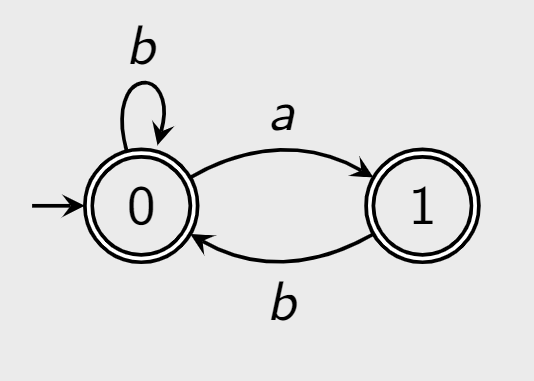
\includegraphics[scale=0.3]{img/cap1/ejemplo7_1.png}
        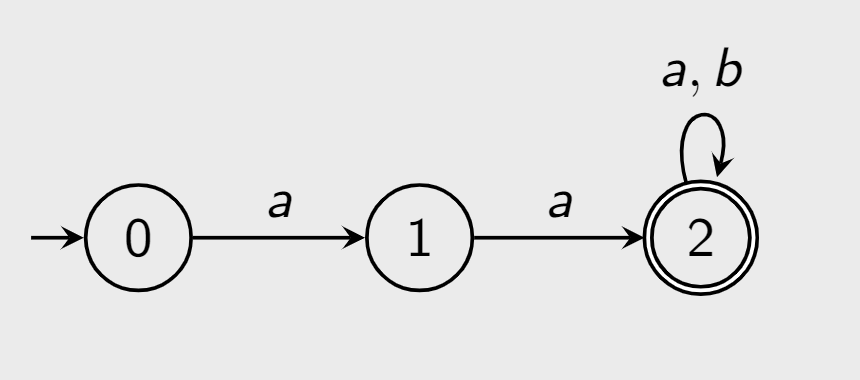
\includegraphics[scale=0.3]{img/cap1/ejemplo7_2.png}
    \end{figure}
}

\paragraph{¿DFA $\not\equiv$ DFAp?} Establezcamos una proposición. Para todo autómata $\ca{A}$ con función parcial de transición, existe un autómata $\ca{A}'$ (con función total de transición) tal que:
\alignformula{
    \ca{L}(\ca{A}) = \ca{L}(\ca{A}')
}
En otras palabras, DFA $\equiv$ DFAp.

\paragraph{Demostración.} Sea $\ca{A} = (Q,\Sigma,\gamma,q_0,F)$ un autómata con función parcial de transición. Sea $q_s$ un \textbf{nuevo estado} tal que $q_s \notin Q$. Contruimos el DFA $\ca{A}' = (Q \cup \{q_s\}, \Sigma, \delta', q_0, F)$ tal que:
$$
    \delta^{\prime}(p, a)= \begin{cases}\gamma(p, a) & \text { si } p \neq q_s \text{ y }(p, a) \in \operatorname{dom}(\gamma) \\ q_s & \text { si no }\end{cases}
$$
para todo $p \in Q \cup \{q_s\}$ y $a \in \Sigma$. Queremos demostrar que $\ca{L}(\ca{A}) = \ca{L}(\ca{A}')$.

\paragraph{Dem. $\ca{L}(\ca{A}) \subseteq \ca{L}(\ca{A}')$.} Sea $w = a_1\ldots a_n \in \ca{L}(\ca{A})$. Entonces, existe una ejecución de aceptación $\rho$ de $\ca{A}$ sobre $w$:
$$
    \rho: p_0 \stackrel{a_1}{\rightarrow} p_1 \stackrel{a_2}{\rightarrow} p_2 \ldots \overset{a_n}{\rightarrow} p_n
$$
donde $p_0 = q_0$, para todo $i \in \{0,\ldots,n-1\}$ está definido $\gamma(p_i,a_{i+1}) = p_{i+1}$ y $p_n \in F$. Como $\delta'(p_i, a_{i+1}) = \gamma(p_i,a_{i+1})$ para todo $i \in \{0,\ldots,n-1\}$ (por la definición de $\delta'$), entonces $\rho$ es también una ejecución de aceptación de $\ca{A}'$ sobre $w$. Por lo tanto, $w \in \ca{L}(\ca{A}')$.

\paragraph{Dem. $\ca{L}(\ca{A}') \subseteq \ca{L}(\ca{A})$.} Sea $w = a_1\ldots a_n \in \ca{L}(\ca{A}')$. Entonces, existe una ejecución de aceptación $\rho$ de $\ca{A}'$ sobre $w$:
$$
    \rho: p_0 \stackrel{a_1}{\rightarrow} p_1 \stackrel{a_2}{\rightarrow} p_2 \ldots \overset{a_n}{\rightarrow} p_n
$$
donde $p_0 = q_0$, para todo $i \in \{0,\ldots,n-1\}$ tenemos $\gamma'(p_i,a_{i+1}) = p_{i+1}$ y $p_n \in F$. Demostraremos que $p_i \neq q_s$ para todo $i \in \{0,\ldots, n\}$. Por \textbf{contradicción}, suponga que existe $i$ tal que $p_i = q_s$. Entonces, tenemos que $p_{i+1} = q_s$. Por \textbf{inducción}, podemos demostrar que $p_j = q_s$ para todo $j \ge i$, y así, podemos concluir que $p_n = q_s$, llevándonos a una contradicción. Como $p_i \neq q_s$ para todo $i \in \{0, \ldots, n\}$, tenemos que:
$$
    \delta^{\prime}\left(p_i, a_{i+1}\right)=\gamma\left(p_i, a_{i+1}\right) \quad \forall i \in\{0,1, \ldots, n-1\}
$$
y entonces $\rho$ es una \textbf{ejecución de aceptación} de $\ca{A}$ sobre $w$. Por lo tanto, concluimos que $w \in \ca{L}(\ca{A})$. \hfill $\blacksquare$

\paragraph{Advertencia.} Desde ahora, se utilizaran autómatas con funciones \textbf{totales} de transición, pero sin pérdida de generalidad, en algunos ejemplos habrán autómatas con funciones \textbf{parciales} de transición por simplicidad.

\subsubsection{Operaciones de conjuntos}
\paragraph{Definiciones.} Dado dos lenguajes $L,L' \subseteq \Sigma^*$ se define:
\alignformula{
    \begin{aligned}
        L^C               & =\left\{w \in \Sigma^* \mid w \notin L\right\}                      \\
        L \cap L^{\prime} & =\left\{w \in \Sigma^* \mid w \in L \wedge w \in L^{\prime}\right\} \\
        L \cup L^{\prime} & =\left\{w \in \Sigma^* \mid w \in L \vee w \in L^{\prime}\right\}
    \end{aligned}
}

Dado dos autómatas $\ca{A}$ y $\ca{A}'$:
\begin{enumerate}
    \item ¿Existe un autómata $\ca{B}$ tal que $\ca{L}(\ca{B}) = \ca{L}(\ca{A})^C$?
    \item ¿Existe un autómata $\ca{B}$ tal que $\ca{L}(\ca{B}) = \ca{L}(\ca{A}) \cap \ca{L}(\ca{A}')$?
    \item ¿Existe un autómata $\ca{B}$ tal que $\ca{L}(\ca{B}) = \ca{L}(\ca{A}) \cup \ca{L}(\ca{A}')$?
\end{enumerate}

\paragraph{Construcción de $\ca{L}(\ca{A})^C$.} Dado un autómata $\ca{A} = (Q, \Sigma, \delta, q_0, F)$, definimos el autómata:
\alignformula{
    \mathcal{A}^C=\left(Q, \Sigma, \delta, q_0, Q \backslash F\right)
}
\teorema{}{}{
    Para todo autómata $\ca{A}$, se tiene que $\ca{L}(\ca{A})^C = \ca{L}(\ca{A}^C)$.
}

\paragraph{Producto de autómatas.} Suponga que:
$$
    \begin{aligned}
        \mathcal{A}          & =\left(Q, \Sigma, \delta, q_0, F\right)                                     \\
        \mathcal{A}^{\prime} & =\left(Q^{\prime}, \Sigma, \delta^{\prime}, q_0^{\prime}, F^{\prime}\right)
    \end{aligned}
$$
y considere una palabra $w \in \Sigma^*$. ¿Cómo ejecutamos ambos autómatas sobre $w$ al \textbf{mismo tiempo}? La idea es ejecutar $\ca{A}$ y $\ca{A}'$ \textbf{en paralelo}. Así, definimos el \textbf{producto} entre $\ca{A}$ y $\ca{A}'$ como el autómata $\ca{A} \times \ca{A}' = (Q^\times, \Sigma, \delta^\times, q_0^\times, F^\times)$ tal que:
\begin{itemize}
    \item $Q^\times = Q \times Q'=\{(q,q')\;|\;q\in Q \wedge q' \in Q'\}$
    \item $\delta^\times((q,q'),a)=(\delta(q,a),\delta'(q',a))$
    \item $q^\times_0=(q_0,q'_0)$
    \item $F^\times=F\times F'$
\end{itemize}

\ejemplo{}{}{
    Todas las palabras sobre $\{a,b\}$ con una cantidad par de $a$-letras tal que no hay dos $a$-letras seguidas.
    \img{img/cap1/ejemplo8.png}{0.4}
}

\teorema{}{}{
    Para todo par de autómatas $\ca{A}$ y $\ca{A}'$ se tiene que
    $$
        \ca{L}(\ca{A} \times \ca{A}') = \ca{L}(\ca{A}) \cap \ca{L}(\ca{A}')
    $$
}

\paragraph{Demostración teorema 2.} Solo se demostrará que $\ca{L}(\ca{A}) \cap \ca{L}(\ca{A}') \subseteq \ca{L}(\ca{A} \times \ca{A}')$, la otra dirección queda propuesta para el lector. \medbreak

Sea $w = a_1 \ldots a_n \in \ca{L}(\ca{A}) \cap \ca{L}(\ca{A}')$. Entonces $w \in \ca{L}(\ca{A})$ y $w \in \ca{L}(\ca{A}')$. Existen ejecuciones de aceptación $\rho$ y $\rho'$ de $\ca{A}$ y $\ca{A}'$ sobre $w$, respectivamente:
$$
    \rho: p_0 \stackrel{a_1}{\rightarrow} p_1 \stackrel{a_2}{\rightarrow} \ldots \stackrel{a_n}{\rightarrow} p_n \quad \rho^{\prime}: p_0^{\prime} \stackrel{a_1}{\rightarrow} p_1^{\prime} \stackrel{a_2}{\rightarrow} \ldots \stackrel{a_n}{\rightarrow} p_n^{\prime}
$$
\begin{itemize}
    \item $p_0 = q_0$ y $p_0' = q_0'$.
    \item $\delta(p_{i-1},a_i) = p_i$ y $\delta'(p_{i-1}',a_i) = p_i$ para todo $i \in \{1,\ldots, n\}$.
    \item $p_n \in F$ y $p_n' \in F'$.
\end{itemize}

Por definición, tenemos que: $\rho^{\times}:\left(p_0, p_0^{\prime}\right) \stackrel{a_1}{\rightarrow}\left(p_1, p_1^{\prime}\right) \stackrel{a_2}{\rightarrow} \ldots \stackrel{a_n}{\rightarrow}\left(p_n, p_n^{\prime}\right)$
\begin{itemize}
    \item $(p_0,p_0') = (q_0,q_0')$.
    \item $\left(p_i, p_i^{\prime}\right)=\left(\delta\left(p_{i-1}, a_i\right), \delta^{\prime}\left(p_{i-1}^{\prime}, a_i\right)\right)=\delta^{\times}\left(\left(p_{i-1}, p_{i-1}^{\prime}\right), a_i\right) \forall i \in\{1, \ldots, n\}$.
    \item $(p_n,p_n') \in F \times F'$.
\end{itemize}

Por lo tanto, $\rho^\times$ es una ejecución de $\ca{A} \times \ca{A}'$ sobre $w$ y $w \in \ca{L}(\ca{A} \times \ca{A}')$. \hfill $\blacksquare$

\paragraph{Unión de autómatas.} Sabemos que
$$
    \mathcal{L}(\mathcal{A}) \cup \mathcal{L}\left(\mathcal{A}^{\prime}\right)=\left(\mathcal{L}(\mathcal{A})^C \cap \mathcal{L}\left(\mathcal{A}^{\prime}\right)^C\right)^C
$$

Para calcular el autómata que acepta el lenguaje $\ca{L}(\ca{A}) \cup \ca{L}(\ca{A}')$:
\begin{enumerate}
    \item Complementamos $\ca{A}$ y $\ca{A}'$.
    \item Intersectamos $\ca{A}^C$ y $(\ca{A}')^C$.
    \item Complementamos $\ca{A}^C \times (\ca{A}')^C$.
\end{enumerate}

\subsection{No-determinismo}

\textit{``Indeterminism is the concept that events (certain events, or events of certain types) are not caused deterministically (cf.  causality) by prior events. It is the opposite of \textbf{determinism} and related to chance. It is highly relevant to the philosophical problem of \textbf{free will}.''} - Wikipedia.

\subsubsection{Definición de un NFA}

\paragraph{Definición.} Un autómata finito \textbf{no-determinista} (NFA) es una estructura:
\alignformula{
    \ca{A} = (Q,\Sigma, \Delta, I, F)
}
\begin{itemize}
    \item $Q$ es un conjunto finito de estados.
    \item $\Sigma$ es el alfabeto del input.
    \item $F \subseteq Q$ es el conjunto de estados finales (o aceptación).
    \item $\Delta \subseteq Q \times \Sigma \times Q$ es la \textbf{relación de transición}.
    \item $I \subseteq Q$ es un \textbf{conjunto de estados iniciales}.
\end{itemize}

\ejemplo{}{}{
    \begin{itemize}
        \item $Q = \{0,1,2\}$, $\Sigma = \{a,b\}$, $I = \{0,1\}$, $F = \{2\}$
        \item $\Delta \subseteq Q \times \Sigma \times Q$ se define como:
              \img{img/cap1/ejemplo9.png}{0.4}
    \end{itemize}
}

\paragraph{Ejecución.} Sea $\ca{A} = (Q,\Sigma,\Delta, I, F)$ un NFA y $w = a_1 a_2 \ldots a_n \in \Sigma^*$ el input. Una \textbf{ejecución} (o \textit{run}) $\rho$ de $\ca{A}$ sobre $w$ es una secuencia:
\alignformula{
    \rho: p_0 \stackrel{a_1}{\rightarrow} p_1 \stackrel{a_2}{\rightarrow} \ldots \stackrel{a_n}{\rightarrow} p_n
}
donde $p_0 \in I$ y para todo $i \in \{0,\ldots,n-1\}$, se tiene que $(p_i, a_{i+1}, p_{i+1}) \in \Delta$. \medbreak

Una ejecución $\rho$ de $\ca{A}$ sobre $w$ es de \textbf{aceptación} si $p_n \in F$.

\paragraph{Aceptación.} Decimos que $\ca{A}$ \textbf{acepta} $w$ si \textbf{existe} una ejecución de $\ca{A}$ sobre $w$ que es de aceptación. Por otro lado, decimos que $\ca{A}$ \textbf{rechaza} si \textbf{todas} las ejecuciones de $\ca{A}$ sobre $w$ NO son de aceptación. Además, el \textbf{lenguaje aceptado} por $\ca{A}$ se define como:
\alignformula{
    \ca{L}(\ca{A}) = \{w \in \Sigma^* \mid \ca{A} \text{ acepta } w\}
}

\paragraph{Interpretación.} Las siguientes interpretaciones pueden ayudar a entender mejor un NFA:
\begin{enumerate}
    \item $\Delta \subseteq Q \times \Sigma \times Q$ es la \textbf{relación de transición}.

          \textit{``$(q,a,p) \in \Delta$ entonces existe una transición desde $q$ a $p$ al leer $a$''.}

    \item $I \subseteq Q$ es un \textbf{conjunto de estados iniciales}.

          \textit{``$p \in I$ entonces $p$ es un posible estado inicial del autómata''}

    \item[$1'$.] $\Delta: Q \times \Sigma \to 2^Q$ es una \textbf{función de transición}.

        \textit{``$q \in \Delta(p,a)$ entonces $q$ es un posible estado que puedo llegar desde $p$ al leer $a$''.}

        Esta interpretación es más común encontrarla en libros sobre teoría de autómatas.
\end{enumerate}

Además, el \textbf{no-determinismo} puede ser visto como:
\begin{enumerate}
    \item Paralelización infinita, es decir, cada ejecución es un \textit{thread} distinto.
    \item ``Guessing and Verifying'' (adivinar y verificar).
\end{enumerate}

El no-determinismo NO debe ser visto como:
\begin{itemize}
    \item Explicitamente como el \textbf{indeterminismo} o ``libre albedrío''. Para un input, un NFA siempre produce el mismo resultado.
    \item Comportamiento \textbf{aleatorio} del autómata.
\end{itemize}

\fig{img/cap1/nodeterminismo.png}{0.275}{Interpretación del no-determinismo}

\subsubsection{Comparación con DFA}

A continuación, veremos que autómata finito determinista (DFA) puede almacenar \textbf{todas} las ejecuciones de un NFA. A este proceso se le conoce como \textbf{determinización}.

\teorema{}{}{
    Para todo autómata finito no-determinista $\ca{A}$, existe un autómata determinista $\ca{A}'$ tal que
    $$
        \ca{L}(\ca{A}) = \ca{L}(\ca{A}')
    $$
    En otras palabras, DFA $\equiv$ NFA.
}

\paragraph{Idea.} Primero, pensemos en la idea de determinización: \textit{``almacenar en el autómata determinista todos los estados actuales de las ejecuciones en curso (sin repetidos)''}.

\ejemplo{}{}{
    \img{img/cap1/ejemplo10.png}{0.325}
}

\paragraph{Formalización.} Para un autómata no-determinista $\ca{A} = (Q,\Sigma,\Delta,I,F)$, definimos el autómata determinista (\textbf{determinización} de $\ca{A}$):
\alignformula{
\ca{A}^{\text{det}} = (2^Q,\Sigma,\delta^{\text{det}},q_0^\text{det},F^\text{det})
}
\begin{itemize}
    \item $2^Q = \{S \mid S\subseteq Q\}$ es el conjunto potencia de $Q$.
    \item $q_0^\text{det} = I$.
    \item $\delta^\text{det}: 2^Q \times \Sigma \to 2^Q$ tal que:
          $$
              \delta^\text{det}(S,a) = \{q \in Q \mid \exists p \in S.\ (p,a,q) \in \Delta\}
          $$
    \item $F^\text{det} = \{S \in 2^Q \mid S \cap F \neq \varnothing\}$, es decir, todos los conjuntos que tengan al menos un estado final.
\end{itemize}

\paragraph{Demostración teorema 3.} La determinización puede verse como un \textbf{subset construction}. Partamos con $\ca{L}(\ca{A}) \subseteq \ca{L}(\ca{A}^\text{det})$. \medbreak

Sea $w = a_1\ldots a_n \in \ca{L}(\ca{A})$. Existe una ejecución $\rho$ de $\ca{A}$ sobre $w$:
$$
    \rho: p_0 \stackrel{a_1}{\rightarrow} p_1 \stackrel{a_2}{\rightarrow} \ldots \stackrel{a_n}{\rightarrow} p_n
$$
donde $p_0 = I$, $(p_i, a_{i+1},p_{i+1}) \in \Delta$ para todo $i \in \{0,\ldots,n-1\}$ y $p_n \in F$. \medbreak

Como $\ca{A}^\text{det}$ es determinista, entonces existe una ejecución $\rho'$ de $\ca{A}^\text{det}$ sobre $w$:
$$
    \rho^{\prime}: S_0 \stackrel{a_1}{\rightarrow} S_1 \stackrel{a_2}{\rightarrow} \ldots \stackrel{a_n}{\rightarrow} S_n
$$
donde $S_0 = I$ y $\delta^\text{det}(S_i, a_{i+1}) = S_{i+1}$ para todo $i \in \{0,\ldots,n-1\}$. Luego, queremos demostrar que $p_i \in S_i$ para todo $i \in \{0,\ldots,n-1\}$. \medbreak

Por \textbf{inducción} sobre $i$, tenemos que:
\begin{itemize}
    \item \textbf{Caso base:} $p_0 \in S_0$ por definición de $\ca{A}^\text{det}$.
    \item \textbf{Inducción:} Suponemos que $p_i \in S_i$ y demostramos para $i+1$. Como sabemos que:
          \begin{itemize}
              \item $\delta^\text{det}(S_i,a_{i+1})=S_{i+1} = \{q \in Q \mid \exists p \in S_i.\ (p,a,q) \in \Delta \}$ y
              \item $(p_i,a_{i+1},p_{i+1}) \in \Delta$
          \end{itemize}
          Entonces $p_{i+1} \in S_{i+1}$, ya que, si estamos en $p_i$ leyendo $a_{i+1}$, la transición nos dice que pasaremos al estado $p_{i+1}$ que pertenece a $S_{i+1}$ por la hipótesis de inducción.
\end{itemize}
Luego, como $p_n \in S_n$, entonces $S_n \cap F \neq \varnothing$ y así $S_n \in F^\text{det}$. Por lo tanto, $w \in \ca{L}(\ca{A}^\text{det})$. \medbreak

Ahora, demostramos la otra dirección: $\ca{L}(\ca{A}^\text{det}) \subseteq \ca{L}(\ca{A})$. \medbreak

Sea $w = a_1\ldots a_n \in \ca{L}(\ca{A}^\text{det})$. Existe una ejecución $\rho$ de $\ca{A}^\text{det}$ sobre $w$:
$$
    \rho: S_0 \stackrel{a_1}{\rightarrow} S_1 \stackrel{a_2}{\rightarrow} \ldots \stackrel{a_n}{\rightarrow} S_n
$$
donde $S_0 = I$, $\delta^\text{det}(S_i, a_{i+1}) = S_{i+1}$ para todo $i \in \{0,\ldots,n-1\}$ y $S_n \in F^\text{det}$, con $S_n \cap F \neq \varnothing$. Buscamos demostrar entonces que para todo $i \leq n$ y para todo $p \in S_i$, existe una ejecución:
$$
    \rho: p_0 \stackrel{a_1}{\rightarrow} p_1 \stackrel{a_2}{\rightarrow} \ldots \stackrel{a_i}{\rightarrow} p_i=p
$$
tal que:
\begin{enumerate}
    \item $p_0 \in I$.
    \item $(p_j, a_{j+1}, p_{j+1}) \in \Delta$ para todo $j \in \{0,\ldots,i-1\}$.
\end{enumerate}
Por \textbf{inducción} sobre $i$, tenemos que:
\begin{itemize}
    \item \textbf{Caso base:} Si $p \in S_0 = I$, entonces la ejecución $\rho: p$ cumple 1. y 2.
    \item \textbf{Inducción:} Supongamos que se cumple para todo $p \in S_i$. Sea $q \in S_{i+1}$. Como $\delta^\text{det}(S_i,a_{i+1})=S_{i+1}=\{q \in Q \mid \exists p \in S_i.\ (p,a,q)\in \Delta\}$ y $q \in S_{i+1}$, entonces existe $p \in S_i$ tal que $(p,a_{i+1},q) \in \Delta$.
\end{itemize}
Por hipótesis de inducción, existe $\rho: p_0 \stackrel{a_1}{\rightarrow} p_1 \stackrel{a_2}{\rightarrow} \ldots \stackrel{a_i}{\rightarrow} p_i=p$ que satisface 1. y 2. \medbreak

Por lo tanto, $\rho^{\prime}: p_0 \stackrel{a_1}{\rightarrow} p_1 \stackrel{a_2}{\rightarrow} \ldots \stackrel{a_i}{\rightarrow} p_i \stackrel{a_{i+1}}{\rightarrow} q$ también satisface 1. y 2. \medbreak

Como lo anterior queda demostrado y como $S_n \cap F \neq \varnothing$, para $p \in S_n \cap F$ existe una ejecución de aceptación de $\ca{A}$ sobre $w$. Por lo tanto, $w \in \ca{L}(\ca{A})$. \hfill $\blacksquare$

\subsection{Expresiones regulares}

\paragraph{Definición.} $R$ es una \textbf{expresión regular} sobre $\Sigma$ si $R$ es igual a:
\begin{enumerate}
    \item $a$, para alguna letra $a \in \Sigma$.
    \item $\epsilon$
    \item $\varnothing$
    \item $(R_1 + R_2)$, donde $R_1$ y $R_2$ son expresiones regulares.
    \item $(R_1 \cdot R_2)$, donde $R_1$ y $R_2$ son expresiones regulares.
    \item $(R_1^*)$, donde $R_1$ es una expresión regular. Esta expresión se conoce como \textbf{clausura de Kleene}.
\end{enumerate}

Denotaremos como ExpReg el conjunto de \textbf{todas las expresiones regulares} sobre $\Sigma$.

\ejemplo{}{}{
    Las siguientes son expresiones regulares sobre $\Sigma=\{a,b\}$:
    \begin{itemize}
        \item $(a+b)$
        \item $((a\cdot b) \cdot c)$
        \item $(a^*)$
        \item $(b \cdot (a^*))$
        \item $((a+b)^*)$
        \item $((a \cdot ((b\cdot a)^*))+\epsilon)$
        \item $((a \cdot ((b\cdot a)^*))+\varnothing)$
    \end{itemize}
}

Para reducir la cantidad de paréntesis, se define el \textbf{orden de precendencia}:
\begin{enumerate}
    \item estrella $(\cdot)^*$
    \item concanetación $\cdot$
    \item unión $+$
\end{enumerate}

\paragraph{Semántica.} Para una expresión regular $R$ cualquiera, se define el lenguaje $\ca{L}(R) \subseteq \Sigma^*$ \textbf{inductivamente} como:
\begin{enumerate}
    \item $\ca{L}(a) = \{a\}$, para toda letra $a \in \Sigma$.
    \item $\ca{L}(\epsilon) = \{\epsilon\}$.
    \item $\ca{L}(\varnothing) = \varnothing$.
    \item $\ca{L}(R_1 + R_2) = \ca{L}(R_1) \cup \ca{L}(R_2)$, donde $R_1$ y $R_2$ son expresiones regulares.
    \item $\ca{L}(R_1 \cdot R_2) = \ca{L}(R_1)\cdot \ca{L}(R_2)$, donde $R_1$ y $R_2$ son expresiones regulares.
    \item $\ca{L}(R_1^*)=\displaystyle\bigcup_{k=0}^\infty \ca{L}(R_1)^k$, donde $R_1$ es una expresión regular.
\end{enumerate}

Para el punto 5. y 6., definimos para dos lenguajes $L_1,L_2 \subseteq \Sigma^*$ el \textbf{producto} de $L_1$ y $L_2$:
\alignformula{
    L_1 \cdot L_2 = \{ w_1 \cdot w_2 \mid w_1 \in L_1 \wedge w_2 \in L_2 \}
}
Además, para un lenguaje $L\subseteq \Sigma^*$ se define la \textbf{potencia} a la $n \ge 0$:
\alignformula{
    L^n = \{ w_1 \cdot w_2 \ldots w_n \mid \forall i\leq n.\ w_i \in L \}
}
La \textbf{potencia} a la $0$ se define como $L^0 = \{\epsilon\}$.

\ejemplo{}{}{
    Se muestran a continuación lenguajes definidos por algunas ExpReg:
    \begin{itemize}
        \item $\ca{L}((a+b)^*) = \{a,b\}^*$
        \item $\ca{L}((a\cdot b)\cdot (b\cdot a)) = \{abba\}$
        \item $\ca{L}(a \cdot (b\cdot a) + b\cdot a + (a\cdot b)\cdot a) = \{aba,ba\}$
    \end{itemize}
}

\paragraph{Definición.} Decimos que $R_1$ es \textbf{equivalente} a $R_2$ si, y sólo si, $\ca{L}(R_1) = \ca{L}(R_2)$. Si $R_1$ es equivalente a $R_2$, escribiremos $R_1 \equiv R_2$.

\paragraph{Lema.} Los operadores de unión $+$ y producto $\cdot$ son \textbf{asociativos}.
\alignformula{
    (R_1 + R_2) + R_3 &\equiv R_1 + (R_2 + R_3)\\
    (R_1 \cdot R_2) \cdot R_3 &\equiv R_1 \cdot (R_2 \cdot R_3)
}

La demostración de este lema queda como ejercicio propuesto al lector.

\ejemplo{}{}{
    Más lenguajes definidos por algunas ExpReg:
    \begin{itemize}
        \item $\ca{L}(a^* \cdot b \cdot a^*) =$ todas las palabras con una sola $b$.
        \item $\ca{L}((a+b)^* \cdot b \cdot (a+b)^* ) =$ todas las palabras con una o más $b's$.
    \end{itemize}
}

\paragraph{Definición.} Usamos las siguientes \textbf{abreviaciones} de expresiones regulares:
\alignformula{
    R^+ &\equiv R \cdot R^* \\
    R^k &\equiv R \cdot \ \overset{k}{\cdots} \ \cdot R \\
    R^? &\equiv R + \epsilon \\
    \Sigma &\equiv a_1 + \ldots + a_n
}
para $R \in \text{ExpReg}$ y $\Sigma = \{a_1,\ldots,a_n\}$.

\ejemplo{}{}{
    Más lenguajes definidos por algunas ExpReg:
    \begin{itemize}
        \item $\ca{L}(\Sigma^* \cdot b \cdot \Sigma^*) =$ todas las palabras con una sola $b$.
        \item $\ca{L}(b^* \cdot (a\cdot b)^5) =$ todas las palabras con $5$ $a$'s.
        \item $\ca{L}(a^* \cdot (b + c)^?)=$ todas las palabras de $a$'s y terminadas en $b$ o $c$.
        \item $\ca{L}((a\cdot b^+)^+)=$ todas las palabras que empiezan con $a$ y donde cada $a$ esta seguida de al menos una $b$.
    \end{itemize}
}

\subsection{Autómatas con transiciones sin lectura}
Hasta ahora, hemos visto lo siguiente:
\fig{img/cap1/mapa1.png}{0.25}{Mapa actual de nuestros modelos de computación}

Podemos demostrar que ExpReg $\subseteq$ NFA, pero para eso necesitamos un nuevo modelo.

\subsubsection[e-NFA]{$\epsilon$-NFA}

Lo nuevo de este autómata:
\begin{enumerate}
    \item tiene transiciones no deterministas y
    \item tiene transiciones leyendo la palabra vacía $\epsilon$:
          $$
              p \overunder{\to}{}{\epsilon} q
          $$
\end{enumerate}

La importancia de un $\epsilon$-NFA es que es un modelo \textbf{muy útil} para construir nuevos autómatas y NO agrega más poder de computación a los NFA.

\paragraph{Definición.} Un autómata finito no-determinista con $\epsilon$-transiciones ($\epsilon$-NFA) es una tupla:
\alignformula{
    \ca{A} = (Q, \Sigma, \Delta, I, F)
}

\begin{itemize}
    \item $Q$ es un conjunto finito de estados.
    \item $\Sigma$ es el alfabeto del input.
    \item $I \subseteq Q$ es un conjunto de estados iniciales.
    \item $F \subseteq Q$ es el conjunto de estados finales (o aceptación).
    \item $\Delta \subseteq Q \times (\Sigma \cup \{\epsilon\}) \times Q$ es la relación de transición.
\end{itemize}

\ejemplo{}{}{
    Algunos ejemplos de $\epsilon$-NFA's:
    \begin{figure}[H]
        \centering
        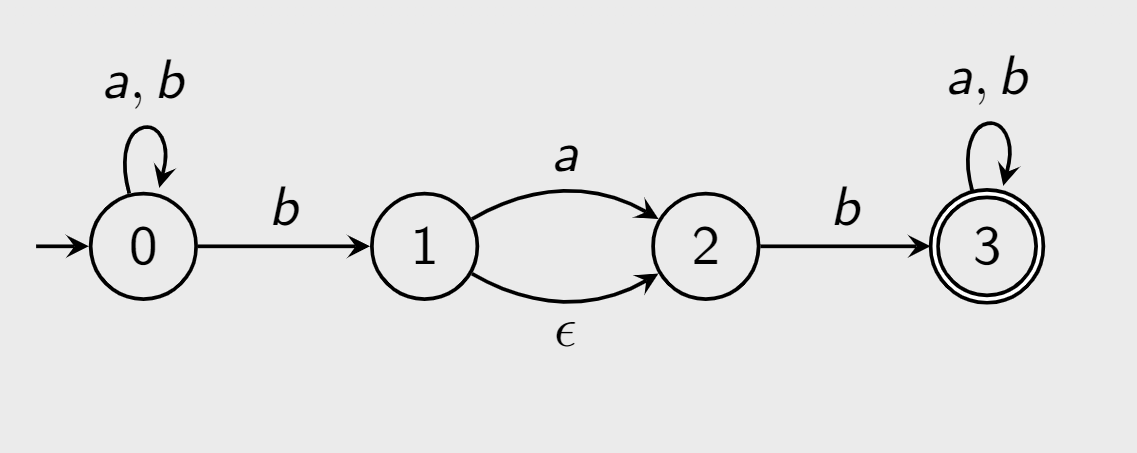
\includegraphics[scale=0.35]{img/cap1/ejemplo15_1.png}
        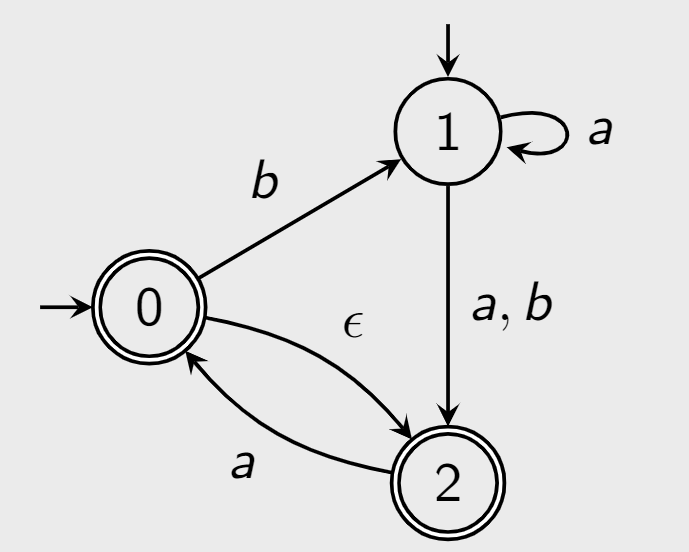
\includegraphics[scale=0.35]{img/cap1/ejemplo15_2.png}
    \end{figure}
}

Para $\epsilon$-NFA veremos una \textbf{forma alternativa} para definir las nociones de ejecución y aceptación.

\paragraph{Ejecución.} Sea $\ca{A} = (Q,\Sigma,\Delta, I, F)$ un $\epsilon$-NFA. Definimos:
\begin{itemize}
    \item Un par $(q,w) \in Q \times \Sigma^*$ es una \textbf{configuración} de $\ca{A}$.
    \item Una configuración $(q,w)$ es \textbf{inicial} si $q \in I$.
    \item Una configuración $(q,w)$ es \textbf{final} si $q \in F$ y $w = \epsilon$.
\end{itemize}

\textit{``Intuitivamente, una configuración $(q, aw)$ representa que $\ca{A}$ se encuentra en el estado $q$ procesando la palabra $aw$ y leyendo $a$''.}
\begin{itemize}
    \item Se define la relación $\vdash_\ca{A}\ \subseteq (Q \times \Sigma^*) \times (Q \times \Sigma^*)$ de \textbf{siguiente-paso} entre configuraciones de $\ca{A}$:
          \alignformula{
              (p, u) \vdash_\ca{A} (q,v)
          }
          si, y sólo si, existe $(p,c,q) \in \Delta$ con $c \in \Sigma \cup \{\epsilon\}$ tal que $u = c \cdot v$.
    \item Se define $\vdash_\ca{A}^*$ como la clausura \textbf{refleja} y \textbf{transitiva} de $\vdash_\ca{A}$:
          \alignformula{
              \text{para toda configuración } (q,w): \qquad &(q,w) \vdash_\ca{A}^* (q,w) \\
              \text{si } (p, u) \vdash_\ca{A} (p',w) \text{ y } (p',w) \vdash_\ca{A}^* (q,v): \qquad &(p, u) \vdash_\ca{A}^* (q,v)
          }
          Decimos que $(p,u) \vdash_\ca{A}^* (q,v)$ si uno puede ir de $(p, u)$ a $(q,v)$ en \textbf{0 o más pasos}.
\end{itemize}

\ejemplo{}{}{
    \img{img/cap1/ejemplo16.png}{0.4}
}

\paragraph{Aceptación.} Sea $\ca{A} = (Q,\Sigma,\Delta, I, F)$ un $\epsilon$-NFA y $w \in \Sigma^*$. Decimos que $\ca{A}$ \textbf{acepta} $w$ si existe una configuración \textbf{inicial} $(q_0, w)$ y una configuración \textbf{final} $(q_f, \epsilon)$ tal que:
\alignformula{
    (q_0, w) \vdash_\ca{A}^* (q_f, \epsilon)
}

Además, el \textbf{lenguaje aceptado} por $\ca{A}$ se define como:
\alignformula{
    \ca{L}(\ca{A}) = \{ w \in \Sigma^* \mid \ca{A} \text{ acepta } w \}
}

\textbf{Nota.} Si $\ca{A}$ no tiene $\epsilon$-transiciones o no-determinismo, esta es una forma \textbf{alternativa} para definir ejecución y aceptación para NFA y DFA.

\subsubsection[NFA versus e-NFA]{NFA versus $\epsilon$-NFA}
Partimos enunciado el siguiente teorema:

\teorema{}{}{
    Para todo autómata finito no-determinista con $\epsilon$-transiciones $\ca{A}$, existe un autómata no-determinista $\ca{A}'$ tal que:
    $$
        \ca{L}(\ca{A}) = \ca{L}(\ca{A}')
    $$
    En otras palabras, NFA $\equiv$ $\epsilon$-NFA.
}

Para demostrar este teorema, mostraremos como construir un autómata no-determinista a partir de un $\epsilon$-NFA removiendo las $\epsilon$-transiciones.

\paragraph{Construcción desde $\epsilon$-NFA a NFA.} Dado un $\epsilon$-NFA $\ca{A} = (Q, \Sigma, \Delta, I, F)$ se define el NFA:
$$
    \ca{A}^{\not\epsilon} =  (Q, \Sigma, \Delta^{\not\epsilon}, I, F^{\not\epsilon})
$$
\begin{multicols}{2}
    \begin{itemize}
        \item para todo $p,q \in Q$, $(p,a,q) \in \Delta^{\not\epsilon}$ si, y sólo si, existe $p' \in Q$ tal que:
              \begin{itemize}
                  \item $(p,\epsilon) \vdash_\ca{A}^* (p', \epsilon)$ y
                  \item $(p', a, q) \in \Delta$.
              \end{itemize}
              \img{img/cap1/demenfa1.png}{0.2}
        \item $F^{\not\epsilon} = \{ p \in Q \mid \exists q \in F.\ (p, \epsilon) \vdash_\ca{A}^* (q, \epsilon)\}$
              \img{img/cap1/demenfa2.png}{0.2}
    \end{itemize}
\end{multicols}
Por definición, si $(p, a, q) \in \Delta$, entonces $(p, a, q) \in \Delta^{\not\epsilon}$ para todo $a \in \Sigma$.

\teorema{}{}{
    Dado un $\epsilon$-NFA $\ca{A} = (Q, \Sigma, \Delta, I, F)$ se tiene que:
    $$
        \ca{L}(\ca{A}) = \ca{L}(\ca{A}^{\not\epsilon})
    $$
}
\paragraph{Demostración teorema 5.} Demostrar el teorema anterior es equivalente a demostrar que para todo $p \in Q$ y $w \in \Sigma^*$:
$$
    \exists q \in F.\ (p,w) \vdash_\ca{A}^* (q, \epsilon) \quad \text{si, y sólo si,} \quad \exists q' \in F^{\not\epsilon}.\ (p, w) \vdash_{\ca{A}^{\not\epsilon}}^* (q', \epsilon)
$$
De aquí, podemos \textbf{concluir} que $\ca{A}$ acepta $w$ si, y sólo si, $\ca{A}^{\not\epsilon}$ acepta $w$. \medbreak

Por \textbf{inducción} sobre el largo de $w$:
\begin{itemize}
    \item \textbf{Caso base:} Para $w = \epsilon$:

          $(\Rightarrow)$ Sea $q \in F$ tal que $(p, \epsilon) \vdash_\ca{A}^* (q, \epsilon)$. Por definición de $F^{\not\epsilon}$, se tiene que $p \in F^{\not\epsilon}$. Por lo tanto, $(p,\epsilon) \vdash_{\ca{A}^{\not\epsilon}}^* (p, \epsilon)$.

          $(\Leftarrow)$ Sea $q' \in F^{\not\epsilon}$ tal que $(p, \epsilon) \vdash_{\ca{A}^{\not\epsilon}}^* (q', \epsilon)$. Como $\ca{A}^{\not\epsilon}$ no tiene $\epsilon$-transiciones, entonces $p = q'$ y $p \in F^{\not\epsilon}$. Por definición de $F^{\not\epsilon}$, existe $q \in F$ tal que $(p, \epsilon) \vdash_\ca{A}^* (q, \epsilon)$.

    \item \textbf{Caso inductivo:} Sea $w = a\cdot u$ y $p \in Q$:

          $(\Leftarrow)$ Sea $q' \in F^{\not\epsilon}$ tal que $(p, au) \vdash_{\ca{A}^{\not\epsilon}}^* (q', \epsilon)$. Por definición de $\vdash_{\ca{A}^{\not\epsilon}}^*$ existen $p' \in Q$ tal que:
          $$
              (p, au) \overset{(1)}{\vdash_{\ca{A}^{\not\epsilon}}} (p', u) \overset{(2)}{\vdash_{\ca{A}^{\not\epsilon}}^*} (q', \epsilon)
          $$
          Por $(1)$ sabemos que $(p,au) \vdash_{\ca{A}}^* (p', u)$. \hfill $(3)$

          Como $|u| < |au|$ y por $(2)$, por \textbf{HI} existe $q \in F$: $(p', u) \vdash_\ca{A}^* (q, \epsilon)$. \hfill $(4)$

          Juntando $(3)$ y $(4)$, tenemos que $(p,au) \vdash_\ca{A}^* (q,\epsilon)$.

          $(\Rightarrow)$ Sea $q \in F$ tal que $(p,au) \vdash_\ca{A}^* (q, \epsilon)$. Por definición de $\vdash_\ca{A}^*$ existen $p',p'' \in Q$ tal que:
          $$
              (p, au) \overset{(1)}{\vdash_\ca{A}^*} (p', au) \overset{(2)}{\vdash_\ca{A}} (p'', u) \overset{(3)}{\vdash_\ca{A}^*} (q, \epsilon)
          $$

          Por $(1)$ tenemos que $(p, \epsilon) \vdash_\ca{A}^* (p', \epsilon)$. \hfill $(4)$

          Por $(2)$ tenemos que $(p', a, p'') \in \Delta.$ \hfill $(5)$

          Por $(4)$ y $(5)$, sabemos que $(p, a, p'') \in \Delta^{\not\epsilon}$ y $(p, a \cdot u) \vdash_{\ca{A}^{\not\epsilon}} (p'', u)$. \hfill $(6)$

          Como $|u| < |au|$ y $(3)$, por \textbf{HI} existe $q' \in F^{\not\epsilon}$: $(p'', u) \vdash_{\ca{A}^{\not\epsilon}}^* (q', \epsilon)$. \hfill $(7)$

          Juntando $(6)$ y $(7)$, tenemos que $(p, au) \vdash_{\ca{A}^{\not\epsilon}}^* (q', \epsilon)$. \hfill $\blacksquare$
\end{itemize}

Con el teorema 5 demostrado, nuestro mapa de modelos se ve así:
\fig{img/cap1/mapa2.png}{0.35}{Mapa actual de nuestros modelos de computación}

En la siguiente sección mostraremos que todos definen el mismo conjunto de lenguajes.

\newpage

\subsection{Teorema de Kleene}

\subsubsection{Desde Expresiones a Autómatas}

Veremos a continuación que toda ExpReg se puede transformar en un autómata.

\paragraph{Construcción inductiva.} Para cada $R \in$ ExpReg, construimos un $\epsilon$-NFA $\ca{A}_R$:
\alignformula{
    \ca{A}_R = (Q, \Sigma, \Delta, \{q_0\}, \{q_f\})
}
tal que $\ca{L}(R) = \ca{L}(\ca{A}_R)$.
\paragraph{Casos bases.} Vemos primero los casos base de la construcción inductiva:
\begin{multicols}{3}
    \begin{enumerate}
        \item si $R = a$,

              para alguna letra $a \in \Sigma$:
              \img{img/cap1/RtoA1.png}{0.3}

        \item si $R = \epsilon$:
              \img{img/cap1/RtoA2.png}{0.3}

        \item si $R = \varnothing$:
              \img{img/cap1/RtoA3.png}{0.3}
    \end{enumerate}
\end{multicols}
\begin{enumerate}
    \item[4.] si $R = (R_1 + R_2)$, donde $R_1$ y $R_2$ son expresiones regulares:
        \img{img/cap1/RtoA4_2.png}{0.2}

        Hacemos la construcción inductiva de $R = (R_1 + R_2)$. Sea $\ca{A}_{R_1}$ y $\ca{A}_{R_2}$ los $\epsilon$-NFA para $R_1$ y $R_2$, respectivamente, tal que:
        \begin{itemize}
            \item $\ca{A}_{R_1} = (Q_1, \Sigma, \Delta_1, \{q_0^1\}, \{q_f^1\})$
            \item $\ca{A}_{R_2} = (Q_2, \Sigma, \Delta_2, \{q_0^2\}, \{q_f^2\})$
        \end{itemize}

        Definimos el $\epsilon$-NFA $\ca{A}_{R_1 +R_2} = (Q, \Sigma, \Delta, \{q_0\}, \{q_f\})$ tal que:
        \begin{itemize}
            \item $Q=Q_1 \uplus Q_2 \uplus\left\{q_0, q_f\right\}$
            \item $\Delta=\Delta_1 \uplus \Delta_2 \uplus\left\{\left(q_0, \epsilon, q_0^1\right),\left(q_0, \epsilon, q_0^2\right),\left(q_f^1, \epsilon, q_f\right),\left(q_f^2, \epsilon, q_f\right)\right\}$
        \end{itemize}

        \textbf{Proposición.} Si $R = (R_1 +R_2)$, entonces $\mathcal{L}\left(R_1+R_2\right)=\mathcal{L}\left(\mathcal{A}_{R_1+R_2}\right)$. \medbreak

        La demostración de esta proposición queda como ejercicio propuesto para el lector.

    \item[5.] si $R = (R_1 \cdot R_2)$, donde $R_1$ y $R_2$ son expresiones regulares:
        \img{img/cap1/RtoA5_2.png}{0.2}

        Hacemos la construcción inductiva de $R = (R_1 \cdot R_2)$. Sea $\ca{A}_{R_1}$ y $\ca{A}_{R_2}$ los $\epsilon$-NFA para $R_1$ y $R_2$, respectivamente, tal que:
        \begin{itemize}
            \item $\ca{A}_{R_1} = (Q_1, \Sigma, \Delta_1, \{q_0^1\}, \{q_f^1\})$
            \item $\ca{A}_{R_2} = (Q_2, \Sigma, \Delta_2, \{q_0^2\}, \{q_f^2\})$
        \end{itemize}

        Definimos el $\epsilon$-NFA $\ca{A}_{R_1 \cdot R_2} = (Q, \Sigma, \Delta, \{q_0^1\}, \{q_f^2\})$ tal que:
        \begin{itemize}
            \item $Q=Q_1 \uplus Q_2$
            \item $\Delta=\Delta_1 \uplus \Delta_2 \uplus\left\{\left(q_f^1, \epsilon, q_0^2\right)\right\}$
        \end{itemize}

        \textbf{Proposición.} Si $R = (R_1 \cdot R_2)$, entonces $\mathcal{L}\left(R_1\cdot R_2\right)=\mathcal{L}\left(\mathcal{A}_{R_1\cdot R_2}\right)$. \medbreak

        La demostración de esta proposición queda como ejercicio propuesto para el lector.

    \item[6.] si $R = (R_1^*)$, donde $R_1$ es una expresión regular:
        \img{img/cap1/RtoA6_2.png}{0.2}

        Hacemos la construcción inductiva de $R = (R_1^*)$. Sea $\ca{A}_{R_1}$ el $\epsilon$-NFA para $R_1$, tal que:
        \begin{itemize}
            \item $\ca{A}_{R_1} = (Q_1, \Sigma, \Delta_1, \{q_0^1\}, \{q_f^1\})$
        \end{itemize}

        Definimos el $\epsilon$-NFA $\ca{A}_{(R_1^*)} = (Q, \Sigma, \Delta, \{q_0\}, \{q_0\})$ tal que:
        \begin{itemize}
            \item $Q=Q_1 \uplus\left\{q_0\right\}$
            \item $\Delta=\Delta_1 \biguplus\left\{\left(q_0, \epsilon, q_0^1\right),\left(q_f^1, \epsilon, q_0\right)\right\}$
        \end{itemize}

        \textbf{Proposición.} Si $R = (R_1^*)$, entonces $\mathcal{L}\left(R_1^*\right)=\mathcal{L}\left(\mathcal{A}_{(R_1^*)}\right)$. \medbreak

        La demostración de esta proposición queda como ejercicio propuesto para el lector.
\end{enumerate}

\teorema{}{}{
    Para todo $R \in$ ExpReg, existe un $\epsilon$-NFA $\ca{A}_R$ tal que:
    $$
        \ca{L}(R) = \ca{L}(\ca{A}_R)
    $$
    En otras palabras, ExpReg $\subseteq$ $\epsilon$-NFA.
}

\subsubsection{Desde Autómatas a Expresiones}

Dado un autómata finito no-determinista (que, sin pérdida de generalidad, tiene un estado inicial):
$$
    \ca{A} = (Q, \Sigma, \Delta, q_0, F)
$$
Para $X \subseteq Q$ y $p,q \in Q$, considerar el conjunto:
$$
    \alpha_{p,q}^X \subseteq \Sigma^*
$$
tal que $w = a_1 \ldots a_n \in \alpha_{p,q}^X$ si, y sólo si, existe una \textbf{ejecución}:
$$
    \rho: p_0 \stackrel{a_1}{\rightarrow} p_1 \stackrel{a_2}{\rightarrow} \ldots \stackrel{a_n}{\rightarrow} p_n
$$
\begin{enumerate}
    \item $\left(p_i, a_{i+1}, p_{i+1}\right) \in \Delta$ para todo $i \in [0,n-1]$,
    \item $p_0 = p$,
    \item $p_n = q$, y
    \item $p_i \in X$ para todo $i \in [1,n-1]$.
\end{enumerate}

\textit{``Intuitivamente, $\alpha_{p,q}^X$ es el conjunto de todas las palabras $w$ tal que existe un \textbf{camino} (i.e. ejecución) desde $p$ a $q$ etiquetado por $w$ y \textbf{todos los estados} en este camino están en $X$, con la posible excepción de $p$ y $q$''.} \medbreak

¿Cómo definimos $\ca{L}(\ca{A})$ en términos de $\alpha_{p,q}^X$? Establecemos el siguiente lema:
$$
    \ca{L}(\ca{A}) = \bigcup_{q \in F} \alpha_{q_0,p}^Q
$$

\paragraph{Estrategia.} Conocida como el algoritmo de McNaughton-Yamada:
\begin{enumerate}
    \item Para cada $\alpha_{p,q}^X$, definir \textbf{inductivamente} una expresión regular $R_{p,q}^X$:
          $$
              \ca{L}(R_{p,q}^X) = \alpha_{p,q}^X
          $$

    \item Para $F = \{p_1, \ldots, p_k\}$ definir la \textbf{expresión regular}:
          $$
              R_\ca{A} = R_{q_0, p_1}^Q+R_{q_0, p_2}^Q+\ldots+R_{q_0, p_k}^Q
          $$

    \item Demostrar que:
          $$
              \ca{L}(\ca{A}) = \ca{L}(R_\ca{A})
          $$
\end{enumerate}

\paragraph{Definición inductiva de $R_{p,q}^X$.} Tenemos que:
\begin{itemize}
    \item \textbf{Caso base:} $X = \varnothing$

          Sea $a_1,\ldots,a_k \in \Sigma$ todas las letras tal que:
          $$
              (p, a_i, q) \in \Delta
          $$
          \begin{itemize}
              \item Si $p \neq q$, entonces:
                    $$
                        R_{p, q}^{\varnothing} \stackrel{\text { def }}{\equiv} \begin{cases}a_1+\cdots+a_k & \text { si } k \geq 1 \\ \varnothing & \text { si } k=0\end{cases}
                    $$
              \item Si $p = q$, entonces:
                    $$
                        R_{p, q}^{\varnothing} \stackrel{\text { def }}{\equiv} \begin{cases}a_1+\cdots+a_k+\epsilon & \text { si } k \geq 1 \\ \epsilon & \text { si } k=0\end{cases}
                    $$
          \end{itemize}

    \item \textbf{Caso general:} $X \neq \varnothing$

          Por \textbf{inducción}, suponemos que para todo $r,s \in Q$ y para todo $Y \subset X$, $R_{r,s}^Y$ es una expresión regular tal que:
          $$
              \ca{L}(R_{r,s}^Y) = \alpha_{r,s}^Y
          $$
          Demostramos la construcción para $R_{p,q}^X$ con $p,q \in Q$. Sea $r \in X$ cualquiera:
          $$
              R_{p, q}^X \stackrel{\text { def }}{\equiv} R_{p, q}^{X-\{r\}}+R_{p, r}^{X-\{r\}} \cdot\left(R_{r, r}^{X-\{r\}}\right)^* \cdot R_{r, q}^{X-\{r\}}
          $$
\end{itemize}
\paragraph{Proposición.} Para todo $X \subseteq Q$ y $p,q \in Q$:
$$
    \mathcal{L}\left(R_{p, q}^X\right)=\alpha_{p, q}^X
$$
\paragraph{Corolario.} $\mathcal{L}(\mathcal{A})=\mathcal{L}\left(R_{\mathcal{A}}\right)$

\ejemplo{Algoritmo MNY}{}{
    Considere el autómata:
    \vspace{-10pt}
    \img{img/cap1/ejemplo17.png}{0.175}
    \vspace{-10pt}
    \begin{table}[H]
        \centering
        \begin{tabular}{c|cc}
            $R^{\varnothing}$ & 1     & 2          \\
            \hline 1          & $a^?$ & $b$        \\
            2                 & $a$   & $\epsilon$
        \end{tabular}
    \end{table}
    \vspace{-20pt}
    \begin{table}[H]
        \centering
        \begin{tabular}{c|cc}
            $R^{\{1\}}$ & $1$                                         & $2$                                          \\
            \hline $1$  & $a^?+a^? \cdot\left(a^?\right)^* \cdot a^?$ & $b+a^? \cdot\left(a^?\right)^* \cdot b$      \\
            $2$         & $a+a \cdot\left(a^?\right)^* \cdot a^?$     & $\epsilon+a \cdot\left(a^?\right)^* \cdot b$
        \end{tabular}
    \end{table}
    \vspace{-20pt}
    $$
        \equiv
    $$
    \vspace{-20pt}
    \begin{table}[H]
        \centering
        \begin{tabular}{c|cc}
            $R^{\{1\}}$ & 1       & 2                  \\
            \hline 1    & $a^*$   & $a^* b$            \\
            2           & $a^{+}$ & $\epsilon+a^{+} b$
        \end{tabular}
    \end{table}

    \begin{table}[H]
        \centering
        \begin{tabular}{c|cc}
            $R^{\{1,2\}}$ & 1 & 2 \\
            \hline 1 & $a^*+a^* b\left(\epsilon+a^{+} b\right)^* a^{+}$ & $a^* b+a^* b\left(\epsilon+a^{+} b\right)^*\left(\epsilon+a^{+} b\right)$ \\
            2 & $a^{+}+\left(\epsilon+a^{+} b\right)\left(\epsilon+a^{+} b\right)^* a^{+}$ & $\left(\epsilon+a^{+} b\right)+\left(\epsilon+a^{+} b\right)\left(\epsilon+a^{+} b\right)^*\left(\epsilon+a^{+} b\right)$
            \end{tabular}
    \end{table}
    \vspace{-20pt}
    $$
        \equiv
    $$
    \vspace{-20pt}
    \begin{table}[H]
        \centering
        \begin{tabular}{c|cc}
            $R^{\{1,2\}}$ & 1 & 2 \\
            \hline 1 & $a^*\left(b a^{+}\right)^*$ & $\left(a^* b\right)\left(a^{+} b\right)^*$ \\
            2 & $\left(a^{+} b\right)^* a^{+}$ & $\left(a^{+} b\right)^*$
            \end{tabular}
    \end{table}
}

\section{Propiedades de lenguajes regulares}

\subsection{Lema de bombeo}

\subsection{Minimización de autómatas}

\subsection{Teorema de Myhill-Nerode}

\subsection{Autómatas en dos direcciones}
\section{Algoritmos para lenguajes regulares}

\subsection{Evaluación de expresiones regulares}

\paragraph{Expresiones regulares en la práctica.} El lenguaje para definir expresiones regulares en la práctica se conoce como \textbf{RegEx} (o RexExp). Las sintaxis más usadas para definir \textbf{RegEx} son:
\begin{enumerate}
    \item POSIX (Portable Operating System Interface for uniX).
    \item Perl (PCRE $=$ Perl Compatible Regular Expressions).
\end{enumerate}

\begin{table}[H]
    \centering
    \begin{tabular}{lcc}
                          & RegEx                                     & Teoría                                                       \\
        \hline
        Carácter          & $\texttt{a}$                              & $\mathrm{a}$                                                 \\
        Escape            & $\backslash+$                             & $-$                                                          \\
        Cualquiera        & $\cdot$                                   & $\Sigma$                                                     \\
        Clase             & {$\texttt{[abc]}$}                        & $(a+b+c)$                                                    \\
        Clase consecutivo & {$\texttt{[a-zA-Z]}$}                     & $(a+\cdots+z+A+\cdots+Z)$                                    \\
        Clase exclusivo   & {$\texttt{[} \texttt{\^{}}\texttt{0-9]}$} & $\left(++_{a \in \Sigma-\{0, \ldots, 9\}} \mathrm{a}\right)$ \\
        Alternación       & $\texttt{cat} \mid \texttt{dog}$          & $\mathrm{cat}+\mathrm{dog}$                                  \\
        0 o 1             & $\texttt{R} ?$                            & $R^?$                                                        \\
        1 o más           & $\texttt{R}+$                             & $R^{+}$                                                      \\
        0 o más           & $\texttt{R} *$                            & $R^*$                                                        \\
        entre $n$ y $m$   & $\texttt{R}\{\texttt{n}, \texttt{m}\}$    & $R^n(R+\epsilon)^{m-n}$                                      \\
        Backreference     & $(\mathrm{R}) \backslash 1$               & $?$                                                          \\
        $\ldots$          & $\cdots$                                  & $\cdots$
    \end{tabular}
\end{table}

\paragraph{¿Cómo evaluamos una expresión regular?} Tenemos el siguiente problema:
\begin{table}[H]
    \centering
    \begin{tabular}{ll}
        $\texttt{PROBLEMA:}$ & Evaluación de expresiones regulares              \\
        $\texttt{INPUT:}$    & una expresión regular $R$                        \\
                             & un documento $w$                                 \\
        $\texttt{OUTPUT:}$   & $\texttt{TRUE}$ si, y sólo si, $w \in \ca{L}(R)$
    \end{tabular}
\end{table}

Donde el tamaño del input está dado por:
\begin{itemize}
    \item $|R|:=$ número de letras y operadores.
    \item $|w|:=$ largo del documento.
\end{itemize}

Buscamos un algoritmo polinomial en $\lvert R \rvert$ y $\lvert w\rvert$. Algo a notar es que $\lvert R\rvert <{}<\lvert w \rvert$:
\begin{itemize}
    \item $|R|$ puede ser del orden \textbf{decenas} operadores ($\sim$ 1 KB).
    \item $|w|$ puede ser del orden de \textbf{miles a millones} de símbolos ($\sim$ 100MB).
\end{itemize}

\paragraph{Análisis de tiempo diferenciado.} Tenemos dos tipos:
\begin{itemize}
    \item \textbf{Combined complexity:} expresión y documento son parte del input.
    \item \textbf{Data complexity:} solo documento es parte del input (tamaño de expresión es considerada una constante).
\end{itemize}

Buscamos algoritmos que sean \textbf{lineales en data complexity} y ojalá \textbf{polinomiales en combined complexity}. \medbreak

Volviendo a nuestro problema:
\begin{table}[H]
    \centering
    \begin{tabular}{ll}
        $\texttt{PROBLEMA:}$ & Evaluación de expresiones regulares              \\
        $\texttt{INPUT:}$    & una expresión regular $R$                        \\
                             & un documento $w$                                 \\
        $\texttt{OUTPUT:}$   & $\texttt{TRUE}$ si, y sólo si, $w \in \ca{L}(R)$
    \end{tabular}
\end{table}

Los pasos que podemos seguir para resolverlo son:
\begin{enumerate}
    \item Convertimos $R$ a un $\epsilon$-NFA $\ca{A}_R$.
    \item Verificamos si $w \in \ca{L}(\ca{A}_R)$.
\end{enumerate}
Ahora, el tamaño del input es:
\begin{itemize}
    \item $|w|:=$ largo del documento.
    \item $|\ca{A}|:= |Q| + |\Delta|$.
\end{itemize}

Hay varias soluciones para resolver nuestro problema, que iremos enumerado a continuación.

\paragraph{Solución 1: Backtracking.} Esta solución es la que usa la mayoría de los motores de RegEx en la práctica. Se puede hacer una prueba en \url{https://regexr.com/}.

\paragraph{Solución 2: DFA.} Para un DFA $\ca{A} = (Q,\Sigma,\delta, q_0, F)$ y una palabra $w = a_1 \ldots a_n$.
\vspace{-8pt}
\begin{algorithm}[hbt!]
    % \caption*{An algorithm with caption}\label{alg:two}
    \setstretch{1.25}
    \DontPrintSemicolon
    \SetKwFunction{FevalDFA}{eval-DFA}
    \SetKwProg{Fn}{Function}{:}{}
    \SetKw{Check}{check}
    \Fn{\FevalDFA{$\ca{A}$, $w$}}{
        $q := q_0$

        \For{$i=1$ \KwTo $n$}{
            $q := \delta(q,a_i)$
        }

        \Return{\Check $(q \in F)$}
    }
\end{algorithm}
\vspace{-8pt}
\paragraph{Solución 3: NFA determinización.} Para un NFA $\ca{A} = (Q,\Sigma,\Delta, I, F)$ y una palabra $w = a_1 \ldots a_n$.
\vspace{-8pt}
\begin{algorithm}[hbt!]
    % \caption*{An algorithm with caption}\label{alg:two}
    \setstretch{1.25}
    \DontPrintSemicolon
    \SetKwFunction{FevalNFA}{eval-NFA}
    \SetKwFunction{FevalDFA}{eval-DFA}
    \SetKwProg{Fn}{Function}{:}{}
    \Fn{\FevalNFA{$\ca{A}$, $w$}}{
    $\ca{A}^{\text{det}} := \texttt{NFAtoDFA}(\ca{A})$

    \Return{\FevalDFA{$\ca{A}^{\text{det}},w$}}
    }
\end{algorithm}

¿Es necesario construir la determinización completa? La respuesta es que no. Recordemos que es la determinización. Para un autómata no-determinista $\ca{A} = (Q,\Sigma,\Delta,I,F)$, definimos el autómata determinista (\textbf{determinización} de $\ca{A}$):
\alignformula{
\ca{A}^{\text{det}} = (2^Q,\Sigma,\delta^{\text{det}},q_0^\text{det},F^\text{det})
}
\begin{itemize}
    \item $2^Q = \{S \mid S\subseteq Q\}$ es el conjunto potencia de $Q$.
    \item $q_0^\text{det} = I$.
    \item $\delta^\text{det}: 2^Q \times \Sigma \to 2^Q$ tal que:
          $$
              \delta^\text{det}(S,a) = \{q \in Q \mid \exists p \in S.\ (p,a,q) \in \Delta\}
          $$
    \item $F^\text{det} = \{S \in 2^Q \mid S \cap F \neq \varnothing\}$, es decir, todos los conjuntos que tengan al menos un estado final.
\end{itemize}

\paragraph{Solución 4: NFA \textit{on-the-fly}.} Fijémonos en la función de transición $\delta^\text{det}: 2^Q \times \Sigma \to 2^Q$ tal que:
$$
    \delta^\text{det}(S,a) = \{q \in Q \mid \exists p \in S.\ (p,a,q) \in \Delta\}
$$

La estrategia \textit{on-the-fly} corresponde a:
\begin{enumerate}
    \item Mantenemos un conjunto $S$ de estados actuales.
    \item Por cada nueva letra $a$, calculamos el conjunto $\delta^{\text{det}}(S,a)$.
\end{enumerate}
\fig{img/cap3/nfaonthefly.png}{0.2}{Ejemplo de NFa \textit{on-the-fly}}

Definimos el algoritmo para un NFA $\ca{A}=(Q,\Sigma,\Delta,I,F)$ y una palabra $w = a_1 \ldots a_n$ como:
\vspace{-8pt}
\begin{algorithm}[hbt!]
    % \caption*{An algorithm with caption}\label{alg:two}
    \setstretch{1.25}
    \DontPrintSemicolon
    \SetKwFunction{FevalNFAonthefly}{eval-NFAonthefly}
    \SetKwProg{Fn}{Function}{:}{}
    \SetKw{Check}{check}
    \Fn{\FevalNFAonthefly{$\ca{A}$, $w$}}{
        $S := I$

        \For{$i = 1$ \KwTo $n$}{
            $S_\text{old} := S$

            $S := \varnothing$

            \ForEach{$p \in S_\text{old}$}{
                $S := S \cup \{q \mid (p, a_i,q) \in \Delta\}$
            }
        }

        \Return{\Check $(S \cap F \neq \varnothing)$}
    }
\end{algorithm}

\paragraph{Resumen y complejidades.} Para un autómata $\ca{A}$ y una palabra $w = a_1 \ldots a_n$ tenemos que:

\begin{table}[H]
    \centering
    \begin{tabular}{lc}
                                           & Tiempo                                        \\
        \hline
        Backtracking                       & $\mathcal{O}\left(|\mathcal{A}|^{|w|}\right)$ \\
        DFA                                & $\mathcal{O}(|\mathcal{A}|+|w|)$              \\
        NFA                                & $\mathcal{O}\left(2^{|Q|}+|w|\right)$         \\
        $\epsilon$-NFA \textit{on-the-fly} & $\mathcal{O}(|\mathcal{A}| \cdot|w|)$
    \end{tabular}
\end{table}


\subsection{Transductores}
\fig{img/cap3/transductor.png}{0.2}{Representación de un transductor}

\paragraph{Definición.} Un transductor (en inglés, \textit{transducer}) es una tupla:
\alignformula{
    \ca{T} = (Q,\Sigma,\Omega,\Delta,I,F)
}
\begin{itemize}
    \item $Q$ es un conjunto finito de estados.
    \item $\Sigma$ es el alfabeto del input.
    \item $\Omega$ es el alfabeto del \textbf{output}.
    \item $\Delta \subseteq Q \times(\Sigma \cup\{\epsilon\}) \times(\Omega \cup\{\epsilon\}) \times Q$ es la \textbf{relación de transición}.
    \item $I \subseteq Q$ es un conjunto de estados iniciales.
    \item $F \subseteq Q$ es el conjunto de estados finales.
\end{itemize}

\ejemplo{}{}{
    Algunos transductores:
    \begin{figure}[H]
        \centering
        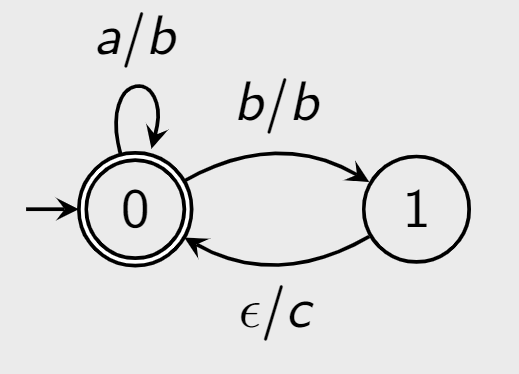
\includegraphics[scale=0.35]{img/cap3/ejemplo1_1.png}
        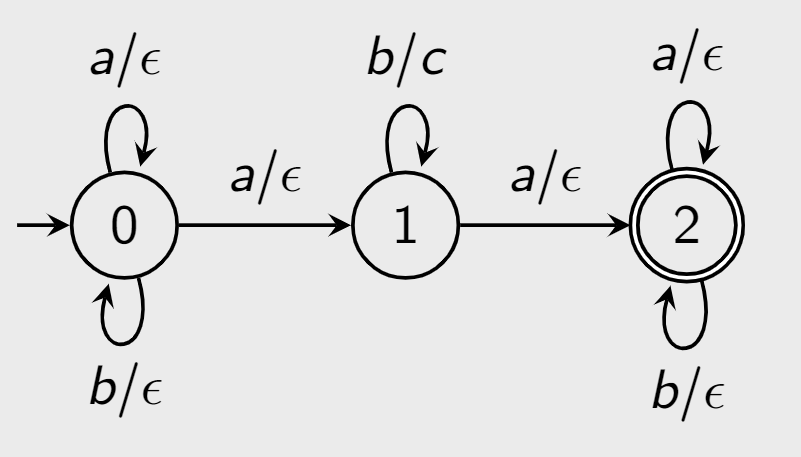
\includegraphics[scale=0.35]{img/cap3/ejemplo1_2.png}
    \end{figure}
}

\paragraph{Configuración.} Sea $\ca{T}$ un transductor. Definimos:
\begin{itemize}
    \item Un par $(q, u, v) \in Q \times \Sigma^* \times \Omega^*$ es una \textbf{configuración} de $\ca{T}$.
    \item Una configuración $(q,u,\epsilon)$ es \textbf{inicial} si $q \in F$.
    \item Una configuración $(q,\epsilon,v)$ es \textbf{final} si $q \in F$.
\end{itemize}

\textit{``Intuitivamente, una configuración $(q, au, vb)$ representa que $\ca{T}$ se encuentra en el estado $q$ procesando la palabra $au$ y leyendo $a$, y hasta ahora grabó la palabra $vb$ y el último símbolo impreso es $b$''.}

\paragraph{Ejecución.} Se define la relación $\vdash_\ca{T}\; \subseteq\left(Q \times \Sigma^* \times \Omega^*\right) \times\left(Q \times \Sigma^* \times \Omega^*\right)$ de \textbf{siguiente-paso} entre configuraciones de $\ca{T}$:
\alignformula{
    \left(p, u_1, v_1\right) \vdash_{\mathcal{T}}\left(q, u_2, v_2\right)
}
si, y sólo si, existe $(p,a,b,q) \in \Delta$ tal que $u_1 = a \cdot u_2$ y $v_2 = v_1 \cdot b$. \medbreak

Se define $\vdash_\ca{T}^*$ como la clausura \textbf{refleja} y \textbf{transitiva} de $\vdash_\ca{T}$:
\alignformula{
    \text{para toda configuración } (q,u,v): \quad &(q, u, v) \vdash_{\mathcal{T}}^*(q, u, v) \\
    \text{si } \left(q_1, u_1, v_1\right) \vdash_{\mathcal{T}}^*\left(q_2, u_2, v_2\right) \text{ y } \left(q_2, u_2, v_2\right) \vdash_{\mathcal{T}}\left(q_3, u_3, v_3\right): \quad &\left(q_1, u_1, v_1\right) \vdash_{\mathcal{T}}^*\left(q_3, u_3, v_3\right)
}
\ejemplo{}{}{
    \vspace{-10pt}
    \img{img/cap3/ejemplo2.png}{0.3}
}

\paragraph{Función definida por un transductor.} Dado un transductor $\ca{T}$, decimos que:
\begin{itemize}
    \item $\ca{T}$ \textbf{entrega} $v$ con \textbf{input} $u$ si existe una configuración inicial $(q_0, u, \epsilon)$ y una configuración final $(q_f, \epsilon, v)$ tal que:
          \alignformula{
              \left(q_0, u, \epsilon\right) \stackrel{\vdash_{\mathcal{T}}^*}{ }\left(q_f, \epsilon, v\right)
          }
    \item Se define la función $\llbracket \mathcal{T} \rrbracket: \Sigma^* \rightarrow 2^{\Omega^*}$:
          \alignformula{
              \llbracket \mathcal{T} \rrbracket(u)=\left\{v \in \Omega^* \mid \mathcal{T} \text { entrega } v \text { con input } u\right\}
          }
    \item Se dice que $f: \Sigma^* \rightarrow 2^{\Omega^*}$ es una \textbf{función racional} si existe un transductor $\ca{T}$ tal que $f=\llbracket \mathcal{T} \rrbracket$.
    \item Un transductor define una función de palabras a conjuntos de palabras.
\end{itemize}

\paragraph{Dos interpretaciones para un transductor.} Podemos ver a $\llbracket \mathcal{T} \rrbracket$ de dos formas:
\begin{enumerate}
    \item $\ca{T}$ define la \textbf{función} $\llbracket \mathcal{T} \rrbracket: \Sigma^* \rightarrow 2^{\Omega^*}$:
          $$
              \llbracket \mathcal{T} \rrbracket(u)=\left\{v \in \Omega^* \mid \mathcal{T} \text { entrega } v \text { con input } u\right\}
          $$
    \item $\ca{T}$ define la \textbf{relación} $\left[\mathcal{T} \rrbracket \subseteq \Sigma^* \times \Omega^*\right.$:
          $$
              (u, v) \in \llbracket \mathcal{T} \rrbracket \quad \text { si, y solo si, } \quad \mathcal{T} \text { entrega } v \text { con input } u
          $$
\end{enumerate}

Desde ahora, hablaremos de función o relación \textbf{indistintamente} y hablaremos de las \textbf{relaciones racionales} (definidas por un transductor).

\paragraph{Lenguaje de input y ouput.} Para una relación $R \subseteq \Sigma^* \times \Omega^*$ se define:
\begin{itemize}
    \item $\pi_1(R)=\left\{u \in \Sigma^* \mid \exists v \in \Omega^* .\ (u, v) \in R\right\}$.
    \item $\pi_2(R)=\left\{v \in \Omega^* \mid \exists u \in \Sigma^* .\ (u, v) \in R\right\}$.
\end{itemize}

\teorema{}{}{
    Si $\ca{T}$ es un transductor, entonces $\pi_1(\llbracket \mathcal{T} \rrbracket)$ y $\pi_2(\llbracket \mathcal{T} \rrbracket)$ son lenguajes regulares sobre $\Sigma$ y $\Omega$, respectivamente.
}

\paragraph{Idea demostración teorema 12.} Para $\ca{T} = (Q,\Sigma,\Omega,\Delta,I,F)$, defina $\ca{A}_1 = (Q, \Sigma, \Delta_1, I, F)$ tal que
$$
    (p, a, q) \in \Delta_1 \quad \text { si, y solo si, } \quad \exists b \in \Omega \cup\{\epsilon\} .\ (p, a, b, q) \in \Delta
$$
y demuestre que $\ca{L}(\ca{A}_1) = \pi_1(\llbracket \mathcal{T} \rrbracket)$.

\teorema{}{}{
    Sea $\ca{T}_1$ y $\ca{T}_2$ dos transductores con $\Sigma$ y $\Omega$ alfabetos de input y output. Las siguientes son \textbf{relaciones racionales}:
    \begin{enumerate}
        \item $$
                  \llbracket \mathcal{T}_1 \rrbracket \cup \llbracket \mathcal{T}_2 \rrbracket=\left\{(u, v) \in \Sigma^* \times \Omega^* \mid(u, v) \in \llbracket \mathcal{T}_1 \rrbracket \vee(u, v) \in \llbracket \mathcal{T}_2 \rrbracket\right\}
              $$
        \item $\llbracket \mathcal{T}_1 \rrbracket \cdot \llbracket \mathcal{T}_2 \rrbracket=\left\{\left(u_1 u_2, v_1 v_2\right) \in \Sigma^* \times \Omega^* \mid\left(u_1, v_1\right) \in \llbracket \mathcal{T}_1 \rrbracket \wedge\left(u_2, v_2\right) \in \llbracket \mathcal{T}_2 \rrbracket\right\}$
        \item $\llbracket \mathcal{T}_1 \rrbracket^*=\bigcup_{k=0}^{\infty} \llbracket \mathcal{T}_1 \rrbracket^k$
    \end{enumerate}
}

La demostración de este teorema queda como ejercicio propuesto al lector.

\teorema{}{}{
    Existen transductores $\ca{T}_1$ y $\ca{T}_2$ sobre $\Sigma$ y $\Omega$ tal que:
    $$
        \llbracket \mathcal{T}_1 \rrbracket \cap \llbracket \mathcal{T}_2 \rrbracket=\left\{(u, v) \in \Sigma^* \times \Omega^* \mid(u, v) \in \llbracket \mathcal{T}_1 \rrbracket \wedge(u, v) \in \llbracket \mathcal{T}_2 \rrbracket\right\}
    $$
    NO es una relación racional.
}
\paragraph{Demostración teorema 14.} Considere los siguientes transductores:
\img{img/cap3/teo14.png}{0.2}
Vemos que $\llbracket \mathcal{T}_1 \rrbracket \cap \llbracket \mathcal{T}_2 \rrbracket=\left\{\left(a^n, b^n c^n\right) \mid n \geq 0\right\}$, pero el lenguaje que define el ouput no es regular, y por lo tanto $\llbracket \mathcal{T}_1 \rrbracket \cap \llbracket \mathcal{T}_2 \rrbracket$ no es racional. \hfill $\blacksquare$

\paragraph{Definición.} Decimos que un transductor $\ca{T}$ define una \textbf{función parcial} si:
\alignformula{
    \text { para todo } u \in \Sigma^* \text { se tiene que }|\llbracket \mathcal{T} \rrbracket(u)| \leq 1 \text {. }
}

\paragraph{Definición.} Decimos que $\ca{T}=(Q,\Sigma,\Omega,\Delta,I,F)$ es \textbf{determinista} si cumple que:
\begin{enumerate}
    \item $\ca{T}$ define una función $\llbracket \mathcal{T} \rrbracket: \Sigma^* \rightarrow \Omega^*$.
    \item para todo $(p,a_1,b_1,q_1)\in\Delta$ y $(p,a_2,b_2,q_2)\in \Delta$, si $a_1=a_2$, entonces
          $$
              b_1=b_2 \quad\text{ y }\quad q_1=q_2
          $$
          Es decir, si tenemos dos transiciones desde un estado $p$ a otros dos estados $q_1$ y $q_2$, y ambas transiciones leen lo mismo: $a_1=a_2$, entonces lo que imprime el transductor y los estados deben ser iguales: $b_1=b_2$ y $q_1=q_2$. Básicamente, buscamos que sean la misma transición.
    \item si $(p,\epsilon,b,q) \in \Delta$, entonces para todo $(p,a',b',q')\in\Delta$, se tiene que
          $$
              (a',b',c')=(\epsilon,b,q)
          $$
          Es decir, si tenemos una $\epsilon$-transición, entonces es la única transición que sale desde $p$.
\end{enumerate}
\ejemplo{}{}{
    \img{img/cap3/ejemplo3.png}{0.35}
}

\subsection{Análisis léxico}

PENDIENTE.

\subsection{Algoritmo de Knuth-Morris-Prat}

\paragraph{Pattern matching.} Veamos el siguiente problema. Dado un \textbf{patrón} $w = w_1 \ldots w_m$ y un documento $d = d_1 \ldots d_n$, encontrar todas las posiciones donde aparece $w$ en $d$, o sea, enumerar:
$$
    \left\{(i, j) \mid w=d_i d_{i+1} \ldots d_j\right\}
$$

Podríamos implementar la siguiente solución ingenua (y poco eficiente):
\vspace{-8pt}
\begin{algorithm}[hbt!]
    % \caption*{An algorithm with caption}\label{alg:two}
    \setstretch{1.25}
    \DontPrintSemicolon
    \SetKw{Output}{output}
    \For{$i=0$ \KwTo $n-m$}{
        $j := 1$

        \While{$j \leq m \wedge w_j = d_{i+j}$}{
            $j := j + 1$
        }

        \If{$j > m$}{
            \Output $(i+1, i+m-1)$
        }
    }
\end{algorithm}
\vspace{-8pt}
\subsubsection{Autómata de un patrón}

\paragraph{Definición.} Dado una palabra $w = w_1 \ldots w_m$, sea el NFA $\ca{A}_w = (Q,\Sigma,\Delta,I, F)$ tal que:
\begin{itemize}
    \item $Q = \{0,1,\ldots,m\}$
    \item $\Delta=\{(0, a, 0) \mid a \in \Sigma\} \cup\left\{\left(i, w_{i+1}, i+1\right) \mid i<m\right\}$
    \item $I = \{0\}$ y $F = \{m\}$.
\end{itemize}
\ejemplo{Palabra $w =$ nano}{}{
    \vspace{-8pt}
    \img{img/cap3/ejemplo4.png}{0.325}
}

Podemos usar $\ca{A}_w$ para encontrar todas las apariciones de $w$ en $w$ haciendo su \textbf{determinización}. \medbreak

\paragraph{Definción.} Sea $\mathcal{A}_w^{\operatorname{det}}=\left(Q^{\operatorname{det}}, \Sigma, \delta^{\operatorname{det}},\{0\}, F^{\operatorname{det}}\right)$ la determinización de $\ca{A}_w$ tal que $Q^\text{det}$ contiene \textbf{solo los estados alcanzables} desde $\{0\}$.

\ejemplo{Palabra $w =$ nano y $d =$ un nano no nana}{}{\
    \vspace{-8pt}
    \img{img/cap3/ejemplo5.png}{0.325}
    $$
        \begin{array}{ccccccccccccccccccc}
            q_0 & q_0 & q_1 & q_0 & q_1 & q_2 & q_3 \checkmark & q_4 & q_0 & q_1 & q_0 & q_0 & q_1 & q_2 & q_3 & q_2 \\
            u   & n   &     & n   & a   & n   & o              &     & n   & o   &     & n   & a   & n   & a         \\
            1   & 2   & 3   & 4   & 5   & 6   & 7              & 8   & 9   & 10  & 11  & 12  & 13  & 14  & 15
        \end{array}
    $$
}

\teorema{}{}{
    Para todo $S \in Q^\text{det}$ y $i \in \{0,1,\ldots,m\}$ se cumple que
    $$
        i \in S \quad \text { si, y solo si, } \quad w_1 \ldots w_i \text { es un sufijo de } w_1 \ldots w_{\max (S)} \text {. }
    $$
}

\paragraph{Corolarios.} Tenemos que:
\begin{itemize}
    \item Para todo $S_1,S_2 \in Q^\text{det}$, si $\max(S_1) = \max(S_2)$, entonces $S_1 = S_2$.
    \item $\ca{A}_w^\text{det}$ tiene $|w| + 1$ estados y a lo más $\ca{O}(|w|^2)$ transiciones.
\end{itemize}

Por lo tanto, encontrar todos los substrings de $w$ en $d$ toma tiempo $\ca{O}(|d| + |w|^2)$.

\paragraph{Demostración teorema 15.} Sea $S \in Q^\text{det}$ un conjunto de estados cualquiera alcanzable desde $\{0\}$. Entonces, existe una palabra $u = a_1 \ldots a_k$ tal que $\hat{\delta}^{\operatorname{det}}(\{0\}, u)=S$. Por la demostración de que $\mathcal{L}\left(\mathcal{A}^{\mathrm{det}}\right)=\mathcal{L}(\mathcal{A})$ para todo NFA $\ca{A}$, sabemos que $j \in S$ si, y sólo si, existe una ejecución $\ca{A}_w$ sobre $u$:
$$
    0=q_0 \stackrel{a_1}{\rightarrow} q_1 \stackrel{a_2}{\rightarrow} \ldots \stackrel{a_k}{\rightarrow} q_k=j
$$
Por la definición de $\ca{A}_w$ esta ejecución es de la forma:
$$
    0 \stackrel{a_1}{\rightarrow} 0 \stackrel{a_2}{\rightarrow} \ldots \stackrel{a_{k-j}}{\rightarrow} 0 \underbrace{\stackrel{a_{k-j+1}}{\rightarrow} 1 \stackrel{a_{k-j+2}}{\rightarrow} 2 \ldots \stackrel{a_k}{\rightarrow}}_{w_1 \ldots w_j} j
$$
Por lo tanto, $w_1 w_2 \ldots w_j$ es sufijo de $a_1 \ldots a_k$. Usaremos este último hecho para demostrar \textbf{ambas} direcciones del teorema, que formalizamos a continuación. \medbreak

\textit{Propiedad.} Para toda $u = a_1\ldots a_k$ tal que $\hat{\delta}^{\operatorname{det}}(\{0\}, u)=S$, y para todo $j \leq m$:
$$
    j \in S \quad \text { si, y solo si, } \quad w_1 \ldots w_j \text { es sufijo de } a_1 \ldots a_k
$$

\textit{Demostración $(\Rightarrow)$.} Como $S$ es alcanzable desde $\{0\}$, entonces existe $u = a_1 \ldots a_k$ tal que $\hat{\delta}^{\operatorname{det}}(\{0\}, u)=S$. Como $\max(S) \in S$, entonces $W_1 \ldots W_{\max }(S)$ es sufijo de $a_1 \ldots a_k$. \medbreak

Suponga que $i \in S$. Entonces $w_1 \ldots w_i$ es sufijo de $a_1 \ldots a_k$. Como $i \leq \max(S)$, entonces:
$$
    a_1 a_2 \ldots a_{k-\max(S)} \overbrace{a_{k-\max(S)+1} \ldots a_{k-i} \underbrace{a_{k-i+1}\ldots a_k}_{w_1\ldots w_i}}^{w_1\ldots w_{\max(S)}}
$$
Por lo tanto, $w_1 \ldots w_i$ es sufijo de $w_1 \ldots w_{\max(S)}$. \medbreak

\textit{Demostración $(\Leftarrow)$.} Como $S$ es alcanzable desde $\{0\}$, entonces existe $u = a_1 \ldots a_k$ tal que $\hat{\delta}^{\mathrm{det}}(\{0\}, u)=S$. Como $\max(S) \in S$, entonces $w_1 \ldots w_{\max(S)}$ es sufijo de $a_1 \ldots a_k$. \medbreak

Suponga que $w_1 \ldots w_i$ es sufijo de $w_1 \ldots w_{\max(S)}$. Como $w_1 \ldots w_i$ es sufijo de $w_1 \ldots w_{\max(S)}$ y $w_1 \ldots w_{\max(S)}$ es sufijo de $u$, entonces $w_1 \ldots w_i$ es sufijo de $u = a_1 \ldots a_k$. \medbreak

Por la ``propiedad'', concluimos que $i \in S$. \hfill $\blacksquare$

\subsubsection[Autómata finito con k-lookahead]{Autómata finito con $k$-lookahead}

\paragraph{Definición}. Se definen los siguientes conjuntos de palabras sobre un alfabeto finito $\Sigma$:
\begin{itemize}
    \item $\Sigma_{\bullet}=\Sigma^* \times \Sigma^*$
    \item $\Sigma_{\bullet}^k=\left\{(u, v) \in \Sigma_{\bullet}\mid |uv| = k\right\}$
\end{itemize}

\paragraph{Notación.} En vez de $(u,v) \in \Sigma_\bullet$, escribiremos $u.v \in \Sigma_\bullet$.

\ejemplo{}{}{
    Si $\Sigma = \{a,b\}$, entonces:
    \begin{itemize}
        \item $ab.ba \in \Sigma_\bullet$ y $.aba \in \Sigma_\bullet$
        \item $ab.ba \in \Sigma_\bullet^4$ y $.aba \in \Sigma_\bullet^3$
    \end{itemize}
}

\paragraph{Definición.} Un autómata finito determinista con $k$-lookahead es una tupla:
\alignformula{
    \ca{A} = (Q, \Sigma, \delta, q_0, F)
}
\begin{itemize}
    \item $Q$ es un conjunto finito de estados.
    \item $\Sigma$ es el alfabeto del input.
    \item $q_0$ es el estado inicial.
    \item $F \subseteq Q$ es el conjunto de estados iniciales.
    \item $\delta: Q \times(\Sigma \cup\{\mathbb{\$}\})_{\bullet}^k \rightarrow Q$ es una función parcial, tal que:
          $$
              \text { para todo } p \in Q \text { y } w \in(\Sigma \cup\{\$\})^k:\quad  |\{u . v \mid \delta(p, u \cdot v)=q \text { y } u v=w\}| \leq 1
          $$
\end{itemize}
\ejemplo{}{}{
    \begin{figure}[H]
        \centering
        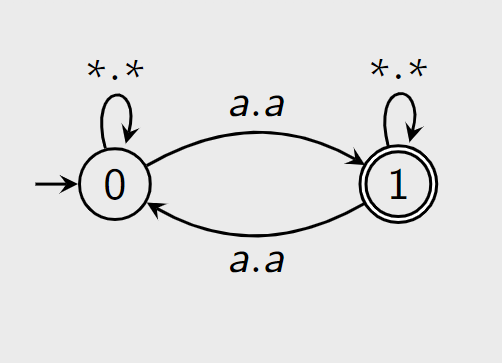
\includegraphics[scale=0.4]{img/cap3/ejemplo6_1.png}
        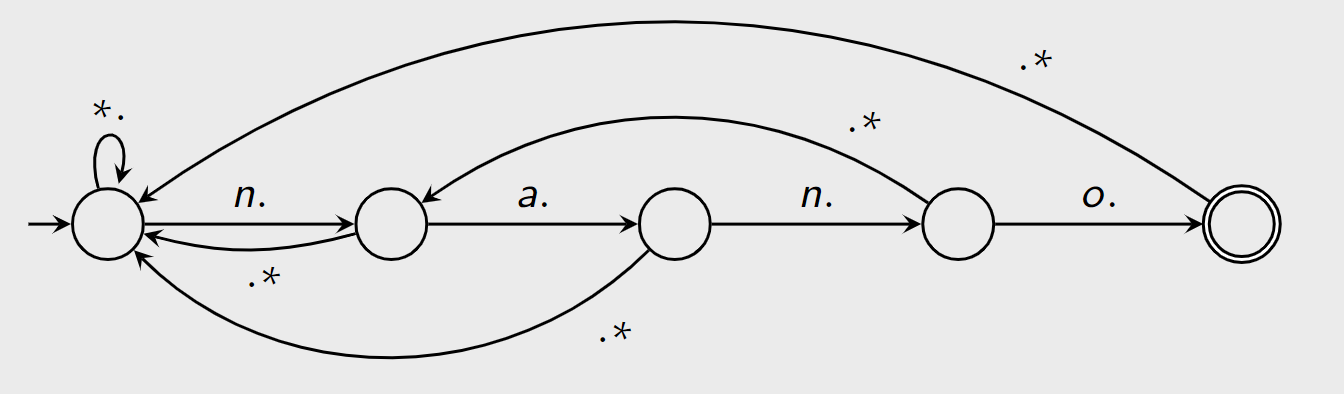
\includegraphics[scale=0.4]{img/cap3/ejemplo6_2.png}
    \end{figure}
}

\paragraph{Ejecución.} Sea $\ca{A}$ un DFA con $k$-lookahead. Tenemos que:
\begin{itemize}
    \item Un par $(q, w) \in Q \times(\Sigma \cup\{\$\})^*$ es una \textbf{configuración} de $\ca{A}$.
    \item Una configuración $(q_0, w\$^k)$ es \textbf{inicial}.
    \item Una configuración $(q, \$^k)$ es \textbf{final} si $q \in F$.
\end{itemize}

El sufijo $\$^k$ nos sirve para marcar el finald el input (y simplificar la definición de lookahead al leer el final de la palabra). \medbreak

Se define la relación $\vdash_\ca{A}$ de \textbf{siguiente-paso} entre configuraciones de $\ca{A}$:
\alignformula{
    \left(p_1, w_1\right) \vdash_\mathcal{A}\left(p_2, w_2\right)
}
si, y sólo si, $\delta\left(p_1, u . v\right)=p_2$ y existe $w \in \Sigma^*$ tal que $w_1 = uvw$ y $w_2 = vw$. \medbreak

Se define $\vdash_\ca{A}^*$ como la clausura \textbf{refleja} y transitiva de $\vdash_A$:
\alignformula{
    \text{para toda configuración } (p,w): \quad &(p,w) \vdash_\ca{A}^* (p,w) \\
    \text{si } (p_1, w_1) \vdash_\ca{A}^* \text{ y } (p2,w_2) \vdash_\ca{A} (p_3,w_3): \quad &\left(p_1, w_1\right) \vdash_{\mathcal{A}}^*\left(p_3, w_3\right)
}

Decimos que $(p,u) \vdash_\ca{A}^* (q,v)$ si uno puede ir de $(p,u)$ a $(q,v)$ en \textbf{0 o más pasos}.

\paragraph{Aceptación.} Decimos que $\ca{A}$ \textbf{acepta} $w$ si existe una configuración inicial $(q_0, w\$^k)$ y una configuración final $(q_f, \$^k)$ tal que:
$$
    \left(q_0, w \mathbb{S}^k\right) \vdash_{\mathcal{A}}^*\left(q_f, \mathbb{S}^k\right)
$$
El \textbf{lenguaje aceptado} por $\ca{A}$ se define como:
$$
    \mathcal{L}(\mathcal{A})=\left\{w \in \Sigma^* \mid \mathcal{A} \text { acepta } w\right\}
$$
Vemos que son las mismas definiciones para un $\epsilon$-NFA.

\teorema{}{}{
    Para todo DFA con $k$-lookahead $\ca{A}$ se tiene que $\ca{L}(\ca{A})$ es un \textbf{lenguaje regular}.
}
La demostración de este teorema queda como ejercicio propuesto al lector.

\paragraph{Definición.} Llamaremos un \textbf{lazy autómata} a un DFA con $1$-lookahead.

\subsubsection{Algoritmo KMP}

\paragraph{Construcción de un lazy automata.} Sea $w = w_1 \ldots w_m$ y $\mathcal{A}_w^{\mathrm{det}}=\left(Q^{\mathrm{det}}, \Sigma, \delta^{\mathrm{det}},\{0\}, F^{\mathrm{det}}\right)$ la determinización de $\ca{A}_w$.

\paragraph{Definición.} Para $i \in [0,m]$, sea $S_i$ el \textbf{único estado} en $Q^\text{det}$ tal que $i = \max(S_i)$.

\paragraph{Propiedad.} Para todo $a \in \{w_1,\ldots w_m\}$ y $i \in [0,m-1]$:
\begin{enumerate}
    \item $S_i-\{i\} \in Q^{\operatorname{det}}$
    \item $a=w_{i+1}$, entonces $\delta^{\operatorname{det}}\left(S_i, a\right)=S_{i+1}$.
    \item $a \neq w_{i+1}$, entonces $\delta^{\operatorname{det}}\left(S_i, a\right)=\delta^{\operatorname{det}}\left(S_i-\{i\}, a\right)$.
\end{enumerate}
La demostración de esta propiedad queda como ejercicio propuesto al lector. \medbreak

En base a la propiedad anterior, se define el lazy autómata $\mathcal{A}_w^{\text {lazy}}=\left(Q^{\text {det}}, \Sigma, \delta^{\text {lazy }},\{0\}, F^{\text {det }}\right)$ tal que:
\begin{itemize}
    \item para todo $a\neq w_1$: $\delta^{\text {lazy}}(\{0\}, a .)=\{0\}$.
    \item para todo $a \in \{w_1,\ldots, w_m\}$ y $i \in [0,m-1]$:
          \begin{itemize}
              \item si $a = w_{i_1}$, entonces $\delta^{\text {lazy}}\left(S_i, a_{.}\right)=S_{i+1}$
              \item si $a \neq w_{i+1}$ y $i \neq 0$, entonces $\delta^{\text {lazy}}\left(S_i, . a\right)=S_i-\{i\}$.
          \end{itemize}
\end{itemize}
\ejemplo{}{}{
    \img{img/cap3/ejemplo7.png}{0.35}
}

\teorema{}{}{
    Para todo $w$ se cumple que $\mathcal{L}\left(\mathcal{A}_w^{\text {det}}\right)=\mathcal{L}\left(\mathcal{A}_w^{\text {lazy}}\right)$.
}
La demostración queda como ejercicio propuesto para el lector (usando la propiedad).

\paragraph{Complejidad KMP.} Vemos que:
\begin{itemize}
    \item El número de pasos que $\ca{A}_w^\text{lazy}$ \textbf{consume} letras $= |d|$
    \item El número de pasos que $\ca{A}_w^\text{lazy}$ \textbf{retrocede} $\leq |d|$
    \item El número de \textbf{pasos totales} de $\ca{A}_w^\text{lazy}$ $\leq 2 \cdot |d|$
\end{itemize}
Por lo tanto, la cantidad de pasos es \textbf{lineal} en $\ca{O}(|d|)$.

\paragraph{Algoritmo KMP.} Dado una palabra $w$ y un documento $d$:
\begin{enumerate}
    \item Construimos $\ca{A}_w^\text{lazy}$ desde $\ca{A}_w$.
    \item Ejecutamos $\ca{A}_w^\text{lazy}$ sobre $d$.
\end{enumerate}

El paso 1 toma $\ca{O}(|w|)$ y el paso 2 toma $\ca{O}(|d|)$, por lo tanto, el tiempo del algoritmo es $\ca{O}(|w| + |d|)$. \medbreak

Queda como ejercicio para el lector demostrar que construir $\ca{A}_w^\text{lazy}$ toma tiempo $\ca{O}(|w|)$.





\section{Lenguajes libres de contexto}

\subsection{Gramáticas libres de contexto}

\subsubsection{Gramáticas}

\paragraph{Definición.} Una \textbf{gramática libre de contexto} (CFG) es una tupla:
\alignformula{
    \ca{G} = (V, \Sigma, P, S)
}
\begin{itemize}
    \item $V$ es un conjunto finito de \textbf{variables} o \textbf{no-terminales}.
    \item $\Sigma$ es el alfabeto finito (o \textbf{terminales}) tal que $\Sigma \cap V = \varnothing$.
    \item $P \subseteq V \times(V \cup \Sigma)^*$ es un subconjunto finito de \textbf{reglas} o \textbf{producciones}.
    \item $S \in V$ es la \textbf{variable inicial}.
\end{itemize}

\ejemplo{}{}{
    Considere la gramática $\ca{G} = (V, \Sigma, P, S)$ tal que:
    \begin{itemize}
        \item $V = \{X, Y\}$
        \item $\Sigma = \{a,b\}$
        \item $\{(X, aXb), (X, Y), (Y, \epsilon)\}$
        \item $S = X$
              \begin{align*}
                  \ca{G}: \quad  X & \to aXb      \\
                  X                & \to Y        \\
                  Y                & \to \epsilon
              \end{align*}
    \end{itemize}
}

\paragraph{Notación.} En este texto:
\begin{itemize}
    \item Para las \textbf{variables} en una gramática usaremos letras mayúsculas: $X,Y,Z,A,B,C,\ldots$
    \item Para los \textbf{terminales} en una gramática usaremos letras minúsculas: $a,b,c,\ldots$
    \item Para palabras en $(V \cup \Sigma)^*$ usaremos símbolos: $\alpha, \beta, \gamma, \ldots$
    \item Para una producción $(A,\alpha) \in P$ la escribimos como: $A \to \alpha$
\end{itemize}

\paragraph{Simplificación.} Si tenemos un conjunto de reglas de la forma:
$$
    \begin{array}{lll}
        X & \rightarrow & \alpha_1 \\
        X & \rightarrow & \alpha_2 \\
          & \cdots      &          \\
        X & \rightarrow & \alpha_n
    \end{array}
$$
entonces escribimos estas reglas \textbf{sucintamente} como
$$
    X \to \alpha_1 \mid \alpha_2 \mid \cdots \mid \alpha_n
$$
Recordando que $\alpha_1, \alpha_2, \ldots, \alpha_n \in (V \cup \Sigma)^*$.

\ejemplo{}{}{
    La gramática del ejemplo anterior:
    \begin{align*}
        \ca{G}: \quad  X & \to aXb      \\
        X                & \to Y        \\
        Y                & \to \epsilon
    \end{align*}
    Podemos escribirla en notación \textbf{sucinta} como:
    \begin{align*}
        \ca{G}: \quad X & \to aXb \mid Y \\
        Y               & \to \epsilon
    \end{align*}
}

\paragraph{Producciones.} Sea $\ca{G}$ una CFG. Definimos la relación $\Rightarrow \subseteq(V \cup \Sigma)^* \times(V \cup \Sigma)^*$ de \textbf{producción} tal que:
\alignformula{
    \alpha \cdot X \cdot \beta \Rightarrow \alpha \cdot \gamma \cdot \beta \quad \text { si, y solo si, } \quad(X \rightarrow \gamma) \in P
}
para todo $X \in V$ y $\alpha, \beta, \gamma \in(V \cup \Sigma)^*$. \medbreak

Si $\alpha X \beta \Rightarrow \alpha \gamma \beta$ entonces decimos que:
\begin{itemize}
    \item $\alpha X \beta$ \textbf{produce} $\alpha \gamma \beta$ o
    \item $\alpha \gamma \beta$ \textbf{es producible} desde $\alpha X \beta$.
    \item $\alpha X \beta \Rightarrow \alpha \gamma \beta$ es \textbf{reemplazar} $\gamma$ en $X$ en la palabra $\alpha X \beta$.
\end{itemize}

\paragraph{Derivaciones.} Sea $\ca{G}$ una CFG. Dadas dos palabras $\alpha, \beta \in(V \cup \Sigma)^*$ decimos que $\alpha$ \textbf{deriva} $\beta$:
\alignformula{
    \alpha \overunder{\Rightarrow}{}{*} \beta
}
si existe $\alpha_1, \alpha_2, \ldots, \alpha_n \in(V \cup \Sigma)^*$ tal que: $\alpha \Rightarrow \alpha_1 \Rightarrow \alpha_2 \Rightarrow \ldots \Rightarrow \beta$, con $\overunder{\Rightarrow}{}{*}$ la \textbf{clausura refleja y transitiva} de $\Rightarrow$, esto es:
\begin{enumerate}
    \item $\alpha \overunder{\Rightarrow}{}{*} \alpha$
    \item $\alpha \overunder{\Rightarrow}{}{*} \beta$ si, y sólo si, existe $\gamma$ tal que $\alpha \overunder{\Rightarrow}{}{*} \gamma$ y $\gamma \Rightarrow \beta$.
\end{enumerate}
para todo $\alpha, \beta \in (V \cup \Sigma)^*$. Notemos que $\Rightarrow$ y $\overunder{\Rightarrow}{}{*}$ son relaciones entre palabras en $(V \cup \Sigma)^*$.

\paragraph{Lenguaje.} Sea $\ca{G}$ una CFG. El \textbf{lenguaje} de una gramática $\ca{G}$ se define como:
\alignformula{
    \mathcal{L}(\mathcal{G})=\left\{w \in \Sigma^* \mid S \stackrel{\star}{\Rightarrow} w\right\}
}

$\ca{L}(\ca{G})$ son todas las palabras en $\Sigma^*$ que se pueden derivar desde $S$.

\ejemplo{}{}{
    Sea $\ca{G}$ una CFG tal que:
    \begin{align*}
        \ca{G}: \quad X & \to aXb \mid Y \\
        Y               & \to \epsilon
    \end{align*}
    \begin{itemize}
        \item Como $X \overunder{\Rightarrow}{}{*} aaabbb$, entonces $aaabbb \in \ca{L}(\ca{G})$.
        \item En general, uno puede demostrar por \textbf{inducción} que:
              $$
                  \mathcal{L}(\mathcal{G})=\left\{a^n b^n \mid n \geq 0\right\}
              $$
    \end{itemize}
}

\paragraph{Lenguaje libre de contexto.} Diremos que $L \subseteq \Sigma^*$ es un \textbf{lenguaje libre de contexto} si, y sólo si, existe una gramática libre de contexto $\ca{G}$ tal que:
\alignformula{
    L = \ca{L}(\ca{G})
}

\ejemplo{}{}{
    Los siguientes son lenguajes libres de contexto:
    \begin{itemize}
        \item $L=\left\{a^n b^n \mid n \geq 0\right\}$
        \item $\text{Par}=\left\{w \in\{a, b\}^* \mid w \text { tiene largo par }\right\}$
        \item $\text{Pal}=\left\{w \in\{a, b\}^* \mid w=w^{\mathrm{rev}}\right\}$
    \end{itemize}
}

\subsubsection{Árboles y derivaciones}

\paragraph{Definición.} El conjunto de \textbf{árboles ordenados y etiquetados} (o solo árboles) sobre etiquetas $\Sigma$ y $V$, se define recursivamente como:
\begin{itemize}
    \item $t:=a$ es un árbol para todo $a \in \Sigma$.
    \item si $t_1,\ldots, t_k$ son árboles, entonces $t:= X(t_1, \ldots, t_k)$ es un árbol para todo $X \in V$.
\end{itemize}

Para un árbol $t = X(t_1,\ldots,t_k)$ cualquiera se define:
\begin{itemize}
    \item $\texttt{raiz}(t)=X$
    \item $\texttt{hijos}(t)= t_1,\ldots,t_k$
\end{itemize}

Si $t = a$, entonces decimos que $t$ es una \textbf{hoja}, $\texttt{raiz}(t) = a$ y $\texttt{hijos}(t) = \epsilon$.

\paragraph{Definición.} Fije una CFG $\ca{G} = (V, \Sigma, P, S)$. Se define el conjunto de \textbf{árboles de derivación} recursivamente como:
\begin{itemize}
    \item Si $a \in \Sigma$, entonces $t = a$ es un árbol de derivación.
    \item Si $X \to X_1 \ldots X_k \in P$ y $t_1,\ldots,t_k$ son árboles de derivación con $\texttt{raiz}(t) = X_i$ para todo $i \leq k$, entonces $t = X(t_1,\ldots,t_k)$ es un árbol de derivación.
\end{itemize}

Decimos que $t$ es un \textbf{árbol de derivación de} $\ca{G}$ si:
\begin{enumerate}
    \item $t$ es un árbol de derivación y
    \item $\texttt{raiz}(t) = S$.
\end{enumerate}
Los árboles de derivación son todos los árboles que parten desde $S$.

\ejemplo{}{}{
    Sea $\ca{G}$ una CFG tal que:
    $$
        G: \quad E \; \to \; E + E \mid E * E \mid n
    $$
    Algunos árboles de derivación para $\ca{G}$ son:
    \img{img/cap4/ejemplo5.png}{0.45}
}

\paragraph{Definición.} Sea $\ca{G}$ una CFG y $w \in \Sigma^*$. Se define la función $\texttt{yield}$ sobre árboles, recursivamente como:
\begin{itemize}
    \item Si $t = a \in \Sigma$, entonces $\texttt{yield}(t) = a$.
    \item Si $t$ no es una hoja y $\texttt{hijos}(t) = t_1 t_2 \ldots t_k$, entonces:
          $$
              \texttt{yield}(t) =\texttt{yield}(t_1) \cdot \texttt{yield}(t_2) \cdot \ldots \cdot \texttt{yield}(t_k)
          $$
\end{itemize}

Decimos que $t$ es un \textbf{árbol de derivación de} $\ca{G}$ \textbf{para} $w$ si:
\begin{enumerate}
    \item $t$ es un árbol de derivación de $\ca{G}$ y
    \item $\texttt{yield}(t) = w$
\end{enumerate}
Lo anterior significa que las hojas de $t$ forman la palabra $w$.

\paragraph{Proposición.} Sea $\ca{G} = (V, \Sigma, P, S)$ una CFG y $w \in \Sigma^*$. Tenemos que:
$$
    w \in \mathcal{L}(\mathcal{G}) \quad \text { si, y solo si,} \quad \text{existe un árbol de derivación de } \mathcal{G} \text { para } w.
$$
Un árbol de derivación es la \textbf{representación gráfica} de una derivación.

\ejemplo{}{}{
    \vspace{-10pt}
    \img{img/cap4/ejemplo6.png}{0.4}
}

\paragraph{Definición.} Sea $\ca{G} = (V, \Sigma, P, S)$ una CFG.
\begin{itemize}
    \item Definimos la \textbf{derivación por la izquierda} $\underset{\mathrm{lm}}{\Rightarrow} \; \subseteq(V \cup \Sigma)^* \times(V \cup \Sigma)^*$:
          \alignformula{
              w \cdot X \cdot \beta \underset{\mathrm{lm}}{\Rightarrow} w \cdot \gamma \cdot \beta \quad \text { si, y solo si, } \quad X \rightarrow \gamma \in P
          }
          para todo $X \in V$, $w \in \Sigma^*$ y $\beta,\gamma \in (V \cup \Sigma)^*$.

    \item Definimos la \textbf{derivación por la derecha} $\underset{\mathrm{rm}}{\Rightarrow} \; \subseteq(V \cup \Sigma)^* \times(V \cup \Sigma)^*$:
          \alignformula{
              \alpha \cdot X \cdot w \underset{\mathrm{rm}}{\Rightarrow} \alpha \cdot \gamma \cdot w \quad \text { si, y solo si, } \quad X \rightarrow \gamma \in P
          }
          para todo $X \in V$, $w \in \Sigma^*$ y $\alpha,\gamma \in (V\cup \Sigma)^*$.
\end{itemize}

Se define $\overunder{\Rightarrow}{\mathrm{lm}}{*}$ y $\overunder{\Rightarrow}{\mathrm{rm}}{*}$ como la \textbf{clausura refleja y transitiva} de $\overunder{\Rightarrow}{\mathrm{lm}}{}$ y $\overunder{\Rightarrow}{\mathrm{rm}}{}$, respectivamente.  \medbreak

$\overunder{\Rightarrow}{\mathrm{lm}}{}$ y $\overunder{\Rightarrow}{\mathrm{rm}}{}$ solo reemplaza \textbf{a la izquierda} (leftmost) y \textbf{derecha} (rightmost).

\ejemplo{}{}{
    \vspace{-10pt}
    \img{img/cap4/ejemplo7.png}{0.4}
}

\paragraph{Proposición.} Por cada árbol de derivación, existe una \textbf{única} derivación por la izquierda y una \textbf{única} derivación por la derecha. \medbreak

Por lo tanto, desde ahora podemos hablar de \textbf{árbol de derivación y derivación (izquierda o derecha)} indistintamente.

\subsubsection{Lenguajes regulares vs libres de contexto}

\paragraph{Proposición.} Para todo lenguaje regular $L$, existe una gramática libre de contexto $\ca{G}_\ca{A}$:
\alignformula{
    L = \ca{L}(\ca{G}_\ca{A})
}

\paragraph{Idea demostración.} Dado un autómata finito determinista $\ca{A} = (Q, \Sigma, \delta, q_0, F)$, ¿cómo construimos una gramática libre de contexto? \medbreak

Defina la gramática $\ca{G}_\ca{A} = (Q, \Sigma, P_\ca{A}, q_0)$ tal que:
\begin{itemize}
    \item si $\delta(p,a) = q$, entonces $p \to aq \in P_\ca{A}$
    \item si $p \in F$, entonces $p \to \epsilon \in P_\ca{A}$
\end{itemize}

Queda como ejercicio propuesto al lector demostrar que $\ca{L}(\ca{A}) = \ca{L}(\ca{G}_\ca{A})$

\subsection{Simplificación de gramáticas}

¿Cómo podemos simplificar la siguiente gramática?
\begin{align*}
    G: \quad S \  & \to \ aAa \mid aBD \mid aBH \\
    A \           & \to \ B \mid D              \\
    B \           & \to \ aBa \mid b            \\
    C \           & \to \ aCC \mid bC           \\
    D \           & \to \ aDCa \mid CFa         \\
    F \           & \to \ aFDa \mid aab         \\
    H \           & \to \ \epsilon
\end{align*}
\begin{enumerate}
    \item Dada una variable $X$, ¿es $X$ \textbf{útil} para producir palabras?
    \item Dada una producción $p:X \to \gamma$, ¿es $p$ \textbf{útil} para producir palabras?
\end{enumerate}

\subsubsection{Eliminación de variables inútiles}

\paragraph{Definición.} Sea $\ca{G} = (V,\Sigma,P,S)$ una CFG. Diremos que una variable $X \in V$ es \textbf{útil} si existe una derivación:
\alignformula{
    S \stackrel{\star}{\Rightarrow} \alpha X \beta \stackrel{\star}{\Rightarrow} w
}
Al contrario, diremos que una variable $X$ es \textbf{inútil} si NO es útil.

\paragraph{Definición.} Para una variable $X \in V$:
\begin{enumerate}
    \item Decimos que $X$ es \textbf{alcanzable} si existe una derivación:
          \alignformula{
              S \stackrel{\star}{\Rightarrow} \alpha X \beta
          }
    \item Decimos que $X$ es \textbf{generadora} si existe una derivación:
          \alignformula{
              X \stackrel{\star}{\Rightarrow} w
          }
\end{enumerate}

\paragraph{Propiedad.} Para toda variable $X \in V - \{S\}$:
\alignformula{
    \text{existe una producción } Y \to \alpha X \beta \in P \text{ tal que } Y \in V \text{ es alcanzable} \quad \Leftrightarrow \quad X \text{ es alcanzable.}
}
La demostración de esta propiedad queda como ejercicio propuesto al lector. \medbreak

Un algoritmo para determinar si una variable es alcanzable:
\begin{algorithm}[hbt!]
    \setstretch{1.25}
    \DontPrintSemicolon
    \SetKwFunction{Falcanzables}{alcanzables}
    \SetKwProg{Fn}{Function}{:}{}
    \SetKwInOut{Input}{input}\SetKwInOut{Output}{output}
    \SetKw{Let}{let}
    \SetKw{Take}{take}
    \Input{Gramática $\ca{G}=(V,\Sigma,P,S)$}
    \Output{Conjunto $C$ de variables alcanzables}
    \Fn{\Falcanzables{$\ca{G}$}}{
        \Let $C_0 := \{S\}$

        \Let $C := \varnothing$

        \While{$C_0 \neq \varnothing$}{
            \Take $Y \in C_0$

            $C_0 := C_0 - \{Y\}$

            $C := C \cup \{Y\}$

            \ForEach{$X \in V - C$ \textit{tal que existe una regla} $\Big(Y \to \alpha X \beta\Big) \in P$}{
                $C_0 := C_0 \cup \{X\}$
            }
        }

        \Return $C$
    }
\end{algorithm}

\paragraph{Propiedad.} Para toda variable $X \in V$:
\alignformula{
    \text{existe una regla } X \to \alpha \text{ tal que todas las variables en } \alpha \text{ son generadoras} \quad \Leftrightarrow \quad X \text{ es generadora.}
}

La demostración de esta propiedad queda como ejercicio propuesto al lector. \medbreak

Un algoritmo para determinar si una variable es generadora:

\begin{algorithm}[hbt!]
    \setstretch{1.25}
    \DontPrintSemicolon
    \SetKwFunction{Falcanzables}{alcanzables}
    \SetKwProg{Fn}{Function}{:}{}
    \SetKwInOut{Input}{input}\SetKwInOut{Output}{output}
    \SetKw{Let}{let}
    \SetKw{Take}{take}
    \Input{Gramática $\ca{G}=(V,\Sigma,P,S)$}
    \Output{Conjunto $G$ de variables generadoras}
    \Fn{\Falcanzables{$\ca{G}$}}{
        \Let $G_0 := \{X \in V \mid (X \to w) \in P\}$

        \Let $G := \varnothing$

        \While{$G_0 \neq G$}{
            $G := G_0$

            \ForEach{$(X \to \alpha) \in P$}{
                \If{\textit{todas las variables en} $\alpha$ \textit{estan en} $G$}{
                    $G_0 := G_0 \cup \{X\}$
                }
            }
        }

        \Return $G$
    }
\end{algorithm}

\teorema{}{}{
    Sea $G = (V, \Sigma, P, S)$ una CFG. Sea $\ca{G}''$ una gramática creada a partir de $\ca{G}$ después de:
    \begin{itemize}
        \item eliminar todas las variables y reglas NO generadoras.
        \item eliminar todas las variables y reglas NO alcanzables.
    \end{itemize}
    Entonces, $\ca{L}(\ca{G}'') = \ca{L}(\ca{G})$ y $\ca{G}''$ no contiene variables inútiles.
}

\textbf{Nota:} Debemos respetar el orden para eliminar variables generadoras y luego las alcanzables. De hacerlo al revés, la gramática resultante puede no definir el mismo lenguaje que la inicial.

\paragraph{Demostración teorema 18.} Sea $\ca{G} = (V, \Sigma, P, S)$ una CFG. \medbreak

Sea $\ca{G}' = (V', \Sigma, P', S)$ al eliminar las variables \textbf{no generadoras} de $\ca{G}$:
$$
    \begin{aligned}
        V^{\prime} & =\{X \in V \mid \exists w.\ X \underset{\mathcal{G}}{\stackrel{\star}{\Rightarrow}} w\}                                 \\
        P^{\prime} & =\left\{X \rightarrow \alpha \in P \mid X \in V^{\prime} \wedge \alpha \in\left(V^{\prime} \cup \Sigma\right)^*\right\}
    \end{aligned}
$$

Sea $\ca{G}'' = (V'', \Sigma, P'', S)$ al eliminar las variables \textbf{no alcanzables} de $\ca{G}'$:
$$
    \begin{aligned}
        V^{\prime \prime} & =\left\{X \in V^{\prime} \mid \exists \alpha, \beta.\ S \underset{\mathcal{G}^{\prime}}{\stackrel{\star}{\Rightarrow}} \alpha X \beta\right\}  \\
        P^{\prime \prime} & =\left\{X \rightarrow \alpha \in P^{\prime} \mid X \in V^{\prime \prime} \wedge \alpha \in\left(V^{\prime \prime} \cup \Sigma\right)^*\right\}
    \end{aligned}
$$

Considere las siguientes propiedades de $\ca{G}$, $\ca{G}'$ y $\ca{G}''$:
\begin{enumerate}
    \item Para todo $\alpha \in (V \cup \Sigma)^*$, si $\alpha \overunder{\Rightarrow}{\ca{G}}{*} w$ entonces $\alpha \overunder{\Rightarrow}{\ca{G}'}{*} w$.

    \item Para todo $\alpha \in (V' \cup \Sigma)^*$, si $S \overunder{\Rightarrow}{\ca{G}'}{*} \alpha$ entonces $S \overunder{\Rightarrow}{\ca{G}''}{*} \alpha$

    \item Para todo $\alpha \in (V'' \cup \Sigma)^*$, si $\alpha \overunder{\Rightarrow}{\ca{G}'}{*} w$ entonces $\alpha \overunder{\Rightarrow}{\ca{G}''}{*} w$.
\end{enumerate}

La demostración de estas propiedades queda como ejercicio propuesto al lector. \bigbreak

\textit{Demostración $\mathcal{L}\left(\mathcal{G}^{\prime \prime}\right) \subseteq \mathcal{L}(\mathcal{G})$.} Como $V'' \subseteq V$ y $P'' \subseteq P$, entonces es trivial que $\mathcal{L}\left(\mathcal{G}^{\prime \prime}\right) \subseteq \mathcal{L}(\mathcal{G})$. \bigbreak

\textit{Demostración $\mathcal{L}(\mathcal{G}) \subseteq \mathcal{L}\left(\mathcal{G}^{\prime \prime}\right)$.} Sea $w \in \ca{L}(\ca{G})$ tal que $S \overunder{\Rightarrow}{\ca{G}}{*} w$.
\begin{itemize}
    \item Por la propiedad 1, tenemos que $S \overunder{\Rightarrow}{\ca{G}'}{*} w$.
    \item Por la propiedad 2, tenemos que $S \overunder{\Rightarrow}{\ca{G}''}{*} w$.
\end{itemize}

Por lo tanto $w \in \ca{L}(\ca{G}'')$ y concluimos que $\mathcal{L}\left(\mathcal{G}^{\prime \prime}\right) \subseteq \mathcal{L}(\mathcal{G})$. \bigbreak

\textit{Demostración variables útiles.} Queremos mostrar que para todo $X \in V''$, $X$ es \textbf{útil} en $\ca{G}''$. \bigbreak

Como $X \in V''$, entonces $S \overunder{\Rightarrow}{\ca{G}'}{*} \alpha X \beta$ para algún $\alpha, \beta \in\left(V^{\prime} \cup \Sigma\right)^*$. \medbreak

Por la propiedad 2, se tiene que: $S \overunder{\Rightarrow}{\ca{G}''}{*} \alpha X \beta$ y $\alpha, \beta \in\left(V^{\prime \prime} \cup \Sigma\right)^*$. \medbreak

Como $X \in V'$ y $\alpha,\beta \in (V' \cup \Sigma)^*$, entonces existen $u, v, w$ tal que:
$$
    \alpha \overunder{\Rightarrow}{\ca{G}}{*} u, \quad X \overunder{\Rightarrow}{\ca{G}}{*} v, \quad \beta \overunder{\Rightarrow}{\ca{G}}{*} w
$$

Por la propiedad 1, se tiene que: $\alpha \overunder{\Rightarrow}{\ca{G}'}{*} u, \quad X \overunder{\Rightarrow}{\ca{G}'}{*} v, \quad \beta \overunder{\Rightarrow}{\ca{G}'}{*} w$. \medbreak

Por la propiedad 3, se tiene que: $\alpha \overunder{\Rightarrow}{\ca{G}''}{*} u, \quad X \overunder{\Rightarrow}{\ca{G}''}{*} v, \quad \beta \overunder{\Rightarrow}{\ca{G}''}{*} w$. \medbreak

Juntando todo, $S \overunder{\Rightarrow}{\ca{G}''}{*} \alpha X \beta \overunder{\Rightarrow}{\ca{G}''}{*} uvw$ y por tanto $X$ es útil en $\ca{G}''$. \hfill $\blacksquare$

\subsubsection{Eliminación de producciones inútiles}

\paragraph{Definición.} Sea $\ca{G}$ una CFG. Decimos que:
\begin{itemize}
    \item Una producción de la forma $X \to \epsilon$ es \textbf{en vacío}.
    \item Una producción de la forma $X \to Y$ es \textbf{unitaria}.
\end{itemize}

Deseamos eliminar este tipo de producciones para simplificar nuestras gramáticas, sin embargo, debemos tener cuidado con algunos detalles.

\paragraph{Proposición.} Si $\epsilon \in \ca{L}(\ca{G})$, entonces NO se pueden borrar las producciones en vacío sin alterar el lenguaje $\ca{G}$. \medbreak

Así que, desde ahora, supondremos que $\epsilon \notin \ca{L}(\ca{G})$.

\paragraph{Definición.} Sea $\ca{G} = (V, \Sigma, P, S)$ una CFG tal que $\epsilon \notin \ca{L}(\ca{G})$. Definimos a $P^*$ como el \textbf{menor conjunto de producciones} que contiene a $P$ y \textbf{cerrado bajo} las siguientes reglas:
\begin{enumerate}
    \item Si $X \to Y \in P^*$ y $Y \to \gamma \in P^*$, entonces $X \to \gamma \in P^*$.
    \item Si $X \to \epsilon \in P^*$ y $Z \to \alpha X \beta \in P^*$, entonces $Z \to \alpha \beta \in P^*$.
\end{enumerate}
Definimos $\ca{G}^* = (V, \Sigma, P^*, S)$. Entonces:
\begin{itemize}
    \item $P^*$ es finito y
    \item $\ca{L}(\ca{G}^*) = \ca{L}(\ca{G})$.
\end{itemize}

Ahora, para cualquier palabra $w \in \ca{L}(\ca{G}^*)$, sea $\ca{T}$ un árbol de derivación de $w$ en $\ca{G}^*$ de \textbf{tamaño mínimo}. Definimos las siguientes propiedades:
\begin{enumerate}
    \item El árbol de derivación $\ca{T}$ NO usa una \textbf{producción unitaria}.
    \item El árbol de derivación $\ca{T}$ NO usa una \textbf{producción en vacío}.
\end{enumerate}

La demostración de estas propiedades se hace por contradicción: se supone que $\ca{T}$ usa una producción unitaria o en vacío y se comprueba que si ocurre esto entonces $\ca{T}$ no tiene tamaño mínimo. \bigbreak

Por la propiedad 1 y 2, tenemos que \textit{para todo $w \in \ca{L}(\ca{G}^*)$, existe una derivación de $w$ en $\ca{G}$ que NO usa producciones \textbf{en vacío} ni producciones \textbf{unitarias}}. Por lo tanto, podemos eliminar las producciones en vacío y unitarias de $\ca{G}^*$.

\teorema{}{}{
    Para toda CFG $\ca{G}$ tal que $\epsilon \notin \ca{L}(\ca{G})$, sea:
    \begin{itemize}
        \item $\ca{G}^*$ la clausura de producciones unitarias y en vacío.
        \item $\hat{\ca{G}}$ el resultado de remover toda producción unitaria o en vacío de $\ca{G}^*$.
    \end{itemize}
    Entonces, $\ca{L}(\hat{\ca{G}}) = \ca{L}(\ca{G})$ y $\hat{\ca{G}}$ no tiene producciones unitarias o en vacío.
}

Resumiendo, para eliminar las producciones en vacío y unitarias de $\ca{G}$:
\begin{itemize}
    \item construimos $\ca{G}^*$ haciendo la \textbf{clausura} de producciones unitarias y en vacío,
    \item construimos $\hat{\ca{G}}$ \textbf{removiendo} todas las producciones unitarias o en vacío de $\ca{G}^*$.
\end{itemize}
Por el resultado anterior sabemos que $\ca{L}(\hat{\ca{G}}) = \ca{L}(\ca{G})$. Es importante mencionar que es posible que $\hat{\ca{G}}$ contenga símbolos inútiles.

\subsection{Forma normal de Chomsky}

\paragraph{Definición.} Una gramática $\ca{G}$ esta en \textbf{forma normal de Chomsky} (CNF) si todas sus reglas son de la forma:
\begin{itemize}
    \item $X \to YZ$
    \item $X \to a$
\end{itemize}
\ejemplo{}{}{
    La siguiente gramática está en CNF:
    \begin{align*}
        S \  & \to \ AB \mid AC \mid SS \\
        C \  & \to \ SB                 \\
        A \  & \to a                    \\
        B \  & \to b
    \end{align*}
}
Toda gramática se puede convertir en CNF. Para facilitar el proceso, considere $\ca{G} = (V, \Sigma, P, S)$ una CFG tal que $\epsilon \notin \ca{L}(\ca{G})$.
\begin{itemize}
    \item Primero, suponga que $\ca{G}$ no contiene reglas en vacío o unitarias.
    \item Por lo tanto, todas las reglas en $\ca{G}$ son de la forma:
          \begin{itemize}
              \item $X \to \gamma \quad $ para $|\gamma| \geq 2$
              \item $X \to a$
          \end{itemize}
\end{itemize}

Los pasos para convertir $\ca{G}$ en CNF son:
\begin{enumerate}
    \item Convertir todas las reglas a la forma:
          \begin{itemize}
              \item $X \to Y_1 Y_2 \ldots Y_k$ para $k \geq 2$
              \item $X \to a$
          \end{itemize}

    \item Convertir todas las reglas a la forma:
          \begin{itemize}
              \item $X \to YZ$
              \item $X \to a$
          \end{itemize}
\end{enumerate}

Para realizar el paso 1:
\begin{itemize}
    \item Para cada $a \in \Sigma$, agregamos una nueva variable $X_a$ y una regla $X_a \to a$.
    \item Reemplazamos todas las ocurrencias antiguas de $a$ por $X_a$.
\end{itemize}

\ejemplo{}{}{
    Considere la gramática $S \to aSb \mid ab$, entonces, hacer el paso 1 termina en:
    \begin{align*}
        S \  & \to \ ASB \mid AB \\
        A \  & \to \ a           \\
        B \  & \to \ b
    \end{align*}
}

\paragraph{Correctitud.} Si $\ca{G}'$ es la gramática resultante del paso 1, entonces se cumple que $\ca{L}(\ca{G}') = \ca{L}(\ca{G})$. \bigbreak

Para realizar el paso 2, tomamos cada regla $p: X \to Y_1 Y_2 \ldots Y_k$ con $k \geq 3$ y:
\begin{itemize}
    \item Agregamos una \textbf{nueva} variable $Z$.
    \item Reemplazamos la regla $p$ por \textbf{dos reglas}:
          $$
              X \to Y_1 Z \quad \text{y} \quad Z \to Y_2 \ldots Y_k
          $$
\end{itemize}
Repetimos este paso hasta llegar a la forma normal de Chosmky.

\ejemplo{}{}{
    El resultado del paso 1 anterior es:
    \begin{align*}
        S \  & \to \ ASB \mid AB \\
        A \  & \to \ a           \\
        B \  & \to \ b
    \end{align*}
    Al realizar el paso 2, la gramática queda de la forma:
    \begin{align*}
        S \  & \to \ AZ \mid AB \\
        Z \  & \to SB           \\
        A \  & \to \ a          \\
        B \  & \to \ b
    \end{align*}
}

\paragraph{Correctitud.} Si $\ca{G}''$ es la gramática resultante del paso 2, entonces se cumple que $\ca{L}(\ca{G}'') = \ca{L}(\ca{G}')$.

\teorema{}{}{
    Sea $\ca{G} = (V, \Sigma, P, S)$ una CFG tal que $\epsilon \notin \ca{L}(\ca{G})$. Existe una gramática $\ca{G}'$ en forma normal de Chomsky tal que:
    $$
        \ca{L}(\ca{G}') = \ca{L}(\ca{G})
    $$
}

Si $\ca{G}'$ no tiene reglas unitarias ni en vacío, entonces $\ca{G}'$ es de \textbf{tamaño polinomial} con respecto a $\ca{G}$.

\subsection{Lema de bombeo para lenguajes libres de contexto}

Similarmente para los lenguajes regulares, existe un lema de bombeo para lenguajes libres de contexto. \bigbreak

Sea $L\subseteq \Sigma^*$. Si $L$ es \textbf{libre de contexto}, entonces:
\alignformula{
    (\text{LB}^\text{CFL}) \quad &\text{existe un } N > 0 \text{ tal que}\\
    &\text{para toda palabra } z \in L \text{ con } |z| \geq N \\
    &\text{existe una descomposición } z = uvwxy \\
    &\hphantom{aaaaa} \text{con } vx \neq \epsilon \text{ y } |vwx| \leq N \text{ tal que}\\
    &\text{para todo } i \geq 0,\; u \cdot v^i \cdot w \cdot x^i \cdot y \in L
}

Análogamente, para demostrar que un lenguaje $L$ NO es libre de contexto, usamos el contrapositivo del lema. \bigbreak

Sea $L \subseteq \Sigma^*$. Si:
\alignformula{
    (\neg\text{LB}^\text{CFL}) \quad &\text{para todo } N > 0 \text{ tal que}\\
    &\text{existe una palabra } z \in L \text{ con } |z| \geq N \\
    &\text{para toda descomposición } z = uvwxy \\
    &\hphantom{aaaaa} \text{con } vx \neq \epsilon \text{ y } |vwx| \leq N \text{ tal que}\\
    &\text{existe } i \geq 0,\; u \cdot v^i \cdot w \cdot x^i \cdot y \notin L\\
    &\hphantom{aaaaa} \text{entonces } L \text{ NO es libre de contexto}.
}
\paragraph{Jugando contra un demonio.} El lema de bombeo puede verse como el siguiente ``juego'':
\img{img/cap4/demonio.png}{0.3}

\ejemplo{}{}{
    Considere el lenguaje $L = \{ a^{n^2} \mid n > 0\}$
    \img{img/cap4/ejemplo11.png}{0.25}

    Ganamos ya que al bombear con $i = 2$ ya no se cumple que $j + k + l + m + n = N^2$ (se rompe el equilibrio), y entonces $z \notin L$.
}

\newpage

\ejemplo{}{}{
    Considere el lenguaje $L = \{a^n b^n c^n \mid n > 0\}$.
    \img{img/cap4/ejemplo12.png}{0.25}

    Ganamos el juego, ya que, como $uvwxy = a^N b^N c^N$ con $vx \neq \epsilon$ y $|vwx| \leq N$, entonces
    $$
        vwx \in \ca{L}(a^* b^*) \quad \text{o} \quad vwx \in \ca{L}(b^* c^*)
    $$
    \begin{itemize}
        \item Si $vwx \in \ca{L}(a^+ b^+)$, entonces:
              \begin{itemize}
                  \item $|u v^2 w x^2 y|_{a,b} > 2N$
                  \item $|u v^2 w x^2 y|_{c} = N$
              \end{itemize}
              Por lo tanto, $z' \notin L$.

        \item Si $vwx \in \ca{L}(b^+ c^+)$, entonces:
              \begin{itemize}
                  \item $|u v^2 w x^2 y|_{b,c} > 2N$
                  \item $|u v^2 w x^2 y|_{a} = N$
              \end{itemize}
              Por lo tanto, $z' \notin L$.
    \end{itemize}
    En ambos casos, $uv^2 w x^2 y \notin L$, y por tanto $L$ no es CFG.
}

\paragraph{Lema versión juego.} \textit{``Dado un lenguaje $L \subseteq \Sigma^*$, si \textbf{UNO} tiene una estrategia ganadora en el juego $(\neg\text{LB}^\text{CFL})$ para toda estrategia posible del demonio, entonces $L$ \textbf{NO} es libre de contexto''.}

\paragraph{Consecuencias.} Podemos establecer la siguiente proposición en base al lema de bombeo:
\begin{itemize}
    \item Para todos lenguajes libres de contexto $L_1$ y $L_2$, se cumple que $L_1 \cup L_2$ es un lenguaje libre de contexto.
    \item Existen lenguajes libres de contexto $L$, $L_1$ y $L_2$ tales que:
          \begin{itemize}
              \item $L_1 \cap L_2$ \textbf{NO} es un lenguaje libre de contexto.
              \item $L^C$ \textbf{NO} es un lenguaje libre de contexto.
          \end{itemize}
\end{itemize}

Para demostrar que la intersección no es libre de contexto, basta con un contraejemplo. Tomemos $L_1 = \{a^n b^n c^m \mid n\geq 0, m \geq 0\}$ y $L_2 = \{a^m b^n c^n \mid n \geq 0, m \geq 0\}$, al hacer su intersección, obtendremos el lenguaje $L = \{a^n b^n c^n \mid n \geq 0\}$, que ya vimos que no es libre de contexto. \medbreak

Queda como ejercicio propuesto para el lector demostrar que $L^C$ no es libre de contexto.

\subsection{Algoritmo CKY}

Dado un lenguaje libre de contexto $L$ y una palabra $w$, ¿cómo verificamos si $w \in L$?
\begin{itemize}
    \item Convertimos $\ca{G}$ en forma normal de Chomsky.
    \item Probamos todas las derivaciones de altura a lo más $|w| + 1$.
    \item Si encontramos una derivación retornamos $\texttt{TRUE}$.
\end{itemize}

Los pasos anteriores se conoce como el algoritmo CKY, inventado por John Cocke, Tadao Kasami y Daniel Younger. Es un algoritmo que usa \textbf{programación dinámica}, y es \textbf{cúbico} en $|w|$ y \textbf{lineal} en $|\ca{G}|$:
\alignformula{
    \text{Tiempo:}\; \ca{O}(|w|^3 \cdot |\ca{G}|)
}
Por simplicidad, asumiremos que las gramáticas que recibe el algoritmo están en \textbf{Forma Normal de Chomsky} (CNF).

\paragraph{Tabla del algoritmo CKY.} Para una palabra $w = a_1 a_2 \ldots a_n$ y una gramática $\ca{G} = (V, \Sigma, P, S)$ construimos la \textbf{tabla CKY}:

\img{img/cap4/cky1.png}{0.35}

Para todo $1 \leq 1 \leq j \leq n$ se define:
$$
    C_{i\, j} = \{X \in V \mid X \overunder{\Rightarrow}{\ca{G}}{*} a_i \ldots a_j\}
$$

\begin{multicols}{2}

    \paragraph{Paso 0 (inicial).} Para cada $i$, construimos el conjunto $C_{ii} \subseteq V$ tal que:
    $$
        C_{i\,i} = \{X \in V \mid X \to a_i \in P\}
    $$
    \img{img/cap4/cky2.png}{0.3}

    \paragraph{Paso 1.} Para cada $i$, construimos el conjunto $C_{i\, i +1} \subseteq V$ tal que:
    \begin{align*}
        C_{i\, i+1} =\; & \{X \in V \mid X \to YZ \in P \text{ para algún } \\
                        & Y \in C_{ii} \wedge Z \in C_{i+1 i+1}\}
    \end{align*}

    \img{img/cap4/cky3.png}{0.3}
\end{multicols}

\paragraph{Paso $k$ $(k > 0)$.} Para cada $i$, construimos el conjunto $C_{i\, i+k} \subseteq V$ tal que:
$$
    C_{i\, i+k} = \{ X \in V \mid \exists j \in [i,i+k].\ X \to YZ \in P \text{ para algún } Y \in C_{i\, j} \wedge Z \in C_{j+i \, i+k}\}
$$
\begin{figure}[H]
    \centering
    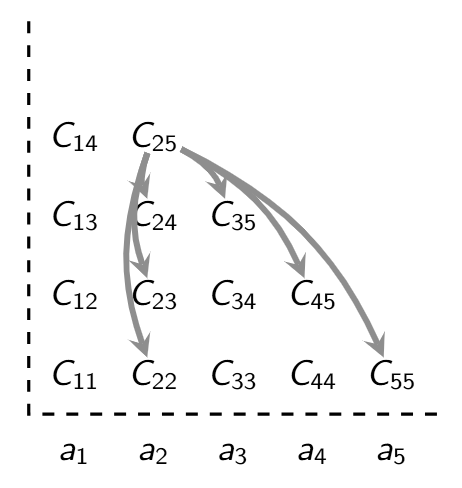
\includegraphics[scale=0.35]{img/cap4/cky4.png}
    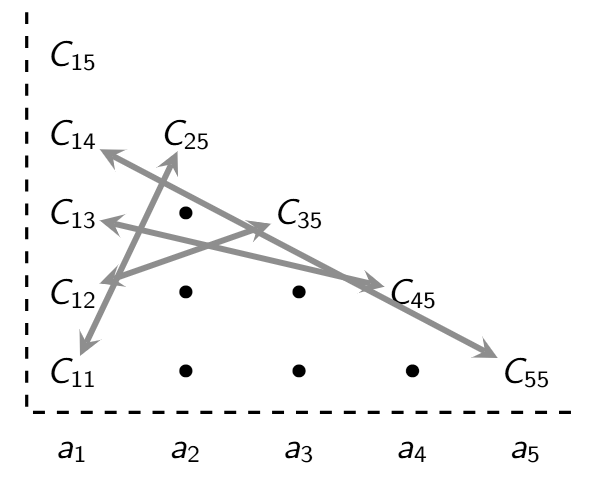
\includegraphics[scale=0.35]{img/cap4/cky5.png}
\end{figure}

\ejemplo{}{}{
    Considere la palabra $bbaba$ y la gramática:
    \img{img/cap4/ejemplo13.png}{0.6}

    Considere la palabra $abba$ y la gramática:
    \img{img/cap4/ejemplo13_1.png}{0.6}
}
\newpage
\paragraph{Algoritmo CKY.} A continuación se muestra el pseudo-código del algoritmo:

\begin{algorithm}[hbt!]
    % \caption*{An algorithm with caption}\label{alg:two}
    \setstretch{1.5}
    \DontPrintSemicolon
    \SetKwFunction{FAlgoritmoCKY}{AlgoritmoCKY}
    \SetKwProg{Fn}{Function}{:}{}
    \SetKwInOut{Input}{input}\SetKwInOut{Output}{output}
    \SetKw{Let}{let}
    \SetKw{Check}{check}
    \Input{Una gramática $\ca{G}=(V,\Sigma,P,S)$ y una palabra $w = a_1 a_2 \ldots a_n$}
    \Output{$\texttt{TRUE}$ si, y sólo si, $w \in \ca{L}(\ca{G})$}
    \Fn{\FAlgoritmoCKY{$\ca{G},w$}}{
        \For{$i = 1$ \KwTo $n$}{
            \Let $C_{i\, i} = \varnothing$

            \For{$X \to C \in P$}{
                \If{$c = a_i$}{\Let $C_{i\, i} = C_{i\, i} \cup \{X\}$}
            }
        }

        \For{$k=1$ \KwTo $n - 1$}{
            \For{$i=1$ \KwTo $n-k$}{
                \Let $C_{i\, i+k} = \varnothing$

                \For{$j = i$ \KwTo $i+k-1$}{
                    \For{$X \to YZ \in P$}{
                        \If{$Y \in C_{i\, j} \wedge Z \in C_{j+1\, i+k}$}{
                            \Let $C_{i\, i+k} = C_{i\, i+k} \cup \{X\}$
                        }
                    }
                }
            }
        }

        \Return \Check $S \in C_{1\, n}$
    }
\end{algorithm}

\paragraph{Análisis algoritmo CKY.} En su correctitud, para toda gramática $\ca{G}$ y para toda palabra $w \in \Sigma^*$ se tiene que:
$$
\texttt{AlgoritmoCKY}(\ca{G},w) = \texttt{TRUE} \quad \Leftrightarrow \quad w \in \ca{L}(\ca{G})
$$

La demostración queda como ejercicio propuesto al lector. \bigbreak

Si el input es de tamaño $|w|$ y la gramática es de tamaño $|\ca{G}|$, entonces:
$$
\text{Tiempo del algoritmo CKY:} \quad \ca{O}(|w|^3 \cdot |\ca{G}|)
$$
\section{Algoritmos para lenguajes libres de contexto}
\subsection{Autómatas apiladores}
\subsubsection{Versión normal}

\fig{img/cap5/idea_automata.png}{0.7}{Idea de un autómata apilador}

\paragraph*{Definición.} Un autómata apilador (\textit{PushDown Automata}, PDA) es una estructura:
\alignformula{
    \ca{P}=(Q,\Sigma,\Gamma,\Delta,q_0,\bot,F)
}
\begin{itemize}
    \item $Q$ es un conjunto finito de \textbf{estados}.
    \item $\Sigma$ es el alfabeto del \textbf{input}.
    \item $q_0 \in Q$ es el estado \textbf{inicial}.
    \item $F$ es el conjunto de estados \textbf{finales}.
    \item $\Gamma$ es el alfabeto de \textbf{stack}.
    \item $\bot \in \Gamma$ es el símbolo \textbf{inicial del stack} (fondo).
    \item $\Delta \subseteq(Q \times(\Sigma \cup\{\epsilon\}) \times \Gamma) \times\left(Q \times \Gamma^*\right)$ es una relación finita de transición.
\end{itemize}

Intuitivamente, la transición:
\alignformula{
    \Big((p,a,A),(q,B_1B_2\cdots B_k)\Big) \in \Delta
}
si el autómata apilador está:
\begin{itemize}
    \item en el estado $p$, leyendo $a$, y en el tope del stack hay una $A$,
\end{itemize}
entonces:
\begin{itemize}
    \item cambia al estado $q$, y modifico el tope $A$ por $B_1B_2\cdots B_k$.
\end{itemize}

Intuitivamente, la transición \textbf{en vacío}:
\alignformula{
    \Big((p,\epsilon,A),(q,B_1B_2\cdots B_k)\Big) \in \Delta
}
si el autómata apilador está:
\begin{itemize}
    \item en el estado $p$, \textit{sin lectura de una letra}, y en el tope del stack hay una $A$,
\end{itemize}
entonces:
\begin{itemize}
    \item cambia al estado $q$, y modifico el tope $A$ por $B_1B_2\cdots B_k$.
\end{itemize}

\ejemplo{}{}{
    $$
        \ca{P}=(Q,\Sigma,\Gamma,\Delta,q_0,\bot,\{q_f\})
    $$
    \begin{itemize}
        \item $Q=\{q_0,q_1,q_f\}$, $\Sigma = \{a,b\}$, $\Gamma = \{A,\bot\}$ y $\Delta$:
              $$
                  \begin{array}{ll}
                      \left(q_0, a, \perp, q_0, A \perp\right)         & q_0 \perp \stackrel{a}{\rightarrow} q_0 A \perp \\
                      \left(q_0, a, A, q_0, A A\right)                 & q_0 A \stackrel{a}{\rightarrow} q_0 A A         \\
                      \left(q_0, b, A, q_1, \epsilon\right)            & q_0 A \stackrel{b}{\rightarrow} q_1             \\
                      \left(q_1, b, A, q_1, \epsilon\right)            & q_1 A \stackrel{b}{\rightarrow} q_1             \\
                      \left(q_1, \epsilon, \perp, q_f, \epsilon\right) & q_1 \perp \stackrel{\epsilon}{\rightarrow} q_f
                  \end{array}
              $$
    \end{itemize}

    \img{img/cap5/ejemplo1.png}{0.65}
}

\paragraph*{Notación.} Dada una palabra $A_1A_2\ldots A_k \in \Gamma^+$ decimos que:
\begin{itemize}
    \item $A_1 A_2 \ldots A_k$ es un stack (contenido),
    \item $A_1$ es el \textbf{tope} del stack y
    \item $A_2 \ldots A_k$ es la \textbf{cola} del stack.
\end{itemize}

\paragraph*{Definición.} Una \textbf{configuración} de $\ca{P}$ es una tupla $(q\cdot \gamma, w) \in (Q\cdot \Gamma^*, \Sigma^*)$ tal que:
\begin{itemize}
    \item $q$ es el estado actual.
    \item $\gamma$ es el contenido del stack.
    \item $w$ es el contenido del input.
\end{itemize}
Decimos que una configuración:
\alignformula{
    (q\cdot \gamma, w) \in (Q\cdot \Gamma^*, \Sigma^*)
}
\begin{itemize}
    \item es \textbf{inicial} si $q\cdot \gamma = q_0\cdot \bot$.
    \item es \textbf{final} si $q\cdot \gamma = q_f\cdot \epsilon$ con $q_f \in F$ y $w=\epsilon$.
\end{itemize}

\paragraph*{Definición.} Se define la relación $\vdash_{\ca{P}}$ de \textbf{siguiente-paso} entre configuraciones de $\ca{P}$:
\alignformula{
    \left(q_1 \cdot \gamma_1, w_1\right) \quad \vdash_{\mathcal{P}} \quad\left(q_2 \cdot \gamma_2, w_2\right)
}
si, y sólo si, existe una transición $\left(q_1, a, A, q_2, \alpha\right) \in \Delta \text { y } \gamma \in \Gamma^*$ tal que:
\begin{itemize}
    \item $w_1 = a \cdot w_2$
    \item $\gamma_1 = A\cdot \gamma$
    \item $\gamma_2 = \alpha \cdot \gamma$
\end{itemize}

Se define $\vdash_{\ca{P}}^*$ como la clausura \textbf{refleja} y \textbf{transitiva} de $\vdash_\ca{P}$. En otras palabras:
\alignformula{
    \begin{gathered}
        \left(q_1 \gamma_1, w_1\right) \vdash_{\mathcal{P}}^*\left(q_2 \gamma_2, w_2\right) \text { si uno puede ir de }\left(q_1 \gamma_1, w_1\right) \text { a }\left(q_2 \gamma_2, w_2\right) \\
        \text { en } 0 \text { o más pasos. }
    \end{gathered}
}
\ejemplo{}{}{
    Para la palabra $w=aaabbb$, tenemos la ejecución:
    \img{img/cap5/ejemplo2.png}{0.7}
}

\paragraph*{Definiciones.} $\cal{P}$ \textbf{acepta} $w$ si, y sólo si, $\left(q_0 \perp, w\right) \vdash_{\mathcal{P}}^*\left(q_f, \epsilon\right)$ para algún $q_f \in F$.

\hspace{70pt} El \textbf{lenguaje aceptado} por $\ca{P}$ se define como:
\alignformula{
    \ca{L}(\ca{P})=\{w\in \Sigma^*\| \ \ca{P} \text{ acepta } w\}
}
\ejemplo{}{}{
    El lenguaje aceptado por el PDA utilizado en los ejemplos anteriores es $\ca{L}(\ca{P})=\{a^nb^n\ | \ n \ge 0\}$.
}

\subsubsection{Versión alternativa}
Esta definición de autómata apilador es poco común pero trae algunas ventajas:
\begin{itemize}
    \item Es un modelo que ayuda a entender mejor los algoritmos de evaluación para gramáticas.
    \item Es un modelo menos estándar pero mucho más sencillo.
    \item Al profe Cristian le gustó y lo encontró interesante.
\end{itemize}

\paragraph*{Definición.} Un \textbf{PDA alternativo} es una estructura:
\alignformula{
    \ca{D}=(Q,\Sigma,\Delta,q_0,F)
}
\begin{itemize}
    \item $Q$ es un conjunto finito de \textbf{estados}.
    \item $\Sigma$ es el alfabeto del \textbf{input}.
    \item $q_0 \in Q$ es el estado \textbf{inicial}.
    \item $F$ es el conjunto de estados \textbf{finales}.
    \item $\Delta \subseteq Q^+ \times (\Sigma \cup \{\epsilon\})\times Q^*$ es una \textbf{relación finita de transición}.
\end{itemize}
Intuitivamente, la transición:
\alignformula{
    \Big( A_1\ldots A_i, a, B_1 \ldots B_j \Big) \in \Delta
}
si el autómata apilador tiene:
\begin{itemize}
    \item $A_1\ldots A_i$ en el tope del stack y leyendo $a$,
\end{itemize}
entonces:
\begin{itemize}
    \item cambia el tope $A_1\ldots A_i$ por $B_1\ldots B_j$.
\end{itemize}

En este tipo de autómata apilador, \textbf{no hay diferencia} entre estados y alfabeto del stack.

\paragraph*{Definición.} Una \textbf{configuración} de $\ca{D}$ es una tupla
\alignformula{
    (q_1\ldots q_k, w) \in (Q^+,\Sigma^*)
}
tal que:
\begin{itemize}
    \item $q_1\ldots q_k$ es el contenido del stack con $q_1$ el tope del stack.
    \item $w$ es el contenido del input.
\end{itemize}
Decimos que una configuración:
\begin{itemize}
    \item $(q_0,w)$ es \textbf{inicial}.
    \item $(Q_f,\epsilon)$ es \textbf{final} si $q_f \in F$.
\end{itemize}

\paragraph*{Definición.} Se define la relación $\vdash_{\ca{D}}$ de \textbf{siguiente-paso} entre configuraciones de $\ca{D}$:
\alignformula{
    \left( \gamma_1, w_1\right) \quad \vdash_{\mathcal{D}} \quad\left(\gamma_2, w_2\right)
}
si, y sólo si, existe una transición $\left(\alpha, a, \beta\right) \in \Delta \text { y } \gamma \in \Gamma^*$ tal que:
\begin{itemize}
    \item $w_1 = a \cdot w_2$
    \item $\gamma_1 = \alpha\cdot \gamma$
    \item $\gamma_2 = \beta \cdot \gamma$
\end{itemize}

Se define $\vdash_{\ca{D}}^*$ como la clausura \textbf{refleja} y \textbf{transitiva} de $\vdash_\ca{D}$.

\paragraph*{Definiciones.} $\ca{D}$ \textbf{acepta} $w$ si, y sólo si, $(q_0,w) \vdash_\ca{D}^* (q_f,\epsilon)$ para algún $q_f \in F$. Además, el \textbf{lenguaje aceptado} por $\ca{D}$ se define como:
\alignformula{
    \ca{L}(\ca{D})=\{w\in \Sigma^*\| \ \ca{D} \text{ acepta } w\}
}

\newpage
\ejemplo{}{}{
    $$
        \ca{D}=(Q,\{a,b\},\Delta,q_0,F)
    $$
    \begin{itemize}
        \item $Q=\{\bot, q_0, q_1, q_f\}$ y $\Delta$:
              \img{img/cap5/ejemplo4.png}{0.6}
    \end{itemize}
    $$
        \ca{L}(\ca{D})=\{a^nb^n \ |\ n\ge 1\}
    $$
}

\teorema{}{}{
    Para todo autómata apilador $\ca{P}$ existe un autómata apilador alternativo $\ca{D}$, y viceversa, tal que:
    $$
        \ca{L}(\ca{P}) = \ca{L}(\ca{D})
    $$
}
El teorema anterior nos dice que podemos usar ambos modelos de manera \textbf{equivalente}.

\subsectionmark{PDA versus CFG}
\subsection{Autómatas apiladores vs gramáticas libres de contexto}
\subsectionmark{PDA versus CFG}
¿En qué se parecen CFG a PDA?
\fig{img/cap5/cfg_vs_pda.png}{0.3}{Gramáticas vs Autómatas apiladores}

\teorema{}{}{
    Todo \textbf{lenguaje libre de contexto} puede ser descrito equivalentemente por:
    \begin{itemize}
        \item Una gramática libre de contexto (\textbf{CFG}).
        \item Un autómata apilador (\textbf{PDA}).
    \end{itemize}
}

\subsubsection{Desde CFG a PDA}
Partimos enunciado un teorema:
\teorema{}{}{
    Para toda gramática libre de contexto $\ca{G}$, existe un \textbf{autómata apilador alternativo} $\ca{D}$, tal que:
    $$
        \ca{L}(\ca{G}) = \ca{L}(\ca{D})
    $$
}

\paragraph*{Construcción $\ca{D}$ desde $\ca{G}$.} Sea $\ca{G}=(V,\Sigma,P,S)$ una CFG. Construimos un PDA alternativo $\ca{D}$ que acepta $\ca{L}(\ca{G})$:
\alignformula{
    \ca{D}=\Big( V \cup \Sigma \cup \{q_0,q_f\}, \Sigma, \Delta, q_0, \{q_f\} \Big)
}
La relación de transición $\Delta$ se define como:
\begin{table}[H]
    \centering
    \begin{tabular}{lllll}
        $\Delta$ & $=$ & $\{ (q_0, \epsilon, S \cdot q_f) \}$               & $\cup$ &                     \\
                 &     & $\{ (X,\epsilon,\gamma)\ | \ X\to \gamma \in P \}$ & $\cup$ & \textbf{(Expandir)} \\
                 &     & $\{ (a,a,\epsilon) \ | \ a \in \Sigma \}$          &        & \textbf{(Reducir)}  \\
                 &     &                                                    &        &
    \end{tabular}
\end{table}
\paragraph*{Demostración $\ca{L}(\ca{G}) = \ca{L}(\ca{D})$.} Debemos demostrar dos direcciones: $\ca{L}(\ca{G}) \subseteq \ca{L}(\ca{D})$ y $\ca{L}(\ca{D}) \subseteq \ca{L}(\ca{G})$.

\paragraph*{Demostración $\ca{L}(\ca{G}) \subseteq \ca{L}(\ca{D})$.} Para cada $w \in \ca{L}(\ca{G})$ debemos encontrar una ejecución de aceptación de $\ca{D}$ sobre $w$. ¿Cómo encontramos esta ejecución? La idea es que para cada árbol de derivación $\ca{T}$ de $\ca{G}$ sobre $w$, construimos una ejecución de $\ca{D}$ sobre $w$ que recorre el árbol $\ca{T}$ \textbf{en profundidad} (DFS). Por tanto, debemos usar \textbf{inducción} sobre la altura del árbol $\ca{T}$.

\paragraph*{Hipótesis de inducción.} Para todo árbol de derivación $\ca{T}$ de $\ca{G}$ con \textbf{altura} $h$ tal que:
\begin{itemize}
    \item la raíz de $\ca{T}$ es $X$, y
    \item $\ca{T}$ produce la palabra $w$
\end{itemize}
entonces $(X\cdot\gamma, w) \vdash_\ca{D}^* (\gamma, \epsilon)$ para todo $\gamma \in Q^+$.

\paragraph{Caso base: $h=1$.} Si $\ca{T}$ tiene altura $1$, entonces:
\begin{itemize}
    \item $\ca{T}$ produce la palabra $w=a$ para algún $a\in \Sigma$ y
    \item $\ca{T}$ consiste de un nodo $X$ y un hijo $a$ con $X \to a$.
\end{itemize}
Entonces para todo $\gamma \in Q^+$:
$$
    (X \cdot \gamma, a) \vdash_\mathcal{D} (a \cdot \gamma, a) \vdash_\mathcal{D}(\gamma, \epsilon)
$$
es una ejecución de $\ca{D}$ sobre $a$.

\paragraph*{Caso inductivo: $h=n$.} Suponemos que el árbol de derivación $\ca{T}$ de $\ca{G}$ tiene \textbf{altura} $n$ tal que:
\begin{itemize}
    \item la raíz de $\ca{T}$ es $X$, y
    \item $\ca{T}$ produce la palabra $w$.
\end{itemize}
\textbf{Sin pérdida de generalidad}, suponga que $\ca{T}$ es de la forma:
\img{img/cap5/dem1.png}{0.5}
donde $w = u\cdot v$ y $X\to YZ$. Por HI, se tiene que para todo $\gamma_1, \gamma_2 \in Q^+$:
$$
    \begin{aligned}
        \left(Y \cdot \gamma_1, u\right) & \vdash_{\mathcal{D}}^*\left(\gamma_1, \epsilon\right) \\
        \left(Z \cdot \gamma_2, v\right) & \vdash_{\mathcal{D}}^*\left(\gamma_2, \epsilon\right)
    \end{aligned}
$$
Para $\gamma \in Q^+$ \textbf{construimos} la siguiente ejecución de $\ca{D}$ sobre $w=uv$:
$$
    (X \cdot \gamma, u v) \vdash_{\mathcal{D}}(Y Z \cdot \gamma, u v) \vdash_{\mathcal{D}}^*(Z \cdot \gamma, v) \vdash_{\mathcal{D}}^*(\gamma, \epsilon)
$$
\hfill $\blacksquare$

La demostración de $\ca{L}(\ca{D}) \subseteq \ca{L}(\ca{G})$ se deja como ejercicio propuesto al lector.

% \paragraph*{Demostración $\ca{L}(\ca{D}) \subseteq \ca{L}(\ca{G})$.} Para cada $w \in \ca{L}(\ca{D})$ debemos encontrar un árbol de derivación de $\ca{G}$ para $w$. ¿Cómo encontramos un árbol de derivación para $w$? La idea es que si tenemos una ejecución de $\ca{D}$ sobre $w$ de la forma:
% $$
%     \left(X \cdot q_f, w\right) \vdash_{\mathcal{D}}^*\left(q_f, \epsilon\right)
% $$
% entonces $X \underset{\mathcal{G}}{\stackrel{\star}{\Rightarrow}} w$. Por tanto, podemos usar \textbf{inducción} en la cantidad de pasos de la ejecución.

% \paragraph{Hipótesis de inducción.} Para toda ejecución de $\ca{D}$ sobre $w$ de largo $k$ de la forma:
% $$
%     \left(X \cdot q_f, w\right)=\left(\gamma_0, w_0\right) \vdash_\mathcal{D}\left(\gamma_1, w_1\right) \vdash_\mathcal{D} \cdots \vdash_\mathcal{D}\left(\gamma_k, w_k\right)=\left(q_f, \epsilon\right)
% $$
% entonces $X \underset{\mathcal{G}}{\stackrel{\star}{\Rightarrow}} w$.

\subsubsection{Desde PDA a CFG}
Partimos enunciando el siguiente teorema:
\teorema{}{}{
    Para todo autómata apilador $\ca{P}$, existe una gramática libre de contexto $\ca{G}$ tal que:
    $$
        \ca{L}(\ca{P}) = \ca{L}(\ca{G})
    $$
}
\paragraph{Demostración $\ca{L}(\ca{P}) = \ca{L}(\ca{G})$.} Sea $\ca{P}=(Q,\Sigma,\Gamma,\Delta,q_0,\bot,F)$ un PDA (normal). Los pasos a seguir son:
\begin{enumerate}
    \item Convertir $\ca{P}$ a un PDA $\ca{P}'$ con \textbf{UN solo estado}.
    \item Convertir $\ca{P}'$ a una gramática libre de contexto $\ca{G}$.
\end{enumerate}

\paragraph{Paso 1.} Sea $\ca{P}=(Q,\Sigma,\Gamma,\Delta,q_0,\bot,F)$ un PDA. Podemos analizar:
\begin{itemize}
    \item ¿Por qué NO necesitamos la información de los estados?
    \item ¿Cómo guardamos la información de los estados en el stack?
\end{itemize}

Esto conlleva a la siguiente pregunta: \textit{Si el PDA está en el estado $p$ y en el tope del stack hay una $A$, ¿a cuál estado llegaré al remover $A$ del stack?} \medbreak

La solución a esta pregunta es que podemos \textbf{adivinar} (no-determinismo) el estado que vamos a llegar cuando removamos $A$ del stack. \medbreak

\textbf{Sin pérdida de generalidad}, podemos asumir que
\begin{enumerate}
    \item Todas las transiciones son de la forma:
          $$
              q A \stackrel{c}{\rightarrow} p B_1 B_2 \quad \text{o} \quad q A \stackrel{c}{\rightarrow} p \epsilon
          $$
          con $c \in (\Sigma \cup \{\epsilon\})$.
    \item Existe $q_f \in Q$ tal que si $w \in \ca{L}(\ca{P})$ entonces:
          $$
              \left(q_0 \bot, w\right) \vdash_{\mathcal{D}}^*\left(q_f, \epsilon\right)
          $$
\end{enumerate}
Estos dos puntos nos aseguran  que siempre llegamos al \textbf{mismo estado} $q_f$. Luego, construimos el autómata apilador $\ca{P}'$ con \textbf{un solo estado}:
$$
    \mathcal{P}^{\prime}=\left(\{q\}, \Sigma, \Gamma^{\prime}, \Delta^{\prime},\{q\}, \perp^{\prime},\{q\}\right)
$$
\begin{itemize}
    \item $\Gamma'= Q\times \Gamma \times Q$.

          \textit{``$(p, A, q) \in \Gamma'$ si desde $p$ leyendo $A$ en el tope del stack llegamos a $q$ al hacer pop de $A$''.}

    \item $\bot' = (q_0,\bot, q_f)$.

          \textit{``El autómata parte en $q_0$ y al hacer pop de $\bot$ llegará a $q_f$''.}

    \item Si $p A \stackrel{c}{\rightarrow} p^{\prime} B_1 B_2 \in \Delta$ con $c \in (\Sigma \cup \{\epsilon\})$, entonces \textbf{para todo} $p_1,p_2 \in Q$:
          $$
              q\left(p, A, p_2\right) \stackrel{c}{\rightarrow} q\left(p^{\prime}, B_1, p_1\right)\left(p_1, B_2, p_2\right) \in \Delta^{\prime}
          $$

    \item Si $p A \stackrel{c}{\rightarrow} p^{\prime}\in \Delta$ con $c \in (\Sigma \cup \{\epsilon\})$, entonces:
          $$
              q\left(p, A, p^{\prime}\right) \stackrel{c}{\rightarrow} q \in \Delta^{\prime}
          $$
\end{itemize}

\paragraph{Hipótesis de inducción (en el número de pasos $n$).} Para todo $p,p' \in Q$, $A \in \Gamma$ y $w \in \Sigma^*$ se cumple que:
$$
    (p A, w) \vdash_{\mathcal{P}}^n\left(p^{\prime}, \epsilon\right) \quad \text { si, y solo si, } \quad\left(q\left(p, A, p^{\prime}\right), w\right) \vdash_{\mathcal{P}^{\prime}}^n(q, \epsilon)
$$
donde $\vdash_\ca{P}^n$ es la relación de \textbf{siguiente-paso} de $\ca{P}$ $n$-veces. \medbreak

Si demostramos esta hipótesis, habremos demostrado que $\ca{L}(\ca{P}) = \ca{L}(\ca{P'})$. ¿Por qué?

\paragraph{Caso base: $n=1$.} Para todo $p,p' \in Q$, y $A \in \Gamma$ se cumple que:
$$
    (p A, c) \vdash_\mathcal{P}\left(p^{\prime}, \epsilon\right) \quad \text { si, y solo si, } \quad\left(q\left(p, A, p^{\prime}\right), c\right) \vdash_{\mathcal{P}^{\prime}}(q, \epsilon)
$$
para todo $c \in (\Sigma \cup \{\epsilon\})$.

\paragraph{Caso inductivo.} \textbf{Sin pérdida de generalidad}, suponga que $pA \overset{a}{\to} p_1A_1A_2$ y $w=auv$, entonces

$$
    (p A, \underbrace{a u v}_w) \vdash_{\mathcal{P}}^n\left(p^{\prime}, \epsilon\right) \text { ssi }(p A, a u v) \vdash_{\mathcal{P}}\left(p_1 A_1 A_2, u v\right) \vdash_{\mathcal{P}}^i\left(p_2 A_2, v\right) \vdash_{\mathcal{P}}^j\left(p^{\prime}, \epsilon\right)
$$
\begin{align*}
     & \text{ssi }  \left(p_1 A_1, u\right) \vdash_{\mathcal{P}}^i\left(p_2, \epsilon\right) \text { y } \quad\left(p_2 A_2, v\right) \vdash_{\mathcal{P}}^j\left(p^{\prime}, \epsilon\right)                                  \\
     & \text {ssi }  \left(q\left(p_1, A_1, p_2\right), u\right) \vdash_{\mathcal{P}^{\prime}}^i(q, \epsilon) \text { y } \quad\left(q\left(p_2, A_2, p^{\prime}\right), v\right) \vdash_{\mathcal{P}^{\prime}}^j(q, \epsilon) \\
     & \text {ssi }  \left.\left(q\left(p, A, p^{\prime}\right), auv\right) \vdash_{\mathcal{P}}\left(q\left(p_1, A_1, p_2\right)\left(p_2, A_2, q\right)\right), u v\right) \vdash_{\mathcal{P}}^{i+j}(q, \epsilon)
\end{align*}

\hfill $\blacksquare$

\paragraph{Paso 2.} Sea $\ca{P}=(\{q\},\Sigma,\Gamma,\Delta,q,\bot,\{q\})$ un PDA con \textbf{UN solo estado}. Construimos la gramática:
$$
    \ca{G} = (V, \Sigma, P, \bot)
$$
\begin{itemize}
    \item $V=\Gamma$.
    \item Si $qA \overset{\epsilon}{\to} q\alpha \in \Delta$ entonces $A \to \alpha \in P$
    \item Si $qA \overset{a}{\to} q\alpha \in \Delta$ entonces $A \to a\alpha \in P$
\end{itemize}
La demostración de este paso queda como ejercicio propuesto al lector.

\subsection{Parsing: cómputo de First y Follow}

\paragraph{Recordatorio.} La \textbf{sintaxis} de un lenguaje es un conjunto de reglas que describen los programas válidos que tienen significado. Por otro lado, la \textbf{semántica} de un lenguaje define el significado de un programa correcto según la sintaxis.
\fig{img/cap5/parsing.png}{0.3}{La estructura de un compilador}

Lo que se busca es un proceso de \textbf{verificación de sintaxis} de un programa, y que entregue la estructura del mismo (árbol de parsing). Consta de tres etapas:
\begin{enumerate}
    \item Análisis léxico (\textbf{Lexer}).
    \item Análisis sintático (\textbf{Parser}).
    \item Análisis semántico.
\end{enumerate}
En una sección anterior vimos el \textbf{Lexer}. Ahora, veremos como hacer el \textbf{Parser}. \medbreak

Informalmente: \textit{``dado una secuencia de tokens $w'$ y una gramática $\ca{G}$, construir un árbol de derivación (parsing) de $\ca{G}$ para $w$''.} \medbreak

Con el \textbf{árbol de derivación} habremos verificado la sintaxis y obtenido la estructura.

\newpage

\ejemplo{Parsing de gramática}{}{
    $$
        E \ \rightarrow \ (E+E)\ |\ (E * E)\ |\ \text {num}
    $$
    Para un input $w = ((43+56)*27)$:
    \begin{itemize}
        \item Convertimos $w$ en una secuencia de \textbf{tokens}:
              $$
                  w'=((\text{num} + \text{num})*\text{num})
              $$
        \item Construimos un árbol de \textbf{parsing} para $w'$:
              \img{img/cap5/ejemplo5.png}{0.5}
    \end{itemize}
}

\paragraph{Problema de parsing.} Dado una palabra $w$ y dado una gramática $\ca{G}$, generar un árbol de parsing $\ca{T}$ de $\ca{G}$ para $w$. ¿Ya sabemos resolver este problema? El algoritmo CKY nos permite hacer esto, pero:
\begin{itemize}
    \item es impracticable para grandes inputs.
    \item múltiples pasadas sobre el input.
\end{itemize}
Deseamos hacer parsing en \textbf{tiempo lineal} en el tamaño del input. ¿Quién nos puede rescatar ante tal problema? Efectivamente, los autómatas apiladores. \medbreak

Recordemos que, para una gramática $\ca{G}=(V,\Sigma, P, S)$ \textbf{podemos construir un PDA alternativo} $\ca{D}$ que acepta $\ca{L}(\ca{G})$:
$$
    \ca{D}=\Big( V \cup \Sigma \cup \{q_0,q_f\}, \Sigma, \Delta, q_0, \{q_f\} \Big)
$$
La relación de transición $\Delta$ se define como:
\begin{table}[H]
    \centering
    \begin{tabular}{lllll}
        $\Delta$ & $=$ & $\{ (q_0, \epsilon, S \cdot q_f) \}$               & $\cup$ &                     \\
                 &     & $\{ (X,\epsilon,\gamma)\ | \ X\to \gamma \in P \}$ & $\cup$ & \textbf{(Expandir)} \\
                 &     & $\{ (a,a,\epsilon) \ | \ a \in \Sigma \}$          &        & \textbf{(Reducir)}  \\
                 &     &                                                    &        &
    \end{tabular}
\end{table}
Con esto, nos encontramos con otro \textbf{problema}: hay muchas alternativas para \textbf{expandir}. ¿Cómo elegir entonces la siguiente producción para expandir? Por ejemplo, si tenemos la regla $X \to \alpha \ | \ \beta$, ¿cómo elegir entre $\alpha$ o $\beta$? \medbreak

Queremos elegir la \textbf{próxima producción} $X\to\gamma$ de tal manera que, si existe una derivación para el input, entonces $X\to\gamma$ \textbf{es parte de esa derivación}:
$$
    \text { si }\quad  S \underset{\mathrm{lm}}{\stackrel{\star}{\Rightarrow}} u X \gamma^{\prime} \underset{\mathrm{lm}}{\stackrel{\star}{\Rightarrow}} u v, \text { entonces}\quad \gamma \gamma^{\prime} \underset{\mathrm{lm}}{\stackrel{\star}{\Rightarrow}} v
$$
Necesitamos \textbf{mirar las siguientes letras en} $v$ y ver si pueden ser producidas por $\alpha$ o $\beta$. Para esto, ocuparemos los conceptos de \textbf{first} y \textbf{follow}.

\subsubsection{Prefijos}\label{prefijos}
\paragraph{Definición.} Sea $\Sigma$ un alfabeto finito. Para un $k \ge 0$, se define
\alignformula{
    \Sigma^{\leq k}&=\bigcup_{i=0}^k \Sigma^i \\
    \Sigma_{\#}^{\leq k}&=\Sigma^{\leq k} \cup\left(\Sigma^{\leq k-1} \cdot\{\#\}\right)
}
\ejemplo{}{}{
    Para $\Sigma=\{a,b\}$:
    \begin{itemize}
        \item $\Sigma^{\le 2}=\{\epsilon, a, b, aa, ab, ba, bb\}$
        \item $\Sigma_{\#}^{\le 2}=\{\epsilon,a,b,aa,ab,ba,bb\}\cup \{\#,a\#,b\#\}$
    \end{itemize}
}
El símbolo $\#$ representará un EOF (End Of File), marcando el \textbf{fin de una palabra}.

\paragraph{Definición.} Para una palabra $w=a_1a_2\ldots a_n \in \Sigma^*$ se define el $k$-\textbf{prefijo} de $w$ como:
\alignformula{
    \left.w\right|_k= \begin{cases}a_1 \ldots a_n & \text { si } n \leq k \\ a_1 \ldots a_k & \text { si } k<n\end{cases}
}
Definimos la $k$-\textbf{concatenación} $\odot_k$ entre strings $u,v \in \Sigma$ como:
\alignformula{
    u \odot_k v=\left.(u \cdot v)\right|_k
}
\ejemplo{}{}{
    Sea $\Sigma = \{a,b\}$, entonces:
    \begin{itemize}
        \item $(abaa)|_2 = ab \qquad (ab)|_2 = ab \qquad (a)|_2=a \qquad (\epsilon)|_2=\epsilon$
        \item $a \odot_2 baa = (abaa)|_2 = ab$
        \item $bba \odot_2 a = (bbaa)|_2 = bb$
        \item $b \odot_2 \epsilon = (b)|_2 = b$
    \end{itemize}
}

Extendemos estas operaciones para lenguajes $L,L_1,L_2 \subseteq \Sigma^*$ como:
\alignformula{
    L|_k &=\left\{\left.w\right|_k \mid w \in L\right\} \\
    L_1 \odot_k L_2 &=\left\{w_1 \odot_k w_2 \mid w_1 \in L_1 \text{ y } w_2 \in L_2\right\}
}

\ejemplo{}{}{
    \begin{itemize}
        \item $((ab)^*)|_3 = \{\epsilon, ab, aba\}$
        \item $(a)^* \odot_3 (ab)^* = \{\epsilon, a, aa, aaa, ab, aba, aab\}$
    \end{itemize}
}
Podemos decir que los operadores $|_k$ y $\odot_k$ ``miran'' hasta un prefijo $k$.

\paragraph{Propiedades.} Para todo $k\ge 1$ y $L_1,L_2,L_3 \subseteq \Sigma^*$:
\begin{enumerate}
    \item $L_1 \odot_k (L_2 \odot_k L_3) = (L_1 \odot_k L_2) \odot_k L_3$
    \item $L_1 \odot_k \{\epsilon\} = \{\epsilon\} \odot_k L_1 = L_1|_k$
    \item $(L_1 L_2)|_k = L_1|_k \odot_k L_2|_k$
    \item $L_1 \odot_k (L_2 \cup L_3) = (L_1 \odot_k L_2) \cup (L_1 \odot_k L_3)$
\end{enumerate}
La demostración de estas propiedades queda como ejercicio propuesto al lector.

\subsubsection{First y Follow}
Sea $\ca{G}=(V,\Sigma,P,S)$ una gramática libre de contexto y $k\ge 1$.

\paragraph{Definición.} Se define la función $\texttt{first}_k:(V\cup \Sigma)^* \to 2^{\Sigma^{\le k}}$ tal que, para $\gamma \in (V \cup \Sigma)^*$:
\alignformula{
    \texttt{first}_k(\gamma) = \{u|_k \mid \gamma \overset{*}{\Rightarrow} u\}
}
\ejemplo{}{}{
    $$
        E \quad \to \quad (E + E) \mid (E * E) \mid n
    $$
    \begin{itemize}
        \item $\texttt{first}_1(E)=\{(,n\}$
        \item $\texttt{first}_2(E)=\{n, (n, ((\}$
        \item $\texttt{first}_3(E)=\{n, (n+, (n*, ((n, (((\}$
    \end{itemize}
}

\paragraph{Definición.} Se define la función $\texttt{follow}_k:V \to 2^{\Sigma_{\#}^{\le k}}$ como:
\alignformula{
    \texttt{follow}_k(X)=\{w \mid S \overset{*}{\Rightarrow} \alpha X \beta \text{ y } w \in \texttt{first}_k(\beta \#)\}
}
\ejemplo{}{}{
    $$
        E \quad \to \quad (E + E) \mid (E * E) \mid n
    $$
    \begin{itemize}
        \item $\texttt{follow}_1(E)=\{\#,+,*,)\}$
        \item $\texttt{follow}_2(E)=\{\#, )\#, )), )+, )*, +(, *(, +n, *n\}$
    \end{itemize}
}
\fig{img/cap5/first_follow.png}{0.5}{Representación de $\texttt{first}$ y $\texttt{follow}$}

\subsubsection{Calcular First}
Sea $\ca{G}=(V,\Sigma,P,S)$ una gramática libre de contexto y $k\ge 1$.
\paragraph{Proposición.} Para $X_1, \ldots, X_n \in (V\cup \Sigma)$:
\alignformula{
    \texttt{first}_k\left(X_1 \ldots X_n\right)=\texttt{first}_k\left(X_1\right) \odot_k \cdots \odot_k \texttt{first}_k\left(X_n\right)
}
\paragraph{Demostración.} Defina $\ca{L}(X)=\{w \mid X \overset{*}{\Rightarrow} w\}$ y $\ca{L}(\gamma) = \{w \mid \gamma \overset{*}{\Rightarrow} w\}$. Notar que $\texttt{first}_k(\gamma) = \ca{L}(\gamma)|_k$, por lo tanto, tenemos que
\begin{align*}
    \texttt{first}_k\left(X_1 \ldots X_n\right) & =\left.\mathcal{L}\left(X_1 \ldots X_n\right)\right|_k                                                                                    \\
                                                & =\left.\left(\mathcal{L}\left(X_1\right) \cdot \mathcal{L}\left(X_2\right) \cdot \ldots \cdot \mathcal{L}\left(X_n\right)\right)\right|_k \\
                                                & =\mathcal{L}\left(X_1\right)_k \odot_k \mathcal{L}\left(X_2\right)_k \odot_k \ldots \odot_k \mathcal{L}\left(X_n\right)|_k                \\
                                                & =\texttt{first}_k\left(X_1\right) \odot_k \cdots \odot_k \texttt{first}_k\left(X_n\right)
\end{align*}
\hfill $\blacksquare$ \medbreak

En particular, tenemos que:
\alignformula{
    \texttt{first}_k(X) = \bigcup_{X\to X_1\ldots X_n \in P} \texttt{first}_k(X_1) \odot_k \cdots \odot_k \texttt{first}_k(X_n)
}

Definimos el siguiente \textbf{programa recursivo} para todo $X \in (V \cup \Sigma)$:
\begin{align*}
    \texttt{first}_k^0(X) & :=\bigcup_{X \rightarrow w \in P} w|_k                                                                                                              \\
    \texttt{first}_k^i(X) & :=\bigcup_{X \rightarrow X_1 \ldots X_n \in P} \texttt{first}_k^{i-1}\left(X_1\right) \odot_k \cdots \odot_k \texttt{first}_k^{i-1}\left(X_n\right) \\
\end{align*}
Es fácil ver que:
\begin{itemize}
    \item $\texttt{first}_k^{i-1}(X) \subseteq \texttt{first}_k^i(X)$ para todo $i > 1$.
    \item Como $\texttt{first}_k(X) \subseteq \Sigma^{\le k}$, entonces para algún $i \le k \cdot |\Sigma|^k \cdot |V|$ tendremos:
          $$
              \texttt{first}_k^j(X)=\texttt{first}_k^{j+1}(X) \text { para todo } j \geq i
          $$
\end{itemize}

\teorema{}{}{
    Sea $i^*$ el menor número tal que $\first_k^{i^*}(X) = \first_k^{i^*+1}(X)$ para todo $X \in V$. Entonces, para todo $X \in V$:
    $$
        \first_k^{i^*}(X) = \first_k(X)
    $$
}
La demostración del teorema anterior queda como ejercicio propuesto para el lector. Una idea para la dirección $\subseteq$, es demostrar por inducción que $\first_k^i(X) \subseteq \first_k(X)$. Para la dirección $\supseteq$, una idea es demostrar por inducción que si $X \overset{*}{\Rightarrow} w$, entonces $w|_k \in \first_k^i(X)$ para algún $i$.

\paragraph{Algoritmo.} A continuación se presenta un algoritmo para calcular $\first_k$:
\begin{itemize}
    \item \textbf{Input:} Gramática $\ca{G}=(V,\Sigma, P, S)$ y $k\ge 1$.
    \item \textbf{Output:} Todos los conjuntos $\first_k$(X) para todo $X \in (V\cup\Sigma)$.
\end{itemize}
% \RestyleAlgo{ruled}
\vspace{-15pt}
\begin{algorithm}[hbt!]
    % \caption*{An algorithm with caption}\label{alg:two}
    \setstretch{1.25}
    \DontPrintSemicolon
    \SetKwFunction{FCalcularFirst}{CalcularFirst}
    \SetKwProg{Fn}{Function}{:}{}
    \Fn{\FCalcularFirst{$\ca{G}, k$}}{
    \ForEach{$a \in \Sigma$}{
        $\first_k^0(a) := \{a\}$
    }
    \ForEach{$X \in V$}{
        $\first_k^0(X):= \cup_{X\to w \in P}\ w|_k$
    }
    $i:=0$

    \Repeat{\textup{$\first_k^i(X) = \first_k^{i-1}(X)$ para todo $X \in (V\cup \Sigma)$}}{
        $i:=i+1$

        \ForEach{$a \in \Sigma$}{
            $\first_k^i(a) := \{a\}$
        }
        \ForEach{$X \in V$}{
            $\displaystyle{\first_k^i(X):=\bigcup_{X \rightarrow X_1 \ldots X_n \in P} \first_k^{i-1}\left(X_1\right) \odot_k \cdots \odot_k \first_k^{i-1}\left(X_n\right)}$
        }
    }
    \Return{\textup{$\{\first_k(X)\}_{X \in (V\cup\Sigma)}$}}
    }
\end{algorithm}
\vspace{-15pt}

\subsubsection{Calcular Follow}
Sea $\ca{G}=(V,\Sigma,P,S)$ una gramática libre de contexto y $k\ge 1$.
% $$
%     \texttt{follow}_k(X)=\{w \mid S \overset{*}{\Rightarrow} \alpha X \beta \text{ y } w \in \texttt{first}_k(\beta \#)\}
% $$
Si consideramos $X\neq S$:
\begin{align*}
    \follow_k(X) & =\bigcup_{S \stackrel{\star}{\Rightarrow} \alpha X \beta} \first_k(\beta \#)                                                                                                      \\
                 & =\bigcup_{S \stackrel{\star}{\Rightarrow} \alpha Y \beta \Rightarrow \alpha \alpha^{\prime} X \beta^{\prime} \beta} \first_k\left(\beta^{\prime} \beta \#\right)                  \\
                 & =\bigcup_{Y \rightarrow \alpha^{\prime} X \beta^{\prime}} \bigcup_{S \overset{*}{\Rightarrow}\alpha Y \beta} \first_k\left(\beta^{\prime} \beta \#\right)                         \\
                 & =\bigcup_{Y \rightarrow \alpha^{\prime} X \beta^{\prime}} \bigcup_{S \stackrel{\star}{\Rightarrow} \alpha Y \beta} \first_k\left(\beta^{\prime}\right) \odot_k \first_k(\beta \#) \\
                 & =\bigcup_{Y \rightarrow \alpha^{\prime} X \beta^{\prime}} \first_k\left(\beta^{\prime}\right) \odot_k \bigcup_{S \stackrel{*}{\Rightarrow} \alpha Y \beta} \first_k(\beta \#)     \\
                 & =\bigcup_{Y \rightarrow \alpha^{\prime} X \beta^{\prime}} \first{ }_k\left(\beta^{\prime}\right) \odot_k \follow_k(Y)                                                             \\
                 &
\end{align*}

Si consideramos $X = S$:
\begin{align*}
    \follow_k(S) & =\{\#\} \cup \bigcup_{S\stackrel{+}{\Rightarrow} \alpha S \beta} \first_k(\beta \#)                                                                                          \\
                 & =\{\#\} \cup \bigcup_{S \stackrel{\star}{\Rightarrow} \alpha Y \beta \Rightarrow \alpha \alpha^{\prime} S \beta^{\prime} \beta} \first_k\left(\beta^{\prime} \beta \#\right) \\
                 & =\{\#\} \cup \bigcup_{Y \rightarrow \alpha^{\prime} S \beta^{\prime}} \first{ }_k\left(\beta^{\prime}\right) \odot_k \follow_k(Y)                                            \\
                 &
\end{align*}
Dado lo anterior, podemos definir el siguiente teorema.
\teorema{}{}{
    Sea $\ca{G}=(V,\Sigma,P,S)$ una gramática libre de contexto y $k\ge 1$. Entonces:
    \begin{align*}
         & \text { Para } X \neq S: & \follow_k(X) & =\bigcup_{Y \rightarrow \alpha X \beta} \first_k(\beta) \odot_k \follow_k(Y)                       \\
         & \text { Para } X = S:    & \follow_k(S) & =\{\#\} \cup \underset{Y \rightarrow \alpha S \beta}{\bigcup} \first_k(\beta) \odot_k \follow_k(Y)
    \end{align*}
}
Definimos el siguiente \textbf{programa recursivo} para todo $X \in V$:
\begin{table}[H]
    \centering
    \begin{tabular}{llll}
        Para $X \neq S$: & $\follow_k^0(X)$ & $:=$ & $\varnothing$                                                                                                            \\
        Para $X = S$:    & $\follow_k^0(S)$ & $:=$ & $\{\#\}$                                                                                                                 \\
        Para $X \neq S$: & $\follow_k^i(X)$ & $:=$ & $\displaystyle{\bigcup_{Y \rightarrow \alpha X \beta} \first_k(\beta) \odot_k \follow_k^{i-1}(Y)}$                       \\
        Para $X = S$:    & $\follow_k^i(S)$ & $:=$ & $\displaystyle{\{\#\} \cup \underset{Y \rightarrow \alpha S \beta}{\bigcup} \first_k(\beta) \odot_k \follow_k^{i-1}(Y)}$
    \end{tabular}
\end{table}
Similar al caso de $\first_k$, es fácil ver que:
\begin{itemize}
    \item $\follow_k^{i-1}(X) \subseteq \follow_k^i(X)$ para todo $i > 1$.
    \item Como $\follow_k(X) \subseteq \Sigma^{\le k}$, entonces para algún $i \le k \cdot |\Sigma|^k \cdot |V|$:
          $$
              \follow_k^j(X)=\follow_k^{j+1}(X) \ \text{ para todo } j \ge i
          $$
\end{itemize}
\teorema{}{}{
    Sea $i^*$ el menor número tal que $\follow_k^{i^*}(X) = \follow_k^{i^*+1}(X)$ para todo $X \in V$. Entonces, para todo $X \in V$:
    $$
        \follow_k^{i^*}(X) = \follow_k(X)
    $$
}
La demostración de este teorema se deja como ejercicio propuesto al lector. \medbreak

Con todo lo anterior, podemos calcular $\follow_k(X)$ con un algoritmo similar que $\first_k(X)$. Respecto a la eficiencia de este tipo de algoritmos:
\begin{itemize}
    \item Toman $\ca{O}(k\cdot |\Sigma|^k\cdot|V|)$ en el peor caso.
    \item Si $k = 1$, el número de repeticiones será $\ca{O}(|\Sigma|\cdot |V|)$ y el tiempo del algoritmo será polinomial en $|\ca{G}|$ en el peor caso. Incluso, se puede hacer en tiempo $\ca{O}(|V|\cdot |P|)$ en total.
\end{itemize}

\subsection{Gramáticas LL}
Volvamos a la idea de buscar un algoritmo que haga parsing en \textbf{tiempo lineal}. Para esto, contruíamos un autómata apilador alternativo $\ca{D}$ al cual le expandíamos sus producciones. ¿El problema? No sabemos como elegir que producciones expandir. Debido a lo anterior, introducimos los conceptos de $\first$ y $\follow$. Así que, si tenemos una producción de la forma $X \to \alpha \mid \beta$, ¿cómo elegir entre $\alpha$ o $\beta$?

\paragraph{Estrategia (intuición).} La idea es la siguiente:
\begin{enumerate}
    \item Mirar $k$ símbolos del resto del input $v$ ($k$-\textbf{lookahead}).
    \item Usar $v|_k$ y decidir cuál regla $X\to \gamma$ elegimos para expandir.
\end{enumerate}
La caracterización de las gramáticas que cumplen las propiedades anteriores se denominan \textbf{Gramáticas} LL($k$), donde
\begin{itemize}
    \item \textbf{Primera} L: leer el input de izquierda a derecha (\textbf{L}eft-right).
    \item \textbf{Segunda} L: producir una derivación por la izquierda (\textbf{L}eftmost).
    \item \textbf{Parámetro} $k$: el número de letras en adelante que utiliza (\textbf{lookahead}).
\end{itemize}

\subsubsection{Definición Gramáticas LL}
Sea $\ca{G}=(V,\Sigma,P,S)$ una gramática libre de contexto y $k \ge 1$.

\paragraph{Definición.} Decimos que $\ca{G}$ es una gramática $\gll(k)$ si para todas las derivaciones:
\begin{itemize}
    \item $S \ \overunder{\Rightarrow}{\mathrm{lm}}{*} \ uY\beta \ \overunder{\Rightarrow}{\mathrm{lm}}{} \ u \gamma_1 \beta \ \overunder{\Rightarrow}{\mathrm{lm}}{*} \ u v_1$
    \item $S \ \overunder{\Rightarrow}{\mathrm{lm}}{*} \ uY\beta \ \overunder{\Rightarrow}{\mathrm{lm}}{} \ u \gamma_2 \beta \ \overunder{\Rightarrow}{\mathrm{lm}}{*} \ u v_2\ $ y
    \item $v_1|_k = v_2|_k$
\end{itemize}
entonces se cumple que $\gamma_1 = \gamma_2$. \medbreak

Notar que la elección de $Y\to \gamma$ depende de $Y$, $v|_k$ y $u$.
\ejemplo{Gramáticas $\gll(1)$}{}{
    \img{img/cap5/ejemplo11.png}{0.4}
    \begin{itemize}
        \item Si $v_1|_1 = v_2|_1 = n$, entonces $\gamma_1 = \gamma_2 = n$.
        \item Si $v_1|_1 = v_2|_1 = ($, entonces $\gamma_1 = \gamma_2 = (S)$.
    \end{itemize}
    En ambos casos, tenemos que $\gamma_1 = \gamma_2$ y $\ca{G}_1$ es una gramática $\gll(1)$.
    \img{img/cap5/ejemplo12.png}{0.4}
    \begin{itemize}
        \item Si $v_1|_1 = v_2|_1 = ($ o `$n$', entonces $\gamma_1 = \gamma_2 = SX$.
        \item Si $v_1|_1 = v_2|_1 =\ )$, entonces $\gamma_1 = \gamma_2 = \epsilon$.
    \end{itemize}
    Por lo tanto, tenemos que $\gamma_1 = \gamma_2$ y $\ca{G}_2$ es \textbf{también} una gramática $\gll(1)$.
}

% \ejemplo{Gramática $\gll(1)$}{}{

% }

\ejemplo{Gramática NO $\gll(1)$ pero si $\gll(2)$}{}{
    \begin{figure}[H]
        \centering
        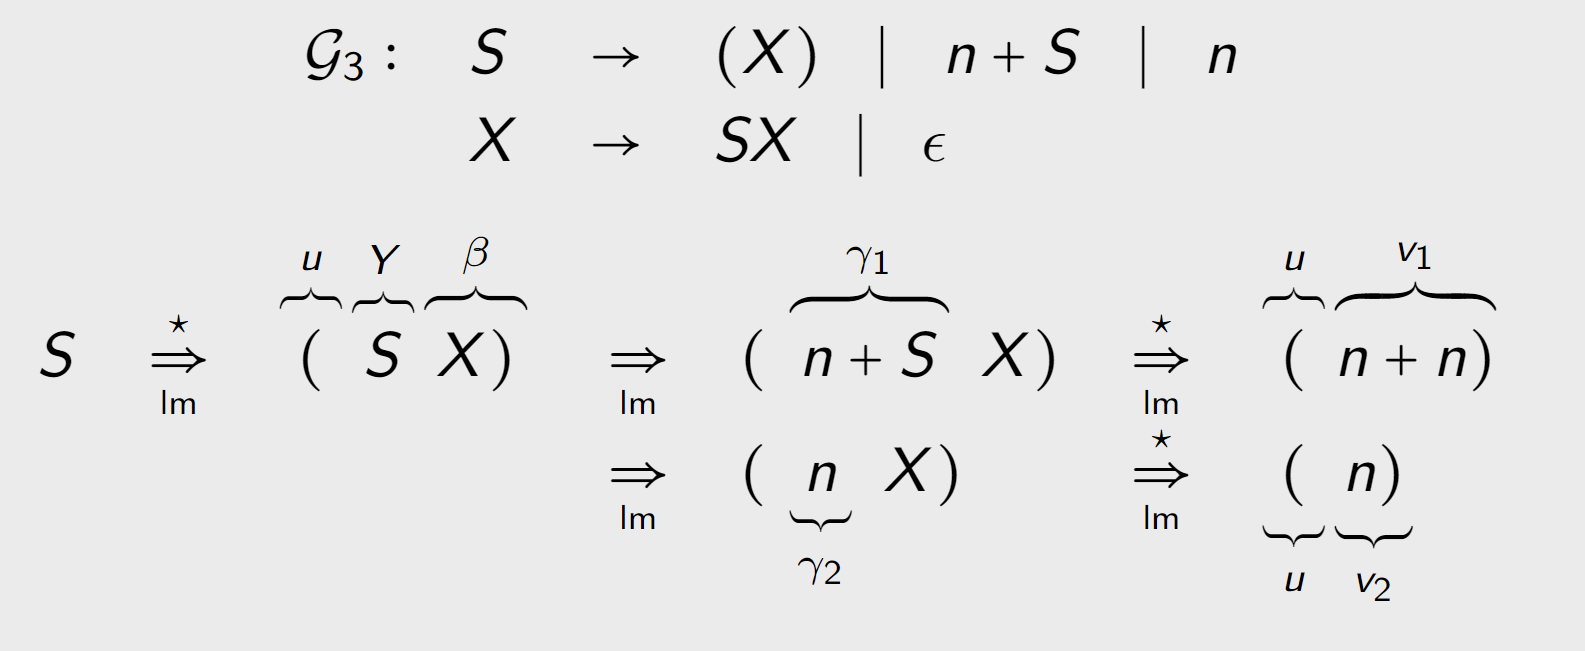
\includegraphics[scale=0.3]{img/cap5/ejemplo13.png}
        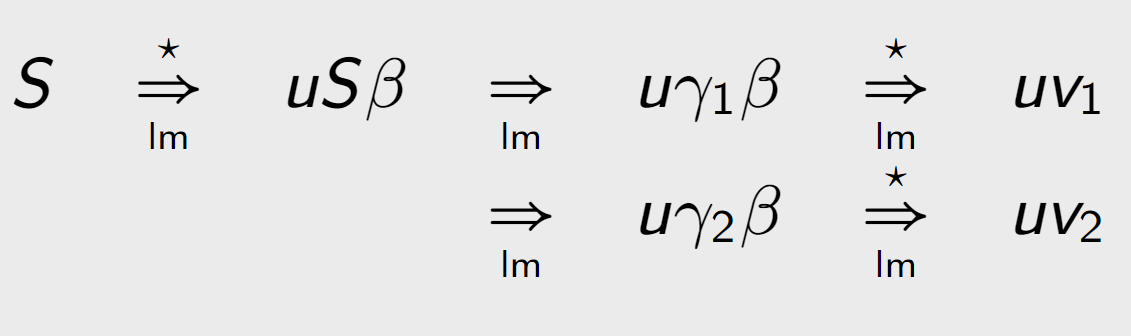
\includegraphics[scale=0.3]{img/cap5/ejemplo13_1.png}
    \end{figure}
    % \img{img/cap5/ejemplo13.png}{0.3}
    Como $v_1|_1 = v_2|_1 = n$ pero $\gamma_1 \neq \gamma_2$, entonces $\ca{G}_3$ NO es una gramática $\gll(1)$.
    % \img{img/cap5/ejemplo13_1.png}{0.3}
    \begin{itemize}
        \item Si $v_1|_2 = v_2|_2 = n+$, entonces $\gamma_1 = \gamma_2 = n + S$.
        \item Si $v_1|_1 = v_2|_1 = na$, con $a \neq +$, entonces $\gamma_1 = \gamma_2 = n$.
    \end{itemize}
    Por lo tanto, tenemos que $\gamma_1 = \gamma_2$ y entonces $\ca{G}_3$ es $\gll(2)$.
}
\ejemplo{Gramática NO $\gll(k)$}{}{
\img{img/cap5/ejemplo14.png}{0.35}
Como $v_1|_k = v_2|_k = (\overset{k}{\cdots}($ pero $\gamma_1 \neq \gamma_2$, entonces $\ca{G}_4$ NO es una gramática $\gll(k)$ para todo $k$.
    }

    \ejemplo{Gramática NO $\gll(k)$ transformada en $\gll(2)$}{}{
        La gramática $\ca{G}_4$ del ejemplo anterior se puede transformar para que sea $\gll(2)$ de la siguiente manera:
        \img{img/cap5/ejemplo15.png}{0.35}

        Queda como ejecicio para el lector demostrar que $\ca{G}_4'$ es $\gll(2)$.
    }

    \ejemplo{Lenguaje NO $\gll(k)$}{}{
        \img{img/cap5/ejemplo16.png}{0.35}
        Para todo $k\ge 1$, se tiene que $\ca{G}_5$ NO es una gramática $\gll(k)$. \medbreak

        Es posible demostrar que, para toda gramática $\ca{G}$ con $\ca{L}(\ca{G}_5) = \ca{L}(\ca{G})$, $\ca{G}$ NO es una gramática $\gll(k)$ para todo $k \geq 1$.
    }

    \subsubsection{Caracterización LL}
    Para esta parte es importante manejar las definiciones de prefijos vistas en la sección \ref{prefijos}. \medbreak

    Sea $\ca{G} = (V,\Sigma,P,S)$ una gramática libre de contexto \textbf{reducida} y $k \ge 1$. En base a esto definimos el siguiente teorema:

    \teorema{}{}{
        $\ca{G}$ es una gramática $\gll(k)$ si, y sólo si, para todas dos reglas distintas $Y\to\gamma_1,Y\to\gamma_2 \in P$ y para todo $S\ \overunder{\Rightarrow}{\mathrm{lm}}{*}\ uY\beta$, se tiene que:
        $$
            \first_k(\gamma_1 \beta)\ \cap\ \first_k(\gamma_2 \beta) = \varnothing
        $$

    }

    \paragraph{Demostración.} $(\Rightarrow)$ Por contrapositivo, supongamos que $v\in \first_k(\gamma_1 \beta) \cap \first_k(\gamma_2 \beta)$. Como $\ca{G}$ es reducida (sin variables inútiles), entonces
    \begin{align*}
        S \quad \overunder{\Rightarrow}{\mathrm{lm}}{*} \quad u Y \beta \quad & \overunder{\Rightarrow}{\mathrm{lm}}{}\ u \gamma_1 \beta \ \overunder{\Rightarrow}{\mathrm{lm}}{*} u v v_1 \\
                                                                              & \overunder{\Rightarrow}{\mathrm{lm}}{}\ u \gamma_2 \beta \ \overunder{\Rightarrow}{\mathrm{lm}}{*} u v v_2
    \end{align*}
    para algún $v_1,v_2 \in \Sigma^*$. Como $\gamma_1 \neq \gamma_2$, entonces $\ca{G}$ NO es $\gll(k)$. \medbreak

$(\Leftarrow)$ Por contrapositivo (de nuevo), supongamos que $\ca{G}$ no es $\gll(k)$. Como $\ca{G}$ no es $\gll(k)$, entonces tenemos derivaciones de la forma:
    \begin{align*}
        S \quad \overunder{\Rightarrow}{\mathrm{lm}}{*} \quad u Y \beta \quad & \overunder{\Rightarrow}{\mathrm{lm}}{}\ u \gamma_1 \beta \ \overunder{\Rightarrow}{\mathrm{lm}}{*} u v_1 \\
                                                                              & \overunder{\Rightarrow}{\mathrm{lm}}{}\ u \gamma_2 \beta \ \overunder{\Rightarrow}{\mathrm{lm}}{*} u v_2
    \end{align*}
    Vemos que $v_1|_k = v_2|_k = v$, pero $\gamma_1 \neq \gamma_2$. Por lo tanto, $v \in \first_k(\gamma_1 \beta) \cap \first_k(\gamma_2 \beta)$. \hfill $\blacksquare$ \bigbreak

    ¿Cómo usamos la caracterización del teorema para demostrar que una gramática es $\gll(k)$? Buscaremos condiciones más simples para verificar si una gramática es $\gll(k)$.

    \paragraph{Definición.} $\ca{G}$ es una gramática $\gll(k)$ \textbf{fuerte} si para todas dos reglas distintas $Y \to \gamma_1, Y\to \gamma_2 \in P$ se tiene que:
    \alignformula{
        \first_k(\gamma_1) \odot_k \follow_k(Y)\ \cap\ \first_k(\gamma_2) \odot_k \follow_k(Y) = \varnothing
    }

    \ejemplo{Si $\ca{G}$ es $\gll(k)$ fuerte, entonces $\ca{G}$ es $\gll(k)$}{}{
        Una gramática $\ca{G}$ que sea $\gll(k)$ fuerte siempre es $\gll(k)$, ya que si definimos dos conjuntos dados por el teorema de $\gll(k)$ $(F_1)$ y la definición de $\gll(k)$ fuerte $(F_2)$, dados por:
        \begin{align*}
            F_1 & = \first_k(\gamma_1 \beta)\ \cap \ \first_k(\gamma_2 \beta) = \first_k(\gamma_1) \odot_k \first_k(\beta) \ \cap \ \first_k(\gamma_2) \odot_k \first_k(\beta) \\
            F_2 & = \first_k(\gamma_1) \odot_k \first_k(Y) \ \cap \ \first_k(\gamma_2) \odot_k \first_k(Y) = \varnothing
        \end{align*}
        Entonces, tenemos que $F_1 \subseteq F_2$.
    }

    \ejemplo{Si $\ca{G}$ es $\gll(k)$, ¿es $\gll(k)$ fuerte?}{}{
        La respuesta directa es que no. Con un contrajemplo, tomemos la gramática $\ca{G}$ definida por
        \begin{align*}
            \ca{G}: \quad S & \to aXaa \mid bXba  \\
            X               & \to b \mid \epsilon
        \end{align*}
        \textbf{Recordatorio:} $\ca{G}$ es $\gll(k)$ si para todas dos reglas distintas $Y\to\gamma_1,Y\to\gamma_2 \in P$ y para todo $S \ \overunder{\Rightarrow}{\mathrm{lm}}{*}\ uY \beta$, se tiene que
        $$
            \first_k(\gamma_1 \beta) \ \cap \ \first_k(\gamma_2 \beta) = \varnothing
        $$
        \begin{itemize}
            \item Si $S \ \overunder{\Rightarrow}{\mathrm{lm}}{*}\ aXaa$, entonces $\first_2(baa) \ \cap \ \first_2(aa) = \varnothing$.
            \item Si $S \ \overunder{\Rightarrow}{\mathrm{lm}}{*}\ bXba$, entonces $\first_2(baa) \ \cap \ \first_2(ba) = \varnothing$
        \end{itemize}
        Por lo tanto, $\ca{G}$ es $\gll(2)$. \medbreak

        \textbf{Recordatorio:} $\ca{G}$ es una gramática $\gll(k)$ fuerte si para todas dos reglas distintas $Y\to\gamma_1,Y\to\gamma_2 \in P$ se tiene que:
        $$
            \first_k(\gamma_1) \odot_k \follow_k(Y)\ \cap\ \first_k(\gamma_2) \odot_k \follow_k(Y) = \varnothing
        $$
        Si vemos $X\to b$ y $X\to \epsilon$:
        \begin{align*}
            \first_2(b) & \odot_2 \follow_2(X)\ \cap\ \first_2(\epsilon) \odot_2 \follow_2(X)       \\
                        & = \{b\} \odot_2 \{aa, ba\} \ \cap \ \{\epsilon\} \odot_2 \{aa, ba\}       \\
                        & = \{ba, bb\} \ \cap \ \{aa, ba\}                                          \\
                        & = \{ba\} \qquad \qquad \text{y por ende $\ca{G}$ no es $\gll(2)$ fuerte.}
        \end{align*}
    }

    ¿Qué pasa con el caso $\gll(1)$? Supongamos que $\ca{G}$ es $\gll(1)$ y $Y\to\gamma_1, Y\to\gamma_2 \in P$ son reglas distintas.
    \begin{enumerate}
        \item Si $\epsilon \notin \first_1(\gamma_1)$ y $\epsilon \not\in \first_1(\gamma_2)$, entonces, por la caracterización de $\gll(1)$:
              \begin{align*}
                  \varnothing & = \first_1(\gamma_1 \beta) \ \cap \ \first_1(\gamma_2 \beta)                               \\
                              & = \first_1(\gamma_1) \ \cap \ \first_1(\gamma_2)                                           \\
                              & = \first_1(\gamma_1) \odot_1 \follow_1(Y) \ \cap \ \first_1(\gamma_2) \odot_1 \follow_1(Y)
              \end{align*}
        \item Si $\epsilon \in \first_1(\gamma_1)$ y $\epsilon \notin \first_1(\gamma_2)$, entonces, por la caracterización de $\gll(1)$:
              \begin{align*}
                  \varnothing & = \first_1(\gamma_1 \beta) \ \cap \ \first_1(\gamma_2 \beta)  \\
                              & = \first_1(\gamma_1 \beta) \ \cap \ \first_1(\gamma_2)        \\
                              & = \first_1(\gamma_1 \beta) \ \cap \ \first_1(\gamma_2 \beta') \\
              \end{align*}
              para todo $\beta' \in (V \cup \Sigma)^*$. Por lo tanto:
              \begin{align*}
                   & \first_1(\gamma_1) \odot_1 \follow_1(Y) \ \cap \ \first_1(\gamma_2) \odot_1 \follow_1(Y)                                                                                                            \\
                   & = \bigcup_{S \overunder{\Rightarrow}{\mathrm{lm}}{*}uY\beta} \first_1(\gamma_1 \beta) \ \cap \ \bigcup_{S \overunder{\Rightarrow}{\mathrm{lm}}{*}uY\beta'} \first_1 (\gamma_2 \beta') = \varnothing
              \end{align*}
    \end{enumerate}

    Por lo tanto, establecemos el siguiente teorema.

    \teorema{}{}{
        Una gramática $\ca{G}$ es $\gll(1)$ si, y sólo si, $\ca{G}$ es $\gll(1)$ \textbf{fuerte}, esto es, para todas dos reglas distintas $Y \to \gamma_1, Y \to \gamma_2 \in P$:
        $$
            \first_1(\gamma_1) \odot_1 \follow_1(Y)\ \cap\ \first_1(\gamma_2) \odot_1 \follow_1(Y) = \varnothing
        $$
    }
    La condición del teorema anterior se puede verificar en \textbf{tiempo polinomial} en $\ca{G}$.

    \subsection[Parsing con gramáticas LL(k)]{Parsing con gramáticas $\gll(k)$}
    \subsubsection{Algunas consideraciones}
    Considere la siguiente gramática $\ca{G}$:
    \begin{align*}
        S & \to Xa \mid Xb \\
        X & \to c
    \end{align*}

    ¿Es esta gramática del tipo $\gll(1)$? Podemos ver que $\first_1(\gamma_1 \beta) = \{c\}$ y $\first_1(\gamma_2 \beta) = \{c\}$, con $\gamma_1 = Xa$, $\gamma_2 = Xb$ y $\beta = \epsilon$. Por lo tanto su intersección no es vacía y entonces $\ca{G}$ no es $\gll(1)$. ¿Podemos establecer una solución para este problema?

\paragraph{Factorización.} En general, si tenemos una regla:
$$
    X \to \gamma\alpha_1 \mid \gamma \alpha_2
$$
siempre podemos ``\textbf{factorizar}'' la regla manteniendo la semántica, como:
\begin{align*}
    X  & \to \gamma X'              \\
    X' & \to \alpha_1 \mid \alpha_2
\end{align*}

Considere ahora la siguiente gramática $\ca{G}$:
$$
    E \to E * E \mid n
$$

¿Es esta gramática del tipo $\gll(1)$? ¿$\gll(k)$? Pues no es ninguna. El problema con esta gramática es su recursividad, en específico, por la izquierda.

\paragraph{Definición.} Una gramática $\ca{G}$ se dice \textbf{recursiva por la izquirrda} si existe $X \in V$ tal que:
\alignformula{
    X \overunder{\Rightarrow}{}{+} X\gamma \quad \text{para algún }\gamma \in (V \cup \Sigma)^*
}

\teorema{}{}{
    Si $\ca{G}=(V,\Sigma,P,S)$ es una gramática reducida y recursiva por la izquierda, entonces $\ca{G}$ NO es $\gll(k)$ para todo $k \ge 1$.
}
\paragraph{Demostración.} Por simplicidad, suponga que $X \to X\beta \in P$ y $X \to w \in P$. \medbreak

Como $\ca{G}$ es reducida, entonces existe una derivación $S \overunder{\Rightarrow}{\mathrm{lm}}{*} uX\gamma$:
$$
    S \ \overunder{\Rightarrow}{\mathrm{lm}}{*} \ uX\gamma \ \overunder{\Rightarrow}{\mathrm{lm}}{} \ \overset{n\text{-veces}}{\cdots}\ \overunder{\Rightarrow}{\mathrm{lm}}{} \ uX \beta^n\gamma
$$
Por \textbf{contradicción}, suponga que $\ca{G}$ es $\gll(k)$. Por lo tanto:
$$
    \first_k(X\beta^{n+1}\gamma) \ \cap \ \first_k(w \beta^n \gamma) = \varnothing
$$
Suponga que $\beta \overunder{\Rightarrow}{}{*} v \in \Sigma^*$ y $\gamma \overunder{\Rightarrow}{}{*} v' \in \Sigma^*$. Con $n = k$, tendremos que
$$
    (wv^k v')|_k \quad \in \quad \first_k(X\beta^{k+1}\gamma) \ \cap \ \first_k(w \beta^k\gamma) \quad \rightarrow\leftarrow \text{ (¡contradicción! el conjunto no es vacío)}
$$
\hfill $\blacksquare$ \bigbreak

Hablemos de recursión \textbf{inmediata} por la izquierda. Suponga que existe $X \in V$ tal que:
$$
    X \to X \alpha_1 \mid \cdots \mid X \alpha_m \mid \beta_1 \mid \cdots \mid \beta_n
$$
¿Cómo podemos \textbf{eliminar} la recursión inmediata por la izquierda? Consideramos la misma gramática pero \textbf{cambiando} las reglas de $X$ por:
\begin{align*}
    X  & \to \beta_1 X' \mid \cdots \mid \beta_n X'                 \\
    X' & \to \alpha_1 X' \mid \cdots \mid \alpha_m X' \mid \epsilon
\end{align*}
\ejemplo{Eliminando recursión inmediata}{}{
    \img{img/cap5/ejemplo19.png}{0.4}
}

\teorema{}{}{
    Sea $\ca{G}$ una gramática tal que existe $X \in V$:
    $$
        X \to X \alpha_1 \mid \cdots \mid X \alpha_m \mid \beta_1 \mid \cdots \mid \beta_n
    $$
    Sea $\ca{G}'$ la misma gramática $\ca{G}$ pero cambiando las reglas de $X$ por:
    \begin{align*}
        X  & \to \beta_1 X' \mid \cdots \mid \beta_n X'                 \\
        X' & \to \alpha_1 X' \mid \cdots \mid \alpha_m X' \mid \epsilon
    \end{align*}
    Entonces $\ca{L}(\ca{G})=\ca{L}(\ca{G}')$
}

\paragraph{Demostración.} Una derivación por la izquierda de $X$ en $\ca{G}$:
$$
    X \ \underset{\mathrm{lm}}{\Rightarrow} \ X \alpha_{i_1} \ \underset{\mathrm{lm}}{\Rightarrow} \ X \alpha_{i_2} \alpha_{i_1} \ \underset{\mathrm{lm}}{\Rightarrow} \ \cdots \ \underset{\mathrm{lm}}{\Rightarrow}\ X \alpha_{i_p} \alpha_{i_{p-1}} \cdots \alpha_{i_1} \ \underset{\mathrm{lm}}{\Rightarrow} \ \beta_j \alpha_{i_p} \alpha_{i_{p-1}} \cdots \alpha_{i_1}
$$
Una derivación por la derecha de $X$ en $\ca{G}'$ \textbf{equivalente}:
$$
    X \ \underset{\mathrm{rm}}{\Rightarrow} \ \beta_j X' \ \underset{\mathrm{rm}}{\Rightarrow} \ \beta_j \alpha_{i_p} X' \ \underset{\mathrm{rm}}{\Rightarrow} \ \cdots \ \underset{\mathrm{rm}}{\Rightarrow}\ \beta_j \alpha_{i_p} \cdots \alpha_{i_2} \alpha_{i_1} X' \ \underset{\mathrm{rm}}{\Rightarrow} \ \beta_j \alpha_{i_p} \alpha_{i_{p-1}} \cdots \alpha_{i_1}
$$
\hfill $\blacksquare$ \bigbreak

Ahora, ¿qué pasa si la recursión por la izquierda es \textbf{no-inmediata}? Considere la siguiente gramática \textbf{recursiva por la izquierda}:
\begin{align*}
    S & \to Xa \mid b \\
    X & \to Yc        \\
    Y & \to Xd \mid e
\end{align*}

¿Cómo eliminamos la recursión por la izquierda no-inmediata?
\paragraph{Estrategia.} Dado $V = \{X_1,\ldots,X_n\}$, removemos la recursión inductivamente en $n$, tal que, en cada paso $i$ de la inducción, se cumplira que para todo $i,j\leq n$:
$$
    \text{si } X_i \to X_j \alpha, \text{ entonces } i < j
$$

\vspace{-15pt}
\begin{algorithm}[hbt!]
    % \caption*{An algorithm with caption}\label{alg:two}
    \setstretch{1.25}
    \DontPrintSemicolon
    \SetKwFunction{FEliminarRecursion}{EliminarRecursion}
    \SetKwProg{Fn}{Function}{:}{}
    \SetKwInOut{Input}{input}\SetKwInOut{Output}{output}
    \Input{Gramática $\ca{G}=(V,\Sigma,P,S)$ y $V=\{X_1,\ldots,X_n\}$}
    \Output{Gramática $\ca{G}$ sin recursión por la izquierda}
    \Fn{\FEliminarRecursion{$\ca{G}$}}{
        $P':=P$

        \For{$i=1$ \KwTo $n$}{
            \For{$j=1$ \KwTo $i-1$}{
                \ForEach{$X_i \to X_j \gamma \in P'$}{
                    \ForEach{$X_j \to \alpha \in P'$}{
                        $P' := P' \cup \{X_i \to \alpha\gamma\}$
                    }
                    $P' := P' - \{X_i \to X_j \gamma\}$
                }
            }
            Remover recursión inmediata para $X_i$ en $P'$ (si existe)
        }
        $V' := \{X_1,\ldots,X_n\} \cup \{X_1',\ldots,X_n'\}$

        \Return{$(V',\Sigma,P',S)$}
    }
\end{algorithm}

Queda como ejercicio propuesto al lector demostrar la correctitud del algoritmo.

\ejemplo{Eliminando recursión}{}{
    \begin{align*}
        E & \to E + T \mid T \\
        T & \to T * F \mid F \\
        F & \to (E) \mid n
    \end{align*}
    Eliminando la \textbf{recursión inmediata} de $E$:
    \begin{align*}
        E  & \to TE'                \\
        E' & \to +TE' \mid \epsilon \\
        T  & \to T * F \mid F       \\
        F  & \to (E) \mid n
    \end{align*}
    Eliminando la \textbf{recusión inmediata} de $T$:
    \begin{align*}
        E  & \to TE'                \\
        E' & \to +TE' \mid \epsilon \\
        T  & \to FT'                \\
        T' & \to *FT' \mid \epsilon \\
        F  & \to (E) \mid n
    \end{align*}
}
\vspace{-10pt}
\paragraph{Conclusión.} Es \textbf{posible eliminar} la recursividad por la izquierda, pero esto \textbf{NO asegura} que el resultado sea una gramática $\gll(k)$ para algún $k$.

\subsubsection[Parsing de LL(k)]{Parsing de $\gll(k)$}
\fig{img/cap5/parsing_llk.png}{0.4}{Máquina de parsing}

\paragraph{Definición.} Sea $\Sigma$ un alfabeto finito. Se definen los siguientes conjuntos de palabras:
\begin{itemize}
    \item $\dot{\Sigma}= \Sigma^* \times \Sigma^*$
    \item $\dot{\Sigma}^{\le k} = \{ (u,v) \in \dot{\Sigma} \mid |uv| \le k \}$
    \item $\dot{\Sigma}_{\#}^{\le k} = \{ (u,v) \in \dot{\Sigma} \mid |uv| \le k \} \cup \{ (u,v\#) \mid (u,v) \in \dot{\Sigma} \mid |uv| < k \}$
\end{itemize}

\paragraph{Notación.} En vez de usar $(u,v) \in \dot{\Sigma}_{\#}^{\le k}$, escribiremos $u.v \in \dot{\Sigma}_{\#}^{\le k}$. El par $\epsilon.\epsilon$ lo denotaremos solamente por $\epsilon$.

\paragraph{Definición.} Un transductor apilador con $k$-lookahead ($k$-PDT) es una tupla:
\alignformula{
    \ca{T} = (Q, \Sigma, \Omega, \Delta, q_0, F)
}

\begin{itemize}
    \item $Q$ es un conjunto finito de estados.
    \item $\Sigma$ es el alfabeto de input.
    \item $\Omega$ es el alfabeto de output.
    \item $\Delta \subseteq Q^{+} \times \dot{\Sigma}_{\#}^{\leq k} \times(\Omega \cup\{\epsilon\}) \times Q^*$ es la relación de transición.
    \item $q_0 \in Q$ es un conjunto de estados iniciales.
    \item $F \subseteq Q$ es el conjunto de estados finales.
\end{itemize}

\paragraph{Definición.} Una \textbf{configuración} de $\ca{T}$ es una tupla:
\alignformula{
    \left(q_1 \ldots q_k, w, o\right) \in\left(Q^{+}, \Sigma^* \cdot\{\#\}, \Omega^*\right)
}
\begin{itemize}
    \item $q_1\ldots q_k$ es el contenido del stack con $q_1$ el tope del stack.
    \item $w$ es el contenido del input.
    \item $o$ es el contenido del output.
\end{itemize}
Decimos que una configuración:
\begin{itemize}
    \item $(q_0, w\#, \epsilon)$ es \textbf{inicial} y
    \item $(q_f, \#, o)$ es \textbf{final} si $q_f \in F$.
\end{itemize}

\paragraph{Definición.} Se define la relación $\vdash_{\ca{T}}$ de \textbf{siguiente-paso} entre configuraciones de $\ca{T}$:
\alignformula{
    \left(\gamma_1, w_1, o_1\right)\ \vdash_\mathcal{T}\ \left(\gamma_2, w_2, o_2\right)
}
si, y sólo si, existe $(\alpha,u.v,a,\beta) \in \Delta$, $\gamma \in \Gamma^*$ y $w \in \Sigma^* \cdot \{\#\}$ tal que:
\begin{itemize}
    \item \textbf{Stack:} $\gamma_1 = \alpha \cdot \gamma$ y $\gamma_2 = \beta \cdot \gamma$
    \item \textbf{Look-ahead:} $w_1 = u \cdot v \cdot w$ y $w_2 = v \cdot w$
    \item \textbf{Output:} $o_2 = o_1 \cdot a$
\end{itemize}
Se define $\vdash_{\ca{T}}^*$ como la clausura \textbf{refleja} y \textbf{transitiva} de $\vdash_{\ca{T}}$.

\paragraph{Definición.} $\ca{T}$ \textbf{entrega} $o$ con \textbf{input} $w$ si existe una configuración inicial $(q_0, w\cdot \#, \epsilon)$ y una configuración final $(q_f, \#, o)$ tal que:
$$
    \left(q_0, w \cdot \#, \epsilon\right) \vdash_{\mathcal{T}}^*\left(q_f, \#, o\right)
$$
Se define la función $\llbracket \ca{T} \rrbracket: \Sigma^* \to 2^{\Omega^*}$:
\alignformula{
    \llbracket \mathcal{T} \rrbracket(w)=\left\{o \in \Omega^* \mid \mathcal{T} \text { entrega } o \text { con input } w\right\}
}

\paragraph{Definición.} $\ca{T}$ es \textbf{determinista} si para todo $\left(\alpha_1, u_1.v_1, a_1, \beta_1\right),\left(\alpha_2, u_2.v_2, a_2, \beta_2\right) \in \Delta$ con \\
$\left(\alpha_1, u_1.v_1, a_1, \beta_1\right) \neq\left(\alpha_2, u_2.v_2, a_2, \beta_2\right)$ se cumple que
\alignformula{
    \alpha_1 \text { NO es prefijo de } \alpha_2 \quad \text{o} \quad u_1 v_1 \text { NO es prefijo de } u_2 v_2 \text {. }
}
\textit{``Para cualquier configuración $(\gamma, w, o)$ existe \textbf{a lo más} una configuración $(\gamma', w', o)$ tal que $(\gamma,w,o) \vdash_{\ca{T}}^* (\gamma',w', o')$''} \medbreak

La \textbf{ventaja} de un $k$-PDT determinista es que nos aseguramos de que siempre obtenemos un solo output para cada input (el no-determinismo nos podría generar muchos outputs distintos).

\paragraph{Construcción del parser.} Sea $\ca{G}=(V,\Sigma, P, S)$ una gramática $\gll(k)$ fuerte. Se define el $k$-PDT para $\ca{G}$:
\alignformula{
    \ca{T}[\ca{G}]= \Big( V\cup \Sigma \cup \{q_0,q_f\},\Sigma, \underbrace{P}_\Omega, \Delta, q_0, \{q_f\} \Big)
}
La relación de transición $\Delta$ de define como:
\begin{table}[H]
    \centering
    \begin{tabular}{rl}
        \textbf{Inicio:}   & $(q_0, \epsilon., \epsilon, S\cdot q_f)$                                                \\
        \textbf{Reducir:}  & $(a, a., \epsilon, \epsilon)$ para cada $a \in \Sigma$                                  \\
        \textbf{Expandir:} & $(X, .u, p, \gamma)$                                                                    \\
                           & para cada $p:=(X\to\gamma) \in P$ tal que $u \in \first_k(\gamma) \odot_k \follow_k(X)$
    \end{tabular}
\end{table}

\paragraph{Propiedades.} $\ca{T}[\ca{G}]$ tiene las siguientes propiedades:
\begin{enumerate}
    \item $\ca{T}[\ca{G}]$ es un $k$-PDT \textbf{determinista} si, y sólo si, $\ca{G}$ es $\gll(k)$ fuerte.
    \item Si $w \notin \ca{L}(\ca{G})$ entonces $\llbracket \ca{T} \rrbracket (w) = \varnothing$.
    \item Si $w \in \ca{L}(\ca{G})$ entonces $\llbracket \ca{T} \rrbracket(w) = \{r_1 \ldots r_m\}$ es una derivación por la izquierda de $\ca{G}$ sobre $w$.
\end{enumerate}

\paragraph{Algoritmo.} Para una gramática $\gll(k)$ $\ca{G}$ y una palabra $w \in \Sigma^*$:
\begin{enumerate}
    \item Construya el $k$-PDT determinista $\ca{T}[\ca{G}]$ a partir de $\ca{G}$.
    \item Ejecute $\ca{T}[\ca{G}]$ sobre $w$.
\end{enumerate}

Como $\ca{T}[\ca{G}]$ es determinista, entonces el algoritmo toma \textbf{tiempo lineal} en $w$.

\paragraph{Tabla predictiva para $\gll(k)$ fuerte.} Sea $\ca{G}=(V,\Sigma, P, S)$ una gramática $\gll(k)$ fuerte. Para cada $u \in \Sigma^k \cup \Sigma^{<k}\cdot \{\#\}$, se define $M[X,u] \in (V\cup \Sigma)^* \cup \{\texttt{ERROR}\}$:

\alignformula{
    M[X, u]= \begin{cases}
        \quad\gamma       & \text { si } X \rightarrow \gamma \in P \text { y } u \in \first_k(\gamma) \odot_k \follow_k(X) \\
        \texttt { ERROR } & \text { en otro caso. }
    \end{cases}
}
El computo de la tabla predictiva puede tomar \textbf{tiempo exponencial} en $|\ca{G}|$ y $k$.

\paragraph{Caso especial: tabla predictiva para $\gll(1)$.} Sea $\ca{G}=(V,\Sigma, P, S)$ una gramática $\gll(1)$ fuerte. Para cada $a \in \Sigma \cup \{\#\}$, se define $M[x,a] \in (V \cup \Sigma)^* \cup \{\texttt{ERROR}\}$:
\alignformula{
    M[X, a]= \begin{cases}
        \quad \gamma    & \text { si } X \rightarrow \gamma \in P \text { y } a \in \first_1(\gamma)                            \\
        \quad \gamma    & \text { si } X \rightarrow \gamma \in P, \epsilon \in \first_1(\gamma) \text { y } a \in \follow_1(X) \\
        \text { ERROR } & \text { en otro caso. }
    \end{cases}
}
Este cálculo se puede hacer en tiempo $\ca{O}(|V|\cdot|P|)$.

\ejemplo{Tabla predictiva}{}{
    \img{img/cap5/ejemplo21.png}{0.5}
}

\section{Extracción de información}

\subsection{Extracción}

Imaginemos que tenemos un log de la forma
$$
    \begin{array}{lll}
        \texttt{18:30} & \texttt{ ERROR 06} \\
        \texttt{19:10} & \texttt{ OK 00}    \\
        \texttt{20:00} & \texttt{ ERROR 19}
    \end{array}
$$
y queremos obtener todas las horas $\texttt{HH:MM}$, quizá con una expresión regular $R =$ ({\textbackslash}d{\textbackslash}d:{\textbackslash}d{\textbackslash}d). ¿Cómo podemos \textbf{automatizar} esta tarea de extraer datos?
\begin{enumerate}
    \item Una tarea como la anterior \textbf{se puede programar fácilmente}, ¿por qué queremos automatizarla?
    \item Las expresiones regulares ya hacen el trabajo anterior, ¿por qué queremos \textbf{estudiar este problema de nuevo}?
\end{enumerate}
En esta última sección veremos \textbf{nuevas técnicas formales y algorítmicas} para entender y resolver este problema.

\subsubsection{Spans}

\paragraph{Definición.} Para un documento $d = a_0 a_1 \ldots a_{n-1}$ se define un \textbf{span} $s$ de $d$ como:
\alignformula{
s=[i, j\rangle
}
tal que $0 \leq i \leq j \leq n$. \bigbreak

Si $s = [i,j \rangle$ es un span de $d$ se define:
\alignformula{
d[s]=d[[i, j\rangle]=a_i a_{i+1} \ldots a_{j-1}
}
como el \textbf{contenido del span} $s$ en $d$. Si $i = j$, entonces $d[[i, i\rangle]=\epsilon$.
\ejemplo{}{}{
    \vspace{-10pt}
    \img{img/cap6/ejemplo1.png}{0.4}
}

Denotamos el conjunto de \textbf{todos los spans} de $d$ como $\texttt{Spans}(d)$.

\newpage
\subsubsection{Regex}
\paragraph{Sintaxis.} Sea $\Sigma$ un alfabeto finito y $\ca{X}$ un conjunto de variables. $R$ es una expresión regular con variables (o \textbf{regex}) sobre $\Sigma$ si $R$ es igual a:
\begin{enumerate}
    \item $a$, para alguna letra $a \in \Sigma$.
    \item $\epsilon$
    \item $\mathbf{x}\{R_1\}$, donde $R_1$ es una regex y $\mathbf{x} \in X$.
    \item $(R_1 + R_2)$, donde $R_1$ y $R_2$ son regex.
    \item $(R_1 \cdot R_2)$, donde $R_1$ y $R_2$ son regex.
    \item $(R_1^*)$, donde $R_1$ es una regex.
\end{enumerate}

$\mbb{x}\{R_1\}$ representa que el \textbf{span capturado} por $R_1$ lo almacenaremos en la variable $\mbb{x}$.

\ejemplo{}{}{
    Sea $\Sigma = \{a,b,\sbar\}$.
    \begin{itemize}
        \item $\Sigma^* \cdot \mbb{x}\{abba\} \cdot \Sigma^*$
        \item $\Sigma^* \cdot \sbar \cdot \mbb{x}\{ab \cdot (a+b)^*\}\cdot \sbar \cdot \Sigma^*$
        \item $\Sigma^* \cdot \sbar \cdot \mbb{x}\{(a+b)^*\}\cdot \sbar \cdot \mbb{y}\{(a+b)^*\} \cdot \sbar \cdot \Sigma^*$
        \item $(\Sigma^* \cdot \sbar + \epsilon) \cdot \mbb{z}\{\mbb{x}\{(a+b)^+\}\cdot \sbar \cdot \mbb{y}\{(a+b)^+\}\} \cdot (\epsilon + \sbar \cdot \Sigma^*)$
        \item $\Sigma^* \cdot \mbb{x}\{abba\} \cdot \sbar \cdot \mbb{x}\{baba\} \cdot \Sigma^*$
    \end{itemize}
}

\paragraph{Regex válidas.} Sea $\texttt{Var}(R)$ el conjunto de \textbf{todas las variables} en $\ca{X}$ mencionadas en $R$. Decimos que $R$ es una regex \textbf{válida} si, y sólo si, todas las siguientes condiciones se cumplen:
\begin{enumerate}
    \item si $R = R_1 \cdot R_2$, entonces $\texttt{Var}(R_1) \cap \texttt{Var}(R_2) = \varnothing$, y $R_1$ y $R_2$ son válidas.
    \item si $R = R_1 + R_2$, entonces $\texttt{Var}(R_1) = \texttt{Var}(R_2)$, y $R_1$ y $R_2$ son válidas.
    \item si $R = R_1^*$, entonces $\texttt{Var}(R_1) = \varnothing$, y $R_1$ es válida.
    \item si $R = \mbb{x}\{R_1\}$, entonces $\mbb{x} \notin \texttt{Var}(R_1)$, y $R_1$ es válida.
\end{enumerate}

Si $R$ es \textbf{válida} nos permite asignar las variables de \textbf{manera correcta}.

\ejemplo{}{}{
    Las siguientes regex son válidas:
    \begin{itemize}
        \item $\Sigma^* \cdot \mbb{x}\{abba\} \cdot \Sigma^*$
        \item $\Sigma^* \cdot \mbb{x}\{abba\} \cdot \sbar \cdot \mbb{y}\{baba\} \cdot \Sigma^*$
        \item $\Sigma^* \cdot \sbar \cdot \mbb{x}\{ab\cdot (a+b)^*\} \cdot \sbar \cdot \Sigma^*$
    \end{itemize}
    Las siguientes regex \textbf{no} son válidas:
    \begin{itemize}
        \item $\Sigma^* \cdot \mbb{x}\{abba\} \cdot \sbar \cdot \mbb{x}\{baba\} \cdot \Sigma^*$
        \item $\Sigma^* \cdot (\mbb{x}\{abba\} + \mbb{y}\{baba\}) \cdot \Sigma^*$
        \item $\Sigma^* \cdot \sbar \cdot (\mbb{x}\{ab \cdot (a+b)^*\} \cdot \sbar)^* \cdot \Sigma^*$
    \end{itemize}
}

\paragraph{Mappings.} Un \textbf{mapping} de $R$ sobre un documento $d \in \Sigma^*$ es una función:
\alignformula{
    \mu: \texttt{Var}(R) \to \texttt{Spans}(d)
}

donde el dominio de $\mu$ es $\texttt{dom}(\mu) = \texttt{Var}(R)$. \bigbreak

Se define el mapping $\mu = \, \perp$ como el \textbf{mapping vacío} donde $\texttt{dom}(\perp) = \varnothing$.

\ejemplo{}{}{
    \img{img/cap6/ejemplo4.png}{0.3}
}

\begin{itemize}
    \item Para una variable $\mbb{x}$ y span $s$ se define el \textbf{mapping} de una variable:
          $$
              \mu=[\mathbf{x} \mapsto s] \quad \text { tal que } \quad \texttt{dom}(\mu)=\{\mathbf{x}\} \quad \text { y } \quad \mu(\mathbf{x})=s
          $$

    \item Para $k \in \mathbb{N}$ se define el \textbf{mapping} $\mu + k$ tal que $\texttt{dom}(\mu + k) = \texttt{dom}(\mu)$ y:
          $$
              \text{si } \mu(\mathbf{x})=[i, j\rangle \text { entonces }[\mu+k](\mathbf{x})=[i+k, j+k\rangle \text {.}
          $$

    \item Para mappings $\mu_1,\mu_2$ con $\texttt{dom}(\mu_1) \cap \texttt{dom}(\mu_2) = \varnothing$ se define la \textbf{unión}:
          $$
              \mu=\mu_1 \cup \mu_2 \quad \text { tal que } \quad \mu(\mathbf{x})= \begin{cases}
                  \mu_1(\mathbf{x}) & \text { si } \mathbf{x} \in \operatorname{dom}\left(\mu_1\right) \\
                  \mu_2(\mathbf{x}) & \text { si } \mathbf{x} \in \operatorname{dom}\left(\mu_2\right)
              \end{cases}
          $$
\end{itemize}

\paragraph{Semántica regex.} Para una regex válida $R$ cualquiera, se define la función $\llbracket R \rrbracket$ \textbf{inductivamente} sobre documentos $d \in \Sigma^*$:
\begin{enumerate}
    \item $\llbracket a \rrbracket(d)=\{\perp\}$ si $d = a$, y $\varnothing$ en otro caso.
    \item $\llbracket \epsilon \rrbracket(d)=\{\perp\}$ si $d = \epsilon$, y $\varnothing$ en otro caso.
    \item $\llbracket \mathbf{x}\left\{R_1\right\} \rrbracket(d)=\left\{\mu \cup[\mathbf{x} \mapsto s] \mid \mu \in \llbracket R_1 \rrbracket(d) \text { y } s=[0,|d|\rangle\right\}$
    \item $\llbracket R_1 \cdot R_2 \rrbracket(d)=\left\{\begin{array}{l|l}
                  \mu_1 \cup\left(\mu_2+\left|d_1\right|\right) & \begin{array}{l}
                                                                      \text { existe } d_1, d_2 \text { tal que } d=d_1 \cdot d_2, \\
                                                                      \mu_1 \in \llbracket R_1 \rrbracket\left(d_1\right) \text { y } \mu_2 \in \llbracket R_2 \rrbracket\left(d_2\right)
                                                                  \end{array}
              \end{array}\right\}$

          Como $R_1 \cdot R_2$ son válidas, entonces sabemos que $\texttt{dom}(\mu_1) \cap \texttt{dom}(\mu_2) = \varnothing$.

    \item $\llbracket R_1+R_2 \rrbracket(d)=\llbracket R_1 \rrbracket(d) \cup \llbracket R_2 \rrbracket(d)$

    \item $\llbracket R_1^* \rrbracket(d)=\bigcup_{k=0}^{\infty} \llbracket\left(R_1\right)^k \rrbracket(d)$

          Como $\texttt{Var}(R_1) = \varnothing$, entonces $\llbracket R_1^* \rrbracket(d)=\{\perp\}$ si, y sólo si, $d \in \mathcal{L}\left(R_1^*\right)$.
\end{enumerate}

\ejemplo{}{}{
    \begin{itemize}
        \item $\llbracket b \rrbracket(a) = \varnothing$
        \item $\llbracket b \rrbracket(b) = \{\perp\}$
        \item $\llbracket \mbb{x}\{b\} \rrbracket(a) = \varnothing$
        \item $\llbracket \mbb{x}\{b\} \rrbracket(b) = \{ [\mbb{x} \mapsto [0,1\rangle] \}$
        \item $\llbracket \mathbf{x}\{b\} b \rrbracket(b b)=\{[\mathbf{x} \mapsto[0,1\rangle]\}$
        \item $\llbracket b \mathbf{x}\{b\}\rrbracket(b b)=\{[\mathbf{x} \mapsto[1,2\rangle]\}$
        \item $\llbracket\mathbf{x}\{b\} \mathbf{y}\{b\}\rrbracket(b b)=\{[\mathbf{x} \mapsto[0,1\rangle, \mathbf{y} \mapsto[1,2\rangle]\}$
        \item $\llbracket\mathbf{x}\{b\} b+b \mathbf{x}\{b\}\rrbracket(b b)=\{[\mathbf{x} \mapsto[0,1\rangle],[\mathbf{x} \mapsto[1,2\rangle]\}$
    \end{itemize}
}

\ejemplo{}{}{
    \vspace{-10pt}
    \img{img/cap6/ejemplo6.png}{0.5}

    \begin{itemize}

        \item $\llbracket\Sigma^* \cdot \mathbf{x}\{a b a+b a b\} \cdot \Sigma^*\rrbracket(d)=\{[\mathbf{x} \mapsto[10,13\rangle],[\mathbf{x} \mapsto[11,14\rangle]\}$

        \item $\llbracket\Sigma^* \cdot \sbar \cdot \mathbf{x}\left\{b a \cdot(a+b)^*\right\} \cdot \sbar \cdot \Sigma^*\rrbracket(d)=\{[\mathbf{x} \mapsto[7,9\rangle],[\mathbf{x} \mapsto[10,14\rangle]\}$

        \item $\llbracket\Sigma^* \cdot \mathbf{x}\{a b b a\} \cdot \sbar \cdot \mathbf{y}\{b a\} \cdot \Sigma^*\rrbracket(d)=\{[\mathbf{x} \mapsto[2,6\rangle, \mathbf{y} \mapsto[7,9\rangle]\}$

        \item $\llbracket\Sigma^* \cdot \sbar \cdot \mathbf{x}\left\{(a+b)^*\right\} \cdot \sbar \cdot \mathbf{y}\left\{(a+b)^*\right\} \cdot \sbar \cdot \Sigma^*\rrbracket(d)=\{[\mathbf{x} \mapsto[2,6\rangle, \mathbf{y} \mapsto[7,9\rangle],[\mathbf{x} \mapsto[7,9\rangle, \mathbf{y} \mapsto[10,14\rangle]\}$

        \item $\llbracket\Sigma^* \cdot \mathbf{x}\left\{\Sigma^*\right\} \cdot \Sigma^* \rrbracket(d)=\texttt{Spans}(d)$

    \end{itemize}
}

\paragraph{Evaluación regex.} Podemos preguntarnos:

\begin{itemize}
    \item Dado una regex $R$ con una variable, ¿de qué tamaño puede ser $|\llbracket R \rrbracket(d)|$ con respecto a $|d|$ \textbf{en el peor caso}?
    \item Dado una regex $R$ con $k$ variables, ¿de qué tamaño puede ser $|\llbracket R \rrbracket(d)|$ con respecto a $|d|$ y $k$ \textbf{en el peor caso}?
\end{itemize}

La respuesta es que el tamaño de $|\llbracket R \rrbracket(d)|$ puede crecer de manera exponencial. ¿Cómo podemos evaluar entonces una regex de $R$ \textbf{eficientemente}? Analizamos una herramienta para lograr esto a continuación.

\subsubsection{Vset autómata}

¿Qué tiene de nuevo un autómata con variables (vset autómata)?
\begin{enumerate}
    \item Tiene transiciones con \textbf{abre} y \textbf{cierra} de variable $\mbb{x}$:
          \alignformula{
              p \stackrel{\langle x}{\rightarrow} q \quad y \quad p \stackrel{x\rangle}{\rightarrow} q
          }
    \item Cada ejecución define un \textbf{mapping} de las variables a spans.
\end{enumerate}
Un \textbf{vset autómata} será nuestro primer modelo para \textbf{compilar regex}.

\paragraph{Definición.} Un vset autómata (VA) es una tupla:
\alignformula{
    \ca{A} = (Q, \Sigma, \ca{X}, \Delta, I, F)
}
\begin{itemize}
    \item $Q$ es un conjunto finito de estados.
    \item $\Sigma$ es el alfabeto de input.
    \item $\ca{X}$ es un conjunto finito de variables.
    \item $\Delta \subseteq Q \times(\Sigma \cup\{\epsilon\} \cup\{\langle\mathbf{x}, \mathbf{x}\rangle \mid \mathbf{x} \in \mathcal{X}\}) \times Q$ es la relación de transición.
    \item $I \subseteq Q$ es un conjunto de estados iniciales.
    \item $F \subseteq Q$ es el conjunto de estados finales (o aceptación).
\end{itemize}

`$\langle \mbb{x}$' simboliza \textbf{abrir} y `$\mbb{x}\rangle$' simboliza \textbf{cerrar} la variable $\mbb{x}$.

\ejemplo{vset autómatas}{}{
    \begin{figure}[H]
        \centering
        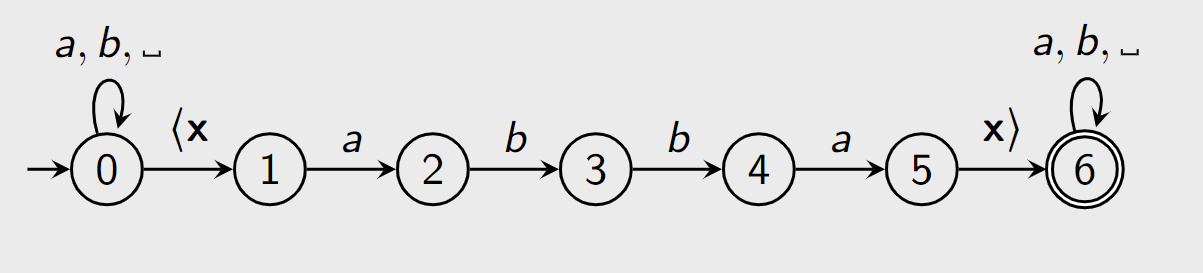
\includegraphics[scale=0.45]{img/cap6/ejemplo7_1.png}
        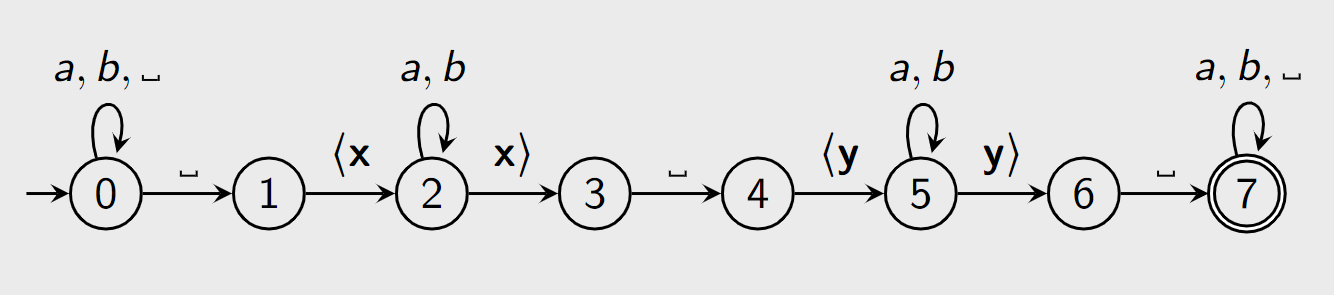
\includegraphics[scale=0.45]{img/cap6/ejemplo7_2.png}
        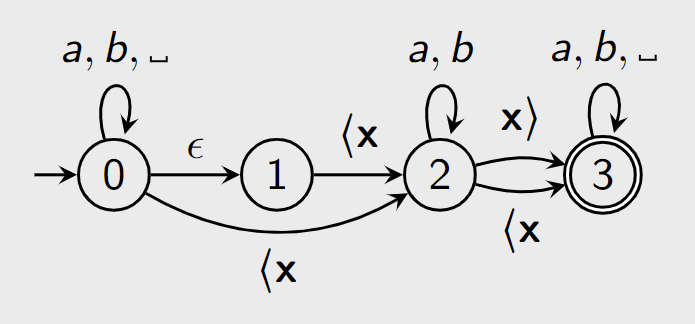
\includegraphics[scale=0.45]{img/cap6/ejemplo7_3.png}
    \end{figure}
}

\paragraph{Ejecución.} Sea $\ca{A} = (Q,\Sigma,\ca{X},\Delta,I,F)$ un VA y $d = a_0 \ldots a_{n-1} \in \Sigma^*$ un documento. Tenemos que:
\begin{itemize}
    \item Un par $(p, i) \in Q \times\{0, \ldots, n\}$ es una \textbf{configuración} de $\ca{A}$ sobre $d$.
    \item Una configuración $(p,0)$ es \textbf{inicial} si $q \in I$.
    \item Una configuración $(p, |d|)$ es \textbf{final} si $q \in F$.
\end{itemize}
\textit{``Intuitivamente, una configuración $(p,i)$ representa que $\ca{A}$ se encuentra en el estado $p$ antes de leer $a_i$''.} \bigbreak

Una \textbf{ejecución} (o \textit{run}) $\rho$ de $\ca{A}$ sobre $d$ es una secuencia:
\alignformula{
    \rho:\left(p_0, i_0\right) \stackrel{o_1}{\rightarrow}\left(p_1, i_1\right) \stackrel{o_2}{\rightarrow} \ldots \stackrel{o_m}{\rightarrow}\left(p_m, i_m\right)
}
tal que cumple todas las siguientes condiciones:
\begin{itemize}
    \item $o_k \in \Sigma \cup\{\epsilon\} \cup\{\langle\mathbf{x}, \mathbf{x}\rangle \mid \mathbf{x} \in \mathcal{X}\}$ con $k \leq m$,
    \item $(p_0, i_0)$ es una configuración inicial,
    \item para todo $k < m$, $\left(p_k, o_{k+1}, p_{k+1}\right) \in \Delta$,
    \item para todo $k \leq m$, si $o_k \in \Sigma$, entonces $o_k = a_{i_{k-1}}$ y $i_k = i_{k-1} + 1$,
    \item para todo $k \leq m$, si $o_k \in\{\epsilon\} \cup\{\langle\mathbf{x}, \mathbf{x}\rangle \mid \mathbf{x} \in \mathcal{X}\}$, entonces $i_k = i_{k-1}$.
\end{itemize}

Una ejecución $\rho$ es de \textbf{aceptación} si $(p_m, i_m)$ es de aceptación.

\ejemplo{Ejecuciones}{}{
    \img{img/cap6/ejemplo8.png}{0.5}
    Algunas ejecuciones sobre $d$:
    \begin{itemize}
        \item $\rho_1:\left(p_0, 0\right) \stackrel{a}{\rightarrow}\left(p_0, 1\right) \stackrel{b}{\rightarrow}\left(p_0, 2\right) \stackrel{a}{\rightarrow}\left(p_0, 3\right)$
        \item $\rho_2:\left(p_0, 0\right) \stackrel{a}{\rightarrow}\left(p_0, 1\right) \stackrel{\epsilon}{\rightarrow}\left(p_1, 1\right) \stackrel{\langle x}{\rightarrow}\left(p_2, 1\right) \stackrel{b}{\rightarrow}\left(p_2, 2\right) \stackrel{\mathrm{x}\rangle}{\rightarrow}\left(p_3, 2\right) \stackrel{a}{\rightarrow}\left(p_3, 3\right)$
        \item $\rho_3:\left(p_0, 0\right) \stackrel{a}{\rightarrow}\left(p_0, 1\right) \stackrel{\langle x}{\rightarrow}\left(p_2, 1\right) \stackrel{b}{\rightarrow}\left(p_2, 2\right) \stackrel{\mathrm{x}\rangle}{\rightarrow}\left(p_3, 2\right) \stackrel{a}{\rightarrow}\left(p_3, 3\right)$
        \item $\rho_4:\left(p_0, 0\right) \stackrel{a}{\rightarrow}\left(p_0, 1\right) \stackrel{\langle x}{\rightarrow}\left(p_2, 1\right) \stackrel{b}{\rightarrow}\left(p_2, 2\right) \stackrel{\langle x}{\rightarrow}\left(p_3, 2\right) \stackrel{a}{\rightarrow}\left(p_3, 3\right)$
    \end{itemize}

    Donde $\rho_2$ y $\rho_3$ son ejecuciones válidas.
}

Una ejecución $\rho$ es \textbf{válida} si, y sólo si, para todo $\mbb{x} \in \ca{X}$:
\begin{itemize}
    \item existe un único $k_1 \leq m$ tal que $o_{k_1} = \mbb{\langle x}$,
    \item existe un único $k_2 \leq m$ tal que $o_{k_2} = \mbb{x\rangle}$ y
    \item $k_1 < k_2$.
\end{itemize}

\textit{``Intuitivamente, $\rho$ es válida si, y sólo si, todas las variables se abren y cierran correctamente.''} \bigbreak

Si $\rho$ es \textbf{válida} se define el \textbf{mapping de} $\rho$ $\texttt{map}(\rho): \ca{X} \to \texttt{Spans}(d)$ tal que:
\alignformula{
[\texttt{map}(\rho)](\mathbf{x})=\left[i_{k_1}, i_{k_2}\right\rangle
}
para todo $\mbb{x} \in \ca{X}$ y $k_1,k_2 \leq m$ con $i_{k_1} = \langle \mbb{x}$ y $i_{k_2} = \mbb{x}\rangle$.

\ejemplo{Mappings de $\rho$}{}{
El mapping para las ejecuciones válidas del ejemplo anterior es:
$$
    \texttt{map}\left(\rho_2\right)=\texttt{map}\left(\rho_3\right)=[\mathbf{x} \mapsto[1,2\rangle]
$$
}

\paragraph{Función de extracción.} Sea $\ca{A}$ un VA. Se define la función $\llbracket \mathcal{A} \rrbracket$ tal que para todo documento $d \in \Sigma^*$:
\alignformula{
    \llbracket \mathcal{A} \rrbracket(d)=\{ \texttt{map}(d) \mid \rho \text{ es una ejecución válida y de aceptación de } \ca{A} \text{ sobre } d\}
}

Un VA nos entrega otra forma de extraer información de un documento.

\subsubsection{Desde regex a VA}

\paragraph{Definición.} Sea $\ca{A}$ un VA. Decimos que $\ca{A}$ es \textbf{funcional} si, y sólo si, para todo documento $d$ y para toda ejecución $\rho$ de $\ca{A}$ sobre $d$:
\alignformula{
    \text{si } \rho \text{ es de aceptación, entonces } \rho \text{ es válida.}
}

Para funcional solo necesitamos verificar que la ejecución es de aceptación.

\teorema{}{}{
Para toda regex $R$ válida, existe un vset autómata \textbf{funcional} $\ca{A}_R$ de \textbf{tamaño lineal} en $|R|$ tal que para todo documento $d$:
$$
    \llbracket R \rrbracket(d)=\llbracket \mathcal{A}_{\mathcal{R}} \rrbracket(d)
$$
}
La demostración de este teorema queda como ejercicio propuesto al lector (es similar al Teorema de Kleene).

\subsection{Enumeración de resultados: Autómatas con anotaciones}

Veamos el siguiente problema:
\begin{table}[H]
    \centering
    \begin{tabular}{ll}
        $\texttt{PROBLEMA:}$ & Evaluación de regex                                         \\
        $\texttt{INPUT:}$    & Una regex $R$ y                                             \\
                             & un documento $w$                                            \\
        $\texttt{OUTPUT:}$   & Enumerar todos los mappings en $\llbracket R \rrbracket(d)$
    \end{tabular}
\end{table}
La idea es:
\begin{enumerate}
    \item Transformamos $R$ a un vset autómata $\ca{A}_R$.
    \item Enumeramos los resultados $\llbracket \mathcal{A}_R \rrbracket(d)$.
\end{enumerate}
¿Cómo computamos todos los mappings en $\llbracket \mathcal{A}_R \rrbracket(d)$? ¿Cómo los encontramos si son demasiados? Veamos qué podemos hacer.

\subsubsection{Representación de mappings}
Sea $d = a_0 \ldots a_{n-1}$, un conjunto de variables $\ca{X}$ y un mapping $\mu: \ca{X} \to \texttt{Spans}(d)$.

\paragraph{Definiciones.} Tenemos que:
\begin{enumerate}
    \item Se define el \textbf{conjunto de marcas de} $\ca{X}$ como:
          \alignformula{
              \texttt{Markers}(\mathcal{X})=\{\langle\mathbf{x}\mid \mathbf{x} \in \mathcal{X}\} \cup\{\mathbf{x}\rangle \mid \mathbf{x} \in \mathcal{X}\}
          }
    \item Se define el \textbf{mapping inverso} de $\mu$ como $\mu^{\text {inv }}:[0, n] \rightarrow 2^{\operatorname{Markers}(\mathcal{X})}$:
          \alignformula{
          \left.\mu^{\text {inv }}(i)=\{\langle\mathbf{x} \mid\exists j.\ \mu(\mathbf{x})=[i, j\rangle \in \mathcal{X}\} \cup\{\mathbf{x}\rangle \mid \exists j.\ \mu(\mathbf{x})=[j, i\rangle \in \mathcal{X}\right\}
          }
    \item Se define la \textbf{secuenciación} de $\mu$ como $\texttt{seq}(\mu) = \texttt{seq}_0(\mu) \cdot \ldots \cdot \texttt{seq}_n(\mu)$:
          \alignformula{
              \texttt{seq}_i(\mu)= \begin{cases}\left(i, \mu^{\mathrm{inv}}(i)\right) & \mu^{\mathrm{inv}}(i) \neq \varnothing \\ \epsilon & \mu^{\mathrm{inv}}(i)=\varnothing\end{cases}
          }

          $\texttt{seq}(\mu)$ es una \textbf{representación equivalente} de un mapping $\mu$, y nos será más conveniente para nuestros algoritmos de enumeración de resultados.
\end{enumerate}

\ejemplo{}{}{
    \vspace{-10pt}
    \img{img/cap6/ejemplo10.png}{0.425}
    $$
        \texttt{seq}(\mu)=(15,\{\langle\mathbf{x},\langle\mathbf{z}\})\ (20,\{\mathbf{x}\rangle\})\ (24,\{\langle\mathbf{y}\})\ (26,\{\mathbf{y}\rangle, \mathbf{z}\rangle\})
    $$
}

\subsubsection{Autómatas con anotaciones}
\paragraph{Definición.} Un autómata con anotaciones (AnnA) es una tupla:
\alignformula{
    \ca{N}=(Q, \Sigma, \Lambda, \Delta, I, F)
}
\begin{itemize}
    \item $Q$ es un conjunto finito de estados.
    \item $\Sigma$ es el alfabeto de input.
    \item $\Lambda$ es un conjunto finito de etiquetas (Labels).
    \item $\Delta \subseteq Q \times(\Sigma \cup \Sigma \times \Lambda) \times Q$ es la relación de transición.
    \item $I \subseteq Q$ es un conjunto de estados iniciales.
    \item $F \subseteq F$ es el conjunto de estados finales (o aceptación).
\end{itemize}

Las transiciones $(p,a,l,q)$ simbolizan que al leer la letra $a$, esta letra \textbf{será anotada} con $l$.
\ejemplo{}{}{
    \begin{figure}[H]
        \centering
        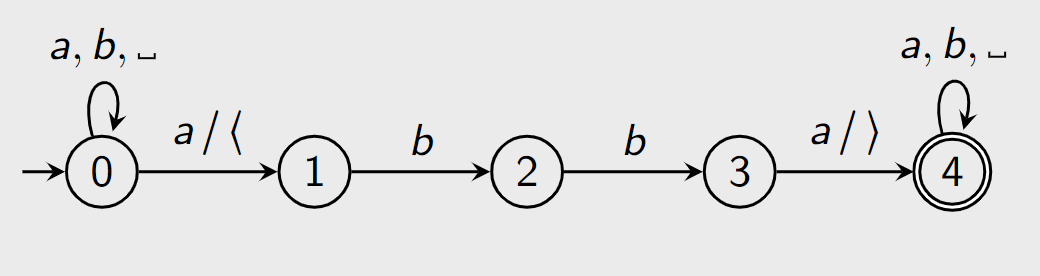
\includegraphics[scale=0.5]{img/cap6/ejemplo11_1.png}
        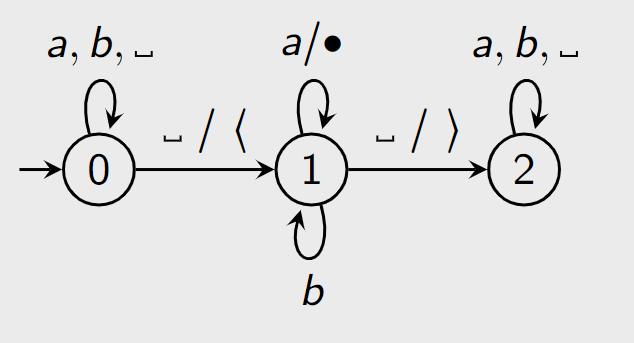
\includegraphics[scale=0.5]{img/cap6/ejemplo11_2.png}
    \end{figure}
}

\paragraph{Ejecución.} Sea un AnnA $\ca{N} = (Q, \Sigma, \Lambda, \Delta, I, F)$ y un documento $d = a_0 \ldots a_{n-1} \in \Sigma^*$. Una \textbf{ejecución} $\rho$ de $\ca{N}$ sobre $d$ es una secuencia:
$$
    \rho: p_0 \stackrel{t_0}{\rightarrow} p_1 \stackrel{t_1}{\rightarrow} \ldots \stackrel{t_{n-1}}{\rightarrow} p_n
$$
tal que cumple todas las siguientes condiciones:
\begin{enumerate}
    \item $p_0 \in I$
    \item para todo $i < n$, $t_i$ es de la forma $t_i = a_i$ o $t_i = (a_i, l)$ para algún $l \in \Lambda$
    \item para todo $i < n$, $(p_i, t_i, p_{i+1}) \in \Delta$
\end{enumerate}

Se define la \textbf{anotación de} $\rho$ como $\texttt{ann}(\rho) = \texttt{ann}_0(t_0) \cdot \ldots \cdot \texttt{ann}_n(t_{n-1})$:
$$
    \texttt{ann}_i(t)= \begin{cases}(i, l) & t=(a, l) \\ \epsilon & t=a\end{cases}
$$
Decimos que $\rho$ es de \textbf{aceptación} si, y sólo si, $q_n \in F$.

\ejemplo{Ejecuciones}{}{
    \vspace{-10pt}
    \img{img/cap6/ejemplo12.png}{0.55}

    Algunas ejecuciones sobre $d$:
    \begin{itemize}

        \item $\rho_1: p_0 \stackrel{a}{\rightarrow} p_0 \stackrel{\sbar / \langle}{\rightarrow} p_1 \stackrel{a / \bullet}{\rightarrow} p_1 \stackrel{b}{\rightarrow} p_1 \stackrel{b}{\rightarrow} p_1 \stackrel{a / \bullet }{\rightarrow} p_1 \stackrel{\sbar / \rangle}{\rightarrow} p_2 \stackrel{b}{\rightarrow} p_2 \stackrel{a}{\rightarrow} p_2 \stackrel{\hphantom{a}\sbar\hphantom{a}}{\rightarrow} p_2 \stackrel{b}{\rightarrow} p_2$

        \item $\rho_2: p_0 \stackrel{a}{\rightarrow} p_0 \stackrel{\hphantom{a}\sbar\hphantom{a}}{\rightarrow} p_0 \stackrel{a}{\rightarrow} p_0 \stackrel{b}{\rightarrow} p_0 \stackrel{b}{\rightarrow} p_0 \stackrel{a}{\rightarrow} p_0 \stackrel{\sbar / \langle}{\rightarrow} p_1 \stackrel{b}{\rightarrow} p_1 \stackrel{a / \bullet}{\rightarrow} p_1 \stackrel{\sbar / \rangle}{\rightarrow} p_2 \stackrel{b}{\rightarrow} p_2$
    \end{itemize}
    Además, tenemos que:
    \begin{itemize}
        \item $\texttt{ann}\left(\rho_1\right)=(1,\langle)(2, \bullet)(5, \bullet)(6,\rangle) \qquad \qquad a \, \overset{\langle}{\sbar} \, \overset{\bullet}{a}\, b\, b\, \overset{\bullet}{a}\, \overset{\rangle}{\sbar}\, b\, a\, \sbar \, b$

        \item $\texttt{ann}\left(\rho_2\right)=(6,\langle)(8, \bullet)(9,\rangle) \qquad \qquad \qquad a \, \sbar \, a \, b \, b \, a \, \overset{\langle}{\sbar} \, b \, \overset{\bullet}{a} \, \overset{\rangle}{\sbar} \, b $
    \end{itemize}
}

\paragraph{Output de un AnnA.} Sea $\ca{N}$ un AnnA. Se define la función $\llbracket \mathcal{N} \rrbracket$ tal que para todo documento $d \in \Sigma^*$:
\alignformula{
    \llbracket\mathcal{N} \rrbracket(d)=\{\texttt{ann}(\rho) \mid \rho \text { es una ejecución aceptación de } \mathcal{N} \text { sobre } d\}
}

\newpage

\ejemplo{Output de un AnnA}{}{
    \vspace{-10pt}
    \img{img/cap6/ejemplo12.png}{0.55}

    Para el documento $d$ se tiene que:
    $$
        \llbracket\mathcal{N}\rrbracket(d)=\{(1,\langle)(2, \bullet)(5, \bullet)(6,\rangle),(6,\langle)(8, \bullet)(9,\rangle)\}
    $$
}

\subsubsection{Desde un vset a AnnA}

\teorema{}{}{
    Sea $\Sigma$ un alfabeto finito. Para todo vset autómata funcional $\ca{A}$ sobre $\Sigma$, existe un AnnA $\ca{N}$ sobre $\Sigma \cup \{\#\}$ tal que para todo documento $d$ sobre $\Sigma$:
    $$
        \llbracket\mathcal{N} \rrbracket(d \cdot \#)=\{\operatorname{seq}(\mu) \mid \mu \in \llbracket \mathcal{A} \rrbracket(d)\}
    $$
}

El teorema anterior nos dice que $\ca{N}$ entrega la \textbf{secuenciación} de los mappings en $\llbracket \mathcal{A} \rrbracket(d)$.

\paragraph{Propiedades.} Sea $\ca{A} = (Q, \Sigma, \ca{X}, \Delta, I, F)$ un vset autómata funcional y $p,q \in Q$. \textbf{Sin pérdida de generalidad}, desde ahora supondremos que todos los estados de un vset autómata funcional $\ca{A}$ son \textbf{útiles}. En otras palabras, para todo estado $p \in Q$ de $\ca{A}$:
\begin{itemize}
    \item Existe una ejecución (camino de transiciones) desde $I$ a $p$.
    \item Existe una ejecución (camino de transiciones) desde $p$ a $F$.
\end{itemize}

\paragraph{Definición.} Una \textbf{ejecución sin lectura} (ejec-SL) de $p$ a $q$ en $\ca{A}$ es una secuencia:
$$
    \pi: \quad p_0 \stackrel{s_0}{\rightarrow} p_1 \stackrel{s_1}{\rightarrow} \ldots \stackrel{s_{k-1}}{\rightarrow} p_k
$$
donde:
\begin{itemize}
    \item $p_0 = p$ y $p_k = q$
    \item para todo $i < k$, $(p_i, s_i, p_{i+1})$ y $s_i \in \texttt{Markers}(\ca{X}) \cup \{\epsilon\}$.
\end{itemize}

Una ejecución sin lectura es un \textbf{camino de transiciones} de $p$ a $q$ tal que $s_i \notin \Sigma$. También, definimos el \textbf{conjunto de} $\pi$ como
$$
    \texttt{set}(\pi) = \{ s_i \mid s_i \in \texttt{Markers}(\ca{X})\}
$$

\paragraph{Propiedades ejec-SL.} Tenemos que:
\begin{enumerate}
    \item Para todo $i \neq j$, si $s_i = s_j$, entonces $s_i = s_j = \epsilon$.
    \item Para todo par de ejec-SL distintas $\pi_1, \pi_2$ de $p$ a $q$ en $\ca{A}$, se cumple que $\texttt{set}(\pi_1) = \texttt{set}(\pi_2)$.
\end{enumerate}

La demostraciones de estas propiedades queda como ejercicio propuesto para el lector.

\newpage

\paragraph{Demostración teorema 33.} Dado un vset autómata funcional $\ca{A} = (Q, \Sigma, \ca{X}, \Delta, I, F)$, construimos:
$$
    \mathcal{N}=\left(Q, \Sigma \cup\{\#\}, 2^{\texttt{Markers }(\mathcal{X})}, \Delta^{\prime}, I, F\right)
$$
\begin{multicols}{2}
    $(p,a,q) \in \Delta'$ $\Leftrightarrow$ existe $p' \in Q$ y una ejec-SL $\pi$ de $p$ a $p'$ tal que $(p',a,q) \in \Delta$ y $\texttt{set}(\pi) = \varnothing$.
    \img{img/cap6/teo_1.png}{0.2}

    $(p,a,S,q) \in \Delta'$ $\Leftrightarrow$ existe $p' \in Q$ y ejec-SL $\pi$ de $p$ a $p'$ tal que $(p',a,q) \in \Delta$ y $\texttt{set}(\pi) = S \neq \varnothing$.
    \img{img/cap6/teo_2.png}{0.2}

    $(p,\#, q) \in \Delta'$ $\Leftrightarrow$ existe una ejec-SL $\pi$ de $p$ a $q$ tal que $\texttt{set}(\pi)=\varnothing$ y $q \in F$
    \img{img/cap6/teo_3.png}{0.2}

    $(p,\#, S, q) \in \Delta'$ $\Leftrightarrow$ existe una ejec-SL $\pi$ de $p$ a $q$ tal que $\texttt{set}(\pi)=S \neq \varnothing$ y $q \in F$
    \img{img/cap6/teo_4.png}{0.2}
\end{multicols}
Por las propiedades 1 y 2, la construcción es \textbf{correcta}. Por último, podemos ver que
$$
    \llbracket \mathcal{N} \rrbracket(d \cdot \#)=\{\texttt{seq}(\mu) \mid \mu \in \llbracket \mathcal{A} \rrbracket(d)\}
$$
\hfill $\blacksquare$

\ejemplo{Construcción}{}{
    \img{img/cap6/ejemplo14.png}{0.5}
}

\newpage

\subsubsection{Determinismo}

Sea $\ca{N} = (Q,\Sigma, \Lambda, \Delta, I, F)$ un autómata con anotaciones AnnA.

\paragraph{Definición.} Decimos que $\ca{N}$ es \textbf{Input-Output} determinista (I/O-determinista) si, y sólo si, $|I| = 1$ y para todo $\left(p, t_1, q_1\right),\left(p, t_2, q_2\right) \in \Delta$, si $t_1 = t_2$, entonces $q_1 = q_2$. \bigbreak

$\ca{N}$ funciona de manera determinista al recibir el documento y una \textbf{anotación simultáneamente}.

\ejemplo{}{}{
    \begin{figure}[H]
        \centering
        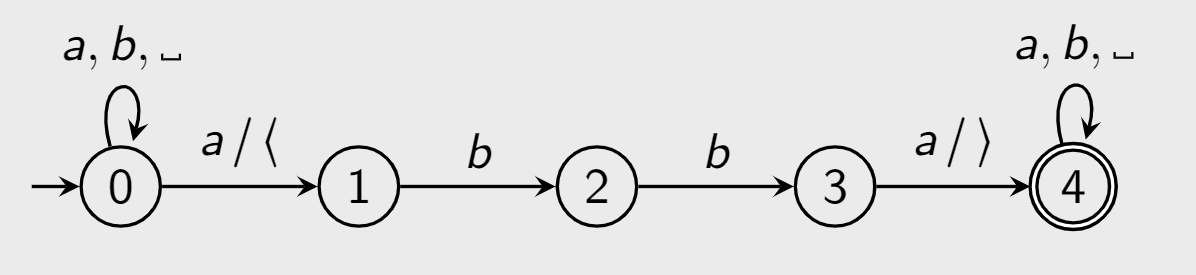
\includegraphics[scale=0.5]{img/cap6/ejemplo15_1.png}
        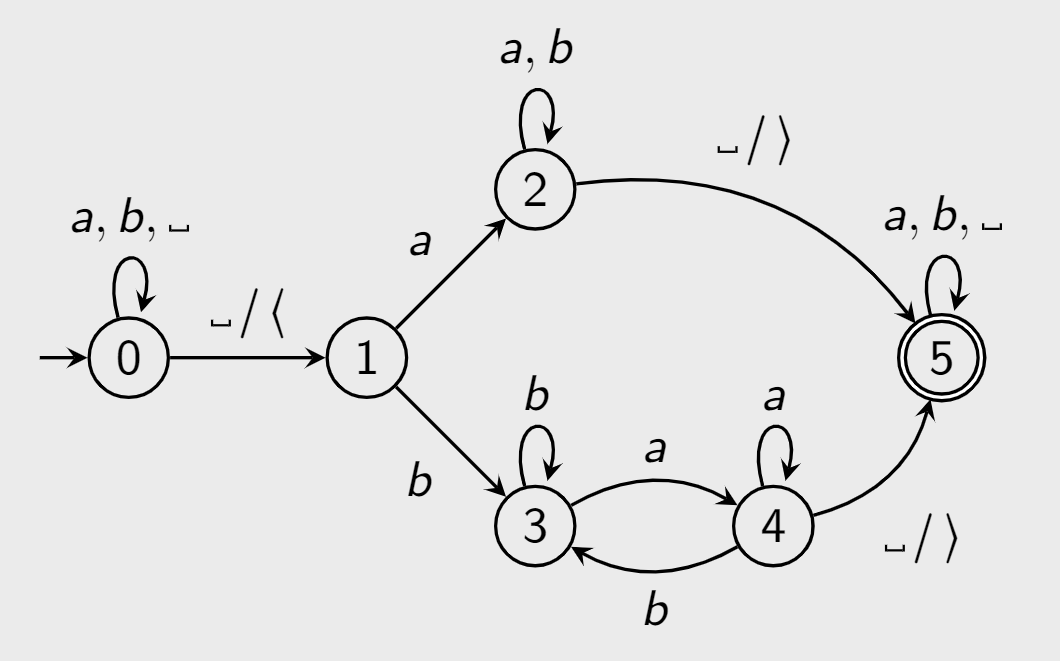
\includegraphics[scale=0.5]{img/cap6/ejemplo15_2.png}
    \end{figure}
}

\teorema{}{}{
Para todo AnnA $\ca{N} = (Q, \Sigma, \Lambda, \Delta, I, F)$, existe un AnnA I/O-determinista $\ca{N}^\text{det}$ tal que
$$
    \llbracket \mathcal{N} \rrbracket=\llbracket \mathcal{N}^{\text {det}} \rrbracket
$$
}

\paragraph{Demostración teorema 34.} Considere la determinización de $\ca{N}$ como:
$$
\mathcal{A}^{\text{det}}=\left(2^Q, \Sigma, \Lambda, \Delta^{\text{det}}, q_0^{\text{det}}, F^{\text{det}}\right)
$$
donde:
\begin{itemize}
    \item $2^Q=\{S \mid S \subseteq Q\}$ es el conjunto potencia de $Q$.
    \item $q_0^{\text{det}}=I$
    \item $\Delta^{\operatorname{det}}: 2^Q \times(\Sigma \cup \Sigma \times \Lambda) \rightarrow 2^Q$ tal que para todo $t \in \Sigma \cup(\Sigma \times \Lambda)$:
    $$
    \Delta^{\text{det}}(S, t)=\{q \in Q \mid \exists p \in S.\ (p, t, q) \in \Delta\}
    $$
    \item $F^{\text{det}}=\left\{S \in 2^Q \mid S \cap F \neq \varnothing\right\}$. \hfill $\blacksquare$
\end{itemize}











%----------------------------------------------------------------------------------------

\end{document}
